\documentclass[PhD,Submit,ngerman,UKenglish]{scrbook}
%------------------------------------------------------------------------------
% This file contains a skeleton thesis for
% a Physics or Astronomy Institute in the University of Bonn

% Specify the thesis type as an option: PhD, Master, Diplom, Bachelor
% Specify the thesis stage as an option: Draft (default), Submit, Final, PILibrary

% Specify the language(s) in the class and then use babel.
% If you need more than one language, give the default language last,
% e.g. ngerman,UKenglish for a thesis in British (UK) English where you want
% to be able to set the language to German for some part of it.

%------------------------------------------------------------------------------
% Pass TeX Live version to the package
% Use command pdflatex --version to find out which version you are running
% Add option backref=false when your thesis is ready to turn off back-referencing
% in your bibliography
\usepackage[texlive=2016,biblatex=false,newtx=false,txfonts=true]{ubonn-thesis}
% Adjustments to standard biblatex style
% \usepackage{ubonn-biblatex}

% Glossary package
\usepackage[acronym,toc,nosuper,nonumberlist]{glossaries}
% TikZ packages and libraries
% \usepackage{tikz}
% \usepackage{tikz-3dplot}
% \usepackage{pgfplots}
% \usetikzlibrary{positioning,shapes,arrows}
% \usetikzlibrary{decorations.pathmorphing}
% \usetikzlibrary{decorations.markings}
\usepackage{thesis_defs}
\usepackage{todonotes}
\usepackage{amsmath}
\usepackage{placeins}
\usepackage[numbers, sort&compress]{natbib}
\usepackage{multirow}
\usepackage{array}
\usepackage{caption}
\usepackage{subcaption}
% \usepackage{devnag}
% \usepackage[labelfont=bf]{caption}

% \usepackage{lmodern}
%------------------------------------------------------------------------------
% Instead of colouring  links, cites, table of contents etc.
% put them in a coloured box for the screen version.
% This is probably a good idea when you print your thesis.
\hypersetup{colorlinks=false,
  linkbordercolor=blue,citebordercolor=magenta,urlbordercolor=darkgreen
}

%------------------------------------------------------------------------------
% When writing your thesis it is often helpful to have the date and
% time in the output file. Comment this out for the final version.
% \ifoot[\today{} \thistime]{\today{} \thistime}

% In order to check if your labels are referenced try the refcheck package
% \usepackage{refcheck}

%------------------------------------------------------------------------------
% biblatex is included by ubonn-thesis. Look there for the settings used.
% See the options for settings that can be changed easily.
% For further changes copy the \RequirePackage[...]{biblatex} here
% and include ubonn-thesis with the option biblatex=false.

% Specify the bibliography files here and not at the end!
% Use standard_refs-bibtex if you use bibtex8
% and standard_refs-biber  if you use biber
% \addbibresource{thesis_refs.bib}
% \addbibresource{../refs/standard_refs-biber.bib}

%------------------------------------------------------------------------------
% The following definitions are used to produce the title pages
% needed at various stages
\newcommand{\thesistitle}{Enhancing Sensitivity for Ultra-High Energy Down-Going Neutrino Detection with the Pierre Auger Observatory}
\newcommand*{\thesisauthor}{Srijan Sehgal}
\newcommand*{\thesistown}{Wuppertal}
\renewcommand*{\InstituteName}{\BUWfac}
\renewcommand*{\inInstitute}{\inBUWfac}
\renewcommand*{\InstituteAddress}{\BUWaddress}
% Adjust \thesisreferee...text depending on male/female referee
\newcommand*{\thesisrefereeonetext}{1.\ Gutachter}
\newcommand*{\thesisrefereeone}{Prof.\ Dr.\ Karl-Heinz Kampert}
\newcommand*{\thesisrefereetwotext}{2.\ Gutachter}
\newcommand*{\thesisrefereetwo}{Prof.\ Dr.\ Jaime Alvarez Muñiz}
% Date when thesis was submitted (Master/Diplom)
% Year or Month, Year when thesis was submitted (PhD)
\newcommand*{\thesissubmit}{16.12.2019}
% \newcommand*{\thesissubmit}{Month 2016}
% Date of thesis examination (PhD)
\newcommand*{\thesispromotion}{16.12.2016}
% Month and year of the final printed version of the thesis
\newcommand*{\thesismonth}{December}
\newcommand*{\thesisyear}{2024}
\newcommand*{\thesisnumber}{BONN-IR-2019-XXX}
% Command to horizontal cenetr the table contents
\newcolumntype{P}[1]{>{\centering\arraybackslash}m{#1}}
\captionsetup[figure]{labelfont=bf,format=hang}
\captionsetup[table]{labelfont=bf,format=hang}
% Command for Offline symbol 
\newcommand{\Offline}{\mbox{$\overline{\textrm{Off}}$\hspace{.05em}%
    \raisebox{.4ex}{$\underline{\textrm{line}}$}}}
%------------------------------------------------------------------------------
% The abstract is only needed for the printed version and should be in
% English regardless of the language of the thesis
\newcommand{\thesisabstract}{%
  \begin{otherlanguage}{UKenglish}
    This is your thesis abstract. It may be in a language that is
    different from the rest of your thesis.
  \end{otherlanguage}
}

%------------------------------------------------------------------------------
% \includeonly can be used to select which chapters you want to process
% A simple \include command just inserts a \clearpage before and after the file
% Note that \includeonly can be quite picky! Do not forget to put a
% comma after the filename, otherwise it will simply be ignored!
% \includeonly{%
%   thesis_intro,
%   thesis_appendix,
%   thesis_acknowledge
% }

%------------------------------------------------------------------------------
% Give a list of directories where figures can be found. Do not leave
% any spaces in the list and end the directory name with a /
\graphicspath{%
  {../figs/}%
  {../figs/cover/}%
  {../figs/graphics/}%
  {../feynmf/}%
}

%------------------------------------------------------------------------------
% Make a glossary and a list of acronyms
% \makeglossaries
\makenoidxglossaries

% Glossary entries
%
% Contains a list of glossary definitions to illustrate how a glossary
% using the glossaries package
%

\newglossaryentry{siunitx}{name=siunitx,
  description={the best package around for typesetting units}}
\newglossaryentry{csquotes}{name=csquotes,
  description={a very nice package for using consistent quotes that is
  language sensitive}}
\newglossaryentry{LaTeX}{name=\LaTeX,
  description={the typesetting program that is used for this guide}}


\newacronym[plural=CRs,firstplural=cosmic rays (CRs)]{CR}{CR}{cosmic ray}  
\newacronym[plural=UHECRs,firstplural=ultra-high energy cosmic rays (UHECRs)]{UHECR}{UHECR}{ultra-high energy cosmic ray}  
\newacronym{UHE}{UHE}{ultra high energy}
\newacronym{UHEnu}{UHE$\nu$}{Ultra high energy neutrino}
\newacronym{UHEnus}{UHE$\nu$}{ultra high energy neutrinos}
\newacronym{SD}{SD}{Surface Detector}
\newacronym{FD}{FD}{Fluorescence Detector}
\newacronym{HEAT}{HEAT}{High Elevation Auger Telescope}
\newacronym[first= \textit{lateral distribution function} (LDF)]{LDF}{LDF}{lateral distribution function}
\newacronym{EM}{EM}{electromagnetic}
\newacronym{MVA}{MVA}{multivariate analysis}
\newacronym{AUGER}{AUGER}{Pierre Auger Observatory}
\newacronym[plural=EASs,firstplural= Extensive Air Showers (EASs)]{EAS}{EAS}{extensive air shower}
\newacronym{VEM}{VEM}{vertical equivalent muon}
\newacronym{MoPS}{MoPS}{Multiplicity-of-Positive-Steps}
\newacronym{FADC}{FADC}{flash analog-to-digital converter}
\newacronym{GZK}{GZK}{Greisen–Zatsepin–Kuzmi}
\newacronym{ToT}{ToT}{time-over-threshold}
\newacronym{ToTd}{ToTd}{Time-over-Threshold-deconvolved}
\newacronym{DGL}{DG$\mathrm{_{low}}$}{down-going low}
\newacronym{DGH}{DG$\mathrm{_{high}}$}{down-going high}
\newacronym{ES}{ES}{Earth-skimming}
\newacronym{TA}{TA}{Telescope Array}
\newacronym{CNB}{CNB}{Cosmic Neutrino Background}
\newacronym{CMB}{CMB}{Cosmic Microwave Background}
\newacronym{ISM}{ISM}{interstellar medium}
\newacronym{AGN}{AGN}{Active Galactic Nuclei}
\newacronym{eV}{eV}{electronvolts}
\newacronym{HESS}{HESS}{High Energy Stereoscopic System}
\newacronym{CTA}{CTA}{Cherenkov Telescope Array}
\newacronym{EBL}{EBL}{extragalactic background light}
\newacronym{WIMP}{WIMP}{Weakly Interacting Massive Particle} 
\newacronym{CC}{CC}{Charged Current}
\newacronym{NC}{NC}{Neutral Current}
\newacronym{QCD}{QCD}{quantum chromodynamics}
\newacronym{MHz}{MHz}{megahertz}
\newacronym{GHz}{GHz}{gigahertz}
\newacronym{UV}{UV}{ultraviolet}
\newacronym{IACT}{IACT}{Imaging Cherenkov telescope}
\newacronym{PMT}{PMT}{photomultiplier tube}
\newacronym{RD}{RD}{Radio Detector}
\newacronym{UMD}{UMD}{Underground Muon Detector}
\newacronym{CLF}{CLF}{Central Laser Facility}
\newacronym{XLF}{XLF}{eXtreme Laser Facility}
\newacronym{WCD}{WCD}{Water Cherenkov Detector}
\newacronym{VCT}{VCT}{vertically central through-going}
\newacronym{TH}{TH}{threshold trigger}
\newacronym{UUB}{UUB}{upgraded unified board}
\newacronym{ADST}{ADST}{Advanced Data Summary Tree}
\newacronym{AoP}{AoP}{Area over Peak}
\newacronym{MC}{MC}{Monte Carlo}
\newacronym{GDAS}{GDAS}{Global Data Assimilation System}
\newacronym{FDA}{FDA}{Fisher Discriminant Analysis}
\newacronym{LDA}{LDA}{Linear Discriminant Analysis}
\newacronym{FOV}{FOV}{field of view}





% Draft version - add DRAFT to header.
% You can use draftwatermark to add DRAFT to the cover page.
% Note that this only works if \unitlength is set to 1pt.
% This is normally not the case - it is set to 1mm in ubonn-thesis.sty.
% The background package is used for later versions of TeX Live.
%\setlength{\unitlength}{1pt}
% \ifthenelse{\equal{\ThesisVersion}{Draft}}{%
%   \usepackage{background}
%   \ifthenelse{\texlive < 2013}{%
%     \SetBgContents{DRAFT}
%     \SetBgColor{blue!30}
%   }{%
%     \backgroundsetup{contents=DRAFT, color=blue!30}
%   }
% }

%------------------------------------------------------------------------------
\begin{document}

% Cover page of thesis - this is only needed for the printed final
% version to be submitted to the department library
% Do not use this page for thesis submission to the Prüfungsamt or Promotionsbüro!
\ifthenelse{\equal{\ThesisVersion}{PILibrary}}{%
  \typeout{Document \jobname, Info: PI library version of thesis}
  \input{../cover/\ThesisType_Cover}
}{}

% Start counting pages from the title page
\frontmatter
% Dedication has to come before \maketitle
% \dedication{For ...}

% Select the correct title page(s)
\ifthenelse{\equal{\ThesisType}{Unknown}}{%
  \typeout{Document \jobname, Error: Unknown thesis type - no title page printed}
}{%
  % Bachelor thesis only has one title page
  \ifthenelse{\equal{\ThesisType}{Bachelor}}{%
    \typeout{Document \jobname, Info: Bachelor thesis}
    \input{../cover/\ThesisType_Title}
  }{%
    \ifthenelse{\equal{\ThesisVersion}{Final} \OR \equal{\ThesisVersion}{PILibrary}}{%
      % Final and PI library versions
      \typeout{Document \jobname, Info: Final version of a \ThesisType  thesis}
      \input{../cover/\ThesisType_Final_Title}
    }{% Submission and draft versions
      \input{../cover/\ThesisType_Submit_Title}
      \typeout{Document \jobname, Info: Draft/submission version of a \ThesisType  thesis}
    }
  }
}

\pagestyle{scrplain}

%------------------------------------------------------------------------------
% You can add your acknowledgements here - don't forget to also add
% them to \includeonly above
%------------------------------------------------------------------------------
\chapter*{Acknowledgements}
\label{sec:ack}
%------------------------------------------------------------------------------
Even though this thesis has my name on the front a number of people were involved in shaping its final form both in person and in spirit.

First and foremost I would like to thank my late grandfather Shanti Sarup Sehgal and grandmother Kusum Sehgal. Their constant motivation and belief in my abilities has and will always inspire me to achieve more.

I am very grateful to Professor Bernhard Ketzer for giving me an opportunity to write my thesis in his group. In spite of my many shortcomings and failures he has always been patient and supportive during the entire time and has been a role model I look up to. I would also like to thank Professor Jochen Dingfelder. I have always admired your lectures and am thankful that you agreed to be my second supervisor.

A special thanks to PhD students Michael Hösgen and Martin Hoffmann for helping with the editing of this thesis. Thank you to Michael for always answering my various questions and solving my problems without which this thesis would have never been completed. A big thanks to the whole AG Ketzer group for both the academic and moral support.

I am grateful to my father Ravi Sehgal, my mother Rajni Sehgal and my brother Sambhav for all the sacrifices they have made. Without their constant support studying at Bonn would have just remained a pipe dream. Lastly, I am thankful to the wonderful set of friends I am lucky to have. Thank you Svenja ,Georgios and Amitayus for the countless Mensa lunches which helped me remain sane throughout the thesis.

%%% Local Variables:
%%% mode: latex
%%% TeX-master: "../mythesis"
%%% End:


\tableofcontents

\mainmatter
\pagestyle{scrheadings}

% Turn off DRAFT for the following pages
%\ifthenelse{\equal{\ThesisVersion}{Draft}}{%
%  \ifthenelse{\texlive < 2013}{%
%    \SetBgContents{}
%  }{%
%    \backgroundsetup{contents={}}
%  }
%}{}

%------------------------------------------------------------------------------
% Add your chapters here - don't forget to also add them to \includeonly above
% !TEX root = mythesis.tex

%==============================================================================
\chapter{Introduction}
\label{sec:intro}
%==============================================================================
\begin{figure}[h!]
\centering
  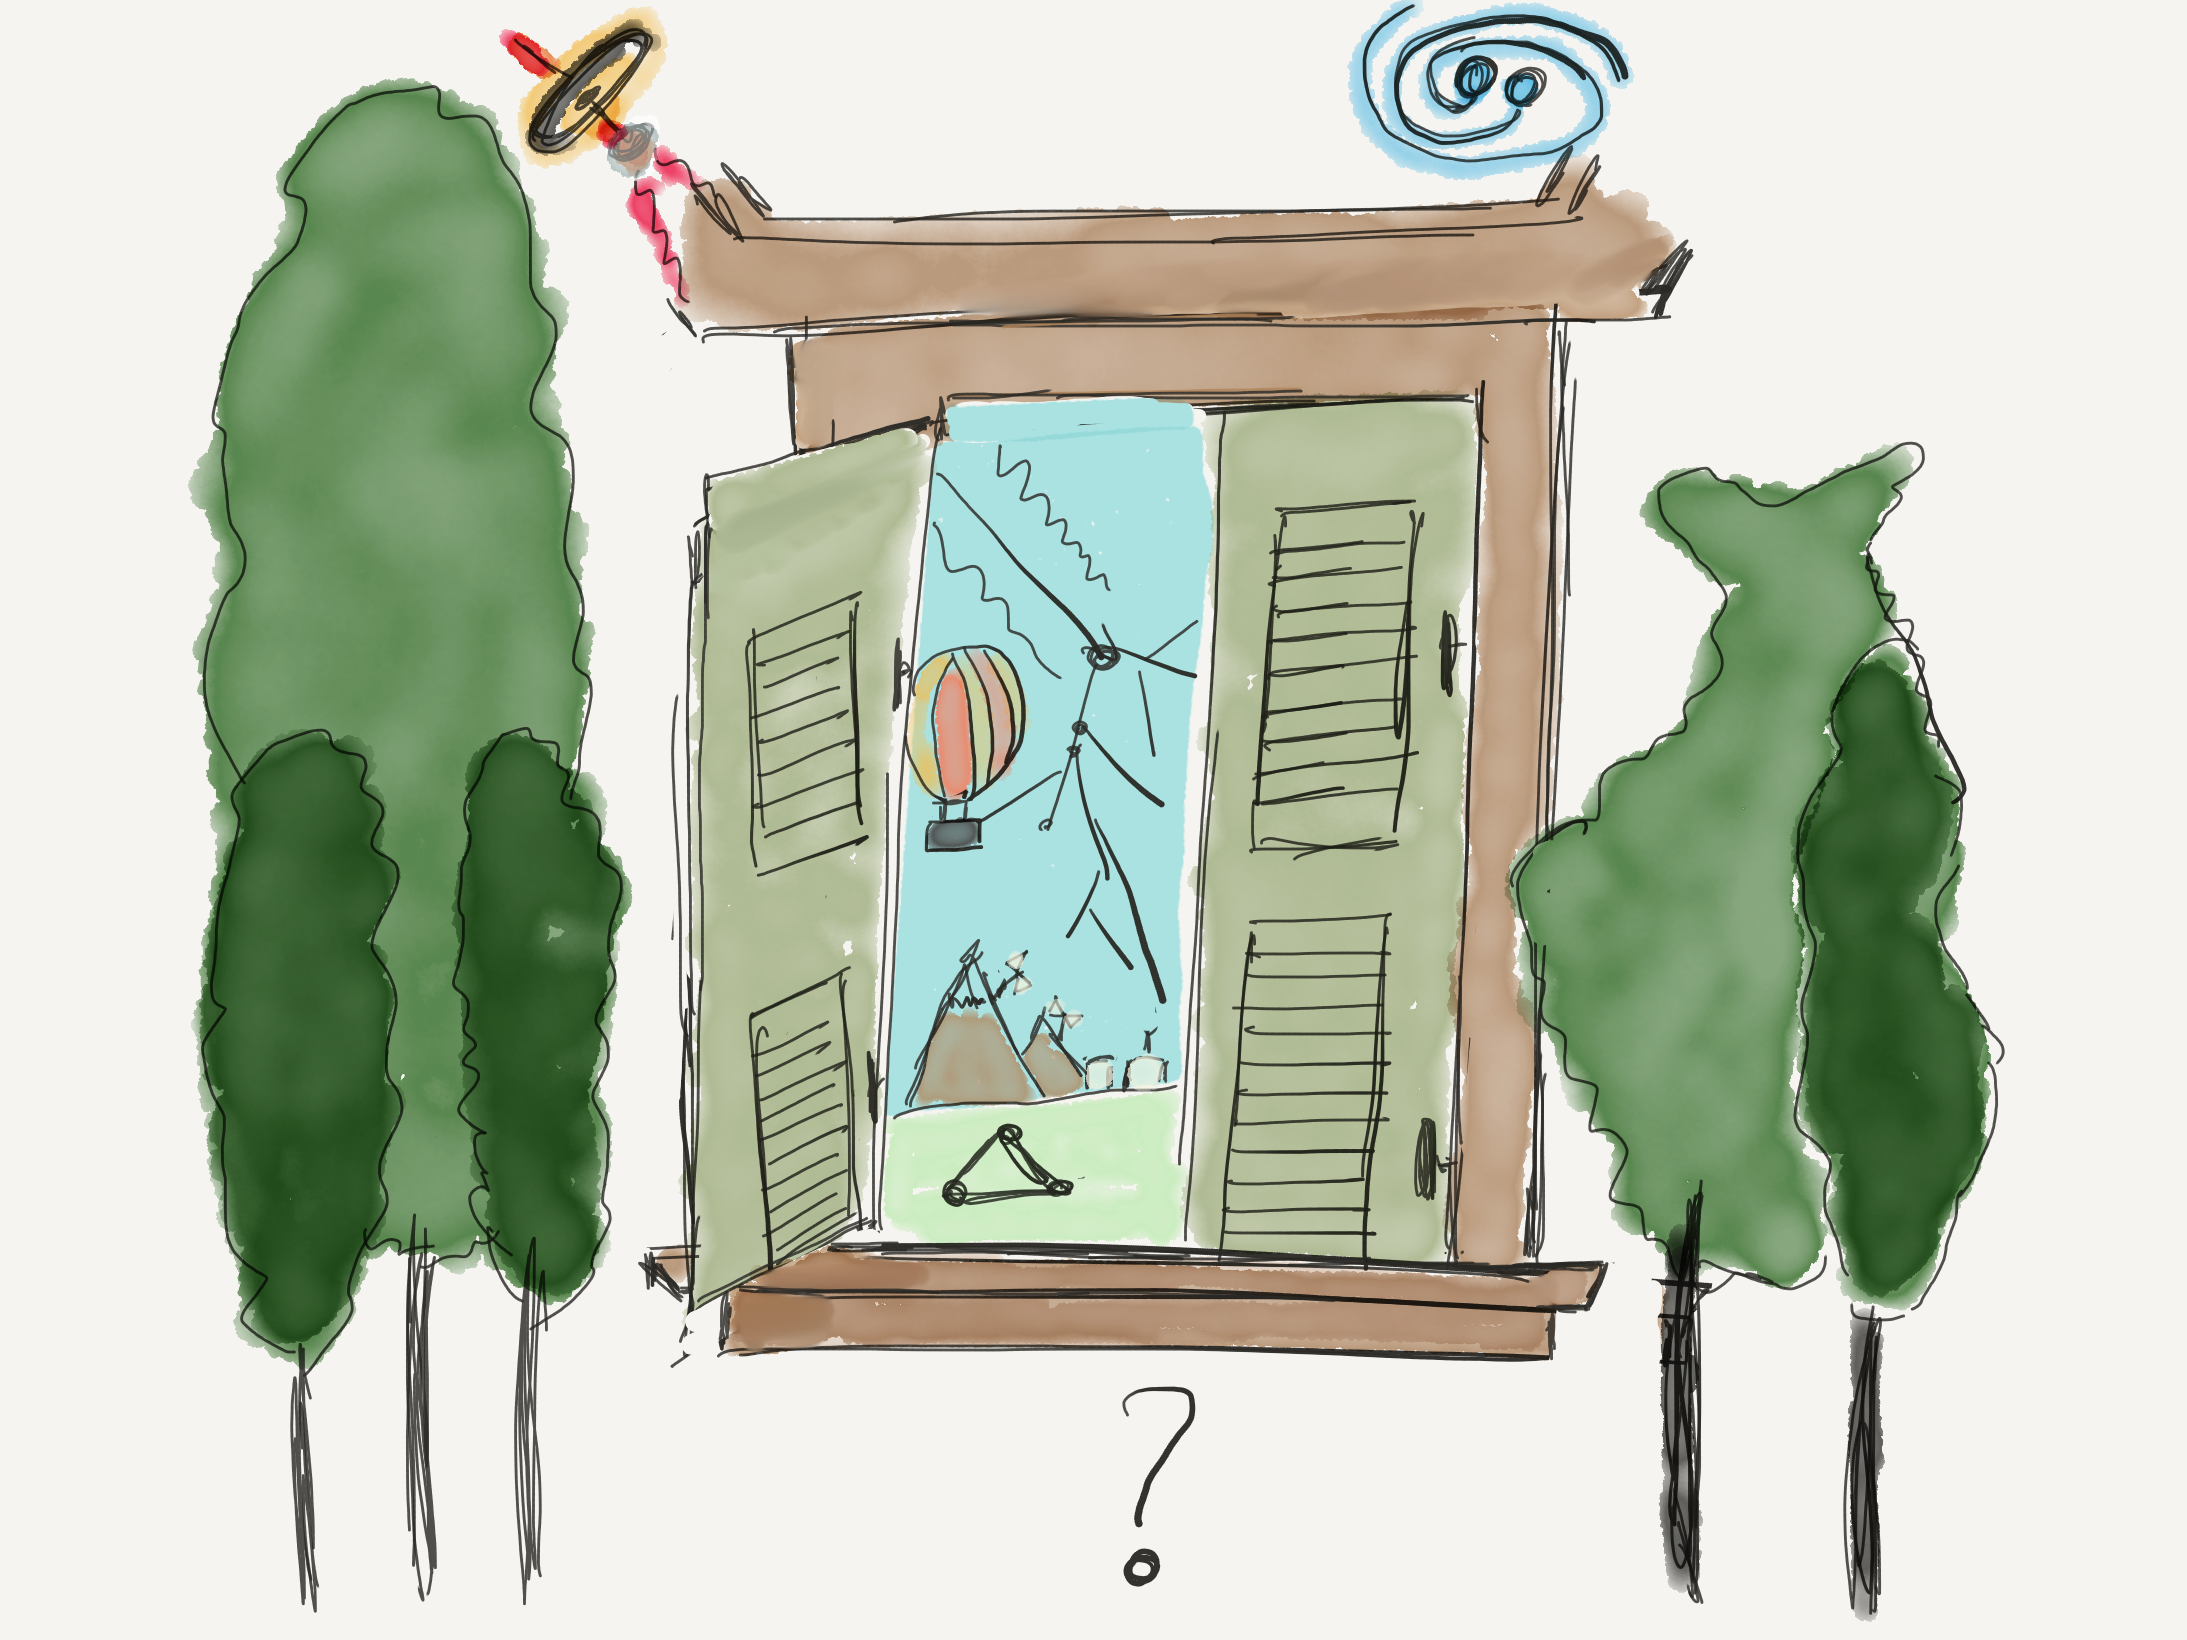
\includegraphics[width=13cm]{thesis_figures/What?.png}
\caption{Window to the inner workings of the Universe is only half opened. (better caption?)}
\label{fig:intro}
\end{figure}
The need to understand how something works or why something is? is ingrained in every human. While attempting to find answers for these questions one either answers them conclusively or finds oneself asking additional questions stemming from the original. One such question which bothered physicists at the beginning of the 20th century and eventually led to the field of \textit{astro-particle physics} was of so-called "atmosphere electricity" or ionization of air. After the pioneering discoveries by Theodor Wulf~\cite{article_Wulf} and Victor Hess~\cite{Hess:1912srp} who found the increase of this ionization rate with altitude and theorized the origin of this radiation to be not earth but something above our atmosphere, the name \textit{cosmic rays} was coined by Robert Millikan who believed these rays were originating from primary photons. This hypothesis was rejected by the measurements done by Jacob Clay~\cite{Clay:1927I,Clay:1928II} in 1927 who observed a latitude dependence of the intensity of cosmic rays concluding this to be a deflection of the primary cosmic-rays(CRs) by the geomagnetic field of the earth which indicated that these rays must be charged particles. After this came the efforts of B. Rossi~\cite{rossi1933eigenschaften}, German group~\cite{schmeiser1938harten} and P. Auger~\cite{RevModPhys.11.288} all independently discovering coincident signals in separated Geiger counters which they explained by the counters being struck by an extensive particle shower triggered by a primary cosmic ray. The phenomenon was named \textit{sciami} by Rossi, \textit{Luftshauer} by the German group and "Auger showers" by Auger and his collaborators. Auger went one step further by further estimating the primary energy of the cosmic ray via his superior setup giving rise to some questions about CRs which are yet unanswered, how are they created and where are they coming from. One of the known sources which is the Sun is too close to explain some other high energy CRs constantly hitting the Earth's atmosphere. Since then the field has only expanded with numerous experiments set up to characterize these cosmic rays. 

The biggest of these experiments which looks for ultra-high energy cosmic rays(UHECRs) exists in 3000 km$^2$ patch of Argentinian pampa just outside Malargue called the Pierre Auger Observatory~\cite{Auger:2015}. It uses a combination of 1660 Water Cherenkov tanks which form the Surface Detector of the observatory and observe the air shower particles arriving at the ground along with Fluorescence Detectors/Telescopes which can look at the development of shower as it travels through the atmosphere. Built primarily to answer the question of the cut-off of the cosmic ray spectrum also known as Greisen–Zatsepin–Kuzmin limit(or GZK cut-off), the observatory has provided immense contributions not only in the field of CRs but also in the fields of Geophysics(elves)~\cite{Mussa_2022}, Dark matter(composition)~\cite{Abreu_2023} and multi-messenger physics(neutrino+photon searches)~\cite{Aab_2019_point,Auger_photons_2022}. Currently, the Surface detector is undergoing an upgrade which will add a scintillator and radio detector on top of the Water Cherenkov tanks further increasing the sensitivity of the Observatory especially to the composition of the cosmic rays.

The non-electrical neutrality of the incoming CRs provides one of the biggest hindrance for finding their sources. This means that CRs do not travel in straight lines from their sources and are affected by the magnetic fields and can also interact with the matter along the way~\cite{bister2024largescaleanisotropyfluxdemagnification, ALLARD201233}. Combined with the fact that the possible sources are light years away from us, without knowing the magnetic fields of the Universe it is very hard to detect the sources of CRs. Ultra High Energy Neutrinos (UHE$\nu_s$) can help in this challenging search for the sources of CRs~\cite{UHEcorrelation_2016}. Being electrically neutral and having a very low interaction cross-section these particles can travel large distances unaffected by the intervening matter and magnetic fields. Several scenarios which are discussed later in section.~\ref{subsubsec:CRmessengers} describe how the UHE$\nu_s$ can be produced by cosmic-rays and can tell us about their sources. Moreover, UHE$\nu_s$ are also interesting as they can also help constrain or explain different production and propagation scenarios for various sources helping us see known astrophysical and cosmogenic objects in a new way. The success of IceCube Neutrino Observatory, a neutrino observatory located in the South Pole,  in detecting the first astrophysical neutrinos and observations of the first steady source NGC 1068~\cite{Icecube_2022} and transient source~\cite{Icecube_txs} have reinvigorated the astro-particle field. The Pierre Auger Observatory has also contributed to the search for UHE$\nu_s$ by trying to detect the Extensive Air SHowers (EASs) that can be induced by them. With its stellar sensitivity at high energy, searches at Pierre Auger Observatory have provided some of the strictest upper limits on the diffuse flux of UHE neutrinos~\cite{Aab_2019_diffuse}. This has already led to constrains on various hypothesized models explaining cosmogenic neutrino production.

The last decade with the successes of LIGO/VIRGO~\cite{PhysRevLett.116.061102} in measuring the first Gravitational waves and IceCube in detecting the first astrophysical neutrinos has also rekindled a field which displays the true spirit of harmony in science and is called multi-messenger astronomy. The aim of the field is to establish a network that can coalesce all the information available through various messengers via which we can see the Universe and maximise the resources and experiments available at Earth. This also allows us to understand the sources better since the observation or non-observation of different messengers can help constrain the mechanisms behind their functioning. The beginning of this field can be traced back to the observation of the first cosmic rays in conjunction with solar flares further cementing the important role Pierre Auger Observatory can play for this field. One of the most important success stories of this field is the August 2017 detection of the neutron star collision~\cite{Abbott_2017} first by the LIGO/VIRGO detector since the Gravitational waves are the fastest messengers and then 1.7s later by the Fermi Gamma ray space telescope and INTEGRAL. 11 hours later already alerted by these two experiments the optical counterpart was detected by multiple telescopes like Las Campanas Observatory and the Hubble Space Telescope. The event was also further seen in Ultraviolet(Neil Gehrels Swift Observatory), X-ray(Chandra X-ray Observatory) and radio(Karl G. Jansky Very Large Array). The non observation of neutrinos by both the IceCube and the Pierre Auger Observatory helped reach the important conclusion about the orientation of the jets which is hypothesized to be off-axis i.e. not pointing directly towards the Earth. Since neutrinos and Gravitational waves are the fastest of the messengers to reach the Earth, alerts issued by IceCube and LIGO/VIRGO are regularly used to follow up the events with other experiments. Subsequent observations of the blazar TXS 0506+056~\cite{TXS_Multi_2018} with IceCube, FERMI-LAT and MAGIC and the observations of neutrinos from the plane of the Milky Way galaxy~\cite{Galactic_plane_nu_2023} have helped establish the continued importance of multi-messenger astronomy.

In this thesis performance of one of the upgrades of the Pierre Auger Observatory done in 2013 is evaluated in the context of neutrino search. This upgrade consisted of introducing new triggers called Time over Threshold deconvulated(ToTd) and Multiple of Positive Steps(MoPS) to reduce the muonic background and effectively decrease the energy threshold for the array. Such triggers can be particularly important in the context of neutrino searches between $60^\circ$-$75^\circ$ since they help in getting a better signal background separation. The effect of these triggers for both the search of a diffused neutrino flux and point like sources of neutrinos is investigated. The thesis also focuses on maximising the previously done neutrino searches in the zenith region $60^\circ$-$75^\circ$ by investigating and updating the analysis presented in~\cite{Aab_2019_diffuse},~\cite{gap_note_2013}.

The thesis is structured as follows, The next chapter~\ref{chap:crnNu} gives the theoretical background for UHE cosmic rays and UHE neutrinos and other important messengers in regard to the Pierre Auger Observatory. It also aims to discuss the various theoretical scenarios involved in their production and propagation. The chapter also aims to summarize the important recent results for these messengers and the various interesting open questions for them. The next chapter~\ref{chap:EAS} describes the phenomenon of Extensive Air showers which is used to indirectly detect both the cosmic rays and neutrinos at the Pierre Auger Observatory. To continue with understanding the detection in a more experimental context the next chapter~\ref{chap:setup} gives a detailed description of the Pierre Auger Observatory. The objective of the chapter is to try to give an exhaustive description of all the tools at the Pierre Auger Observatory necessary to detect neutrinos with a particular focus on the Surface Detector which is of primary concern for the analysis presented in this thesis. A small section is also dedicated to the recently completed AugerPrime upgrade and the exciting potential it offers especially for multi-messenger searches. 

The second part of the thesis is dedicated to the neutrino search in the zenith angular region $60^\circ$-$75^\circ$ (Down-going low, DG$\mathrm{_{low}}$). This part begins with the chapter~\ref{chap:DGL} that gives a description of the neutrino search in the angular range $60^\circ$-$75^\circ$ which is also the primary focus region for this thesis. The chapter is dedicated to provide a complete description of the choices made for the analysis with the proper reasoning. It reports the areas of potential improvements and also communicates the observed improvements to the neutrino search with the new triggers. A new ~\textit{blind} search is performed to look for neutrinos in the data recorded at the Pierre Auger Observatory. The results are summarised at the end of this chapter and due to the non-observance of any neutrino like events, the corresponding limits to the neutrino flux are presented. The Observatory can also detect showers in zenith angle range $75^\circ$-$90^\circ$ (Down-going high, DG$\mathrm{_{high}}$) and up-going showers in the zenith angular region $90^\circ$-$95^\circ$ (Earth-skimming, ES)with the Surface Detector and $90^\circ$-$180^\circ$ (???) with the Fluorescence Detector, but these searches are not performed in this thesis and only their final results are included for comparison and to provide a holistic feel for the neutrino search at Pierre Auger Observatory.

The last part of this thesis presents an example of a neutrino follow-up analysis for point-like sources in chapter~\ref{chap:follow-up}. Due to the non-observance of any neutrinos in the data at the Pierre Auger Observatory an upper limit set by this analysis is also provided for interesting point source neutrino candidates. All the important results are then finally summarised in chapter~\ref{chap:conc} and a short outlook of the future directions for the analysis and the neutrino search at the Pierre Auger Observatory is put forward. The dissertation is completed by three appendices. The first describing the independent work done to compare the various hadronic interaction models for neutrino simulations and the second contains a technical overview of the changes made to implement the $75^\circ$-$90^\circ$ neutrino search within Offline, the software framework of the Pierre Auger Observatory. 

%%% Local Variables:
%%% mode: latex
%%% TeX-master: "mythesis"
%%% End:

% !TEX root = mythesis.tex

%==============================================================================
\chapter{Ultra High Energy Cosmic Rays and Neutrinos}
\label{chap:crnNu}
%==============================================================================

\section{Ultra High Energy Cosmic Rays}
\label{sec:UHECR}
\subsection{History}
\label{subsec:crhist}
\glspl{CR} have been a source of investigation for more than a century now. Even before the balloon flight by Victor Hess, it was Henry Becquerel, the discoverer of radioactivity, who believed that the \textit{atmospheric electricity} (ionization of air) was due to the radioactive substances present on Earth. In such a scenario the ionization rate should decrease the higher up you go in the atmosphere. The first measurements disproving this theory were performed by Theodor Wulf in 1909 with his own developed electrometer. His measurements published in the \textit{Physikalische Zeitschrift} indicated a higher level of radiation at the top of the Eiffel Tower as compared to its base. Unfortunately, the measurements were not widely accepted, and it would take three years till Victor Hess, via his several balloon flights, provided irrefutable measurements corroborating Wulf's observations.

Between 1911 and 1912 Victor Hess performed nine (2 in 1911 and 7 in 1912) balloon flights going as high as 5350 m a.s.l to measure the dependence of ionization rate to altitude. He carried with him three Wulf electrometers, two tuned for $\gamma$ rays and the third tuned for $\beta$ rays which along with $\alpha$ rays were the only three known radioactive decays. His measurements published in the Proceedings of the Viennese Academy of Sciences~\cite{Hess:1912srp},~\cite{hess2018observationspenetratingradiationseven} showed that the radiation level decreased slightly up to a certain altitude ($\sim$1 km) but after this height, the radiation increased significantly and at the highest flown altitudes reached levels about twice in comparison to the ones at sea level. Some of his measurements were done during the night and one during a partial solar eclipse which further made him rule out the Sun as a source of this radiation. With further confirmations via the measurements by Werner Kolhörster in 1914 and Robert Millikan, in 1925, Victor Hess was awarded the Nobel Prize in Physics in 1936. 

\glspl{CR} were still presumed to be gamma rays. This supposition was quickly negated by the efforts of Jacob Clay, who via his measurements of the \gls{CR} intensity at different latitudes while sailing from Java to the Netherlands in 1927~\cite{Clay:1927I}, showed that the geomagnetic field had a significant effect on the intensity. Further observations of the \textit{East-West} effect, the directional dependent intensity due to the charge of the primary \glspl{CR} as predicted by Bruno Rossi~\cite{PhysRev.36.606} by various experiments~\cite{PhysRev.43.834}~\cite{PhysRev.43.835} concluded that the intensity was greater from the west, proving that \gls{CR} primaries have a positive charge.

Today we use the term \glspl{CR} to describe the highly energetic charged particles travelling at very high speeds through space. The Earth is constantly bombarded by \glspl{CR}, some originating from the Sun but most of them from outside our Solar System. In more than 100 years since Victor Hess's balloon flights, we have gathered a lot more information and have achieved a better understanding of \glspl{CR}. We have detected \glspl{CR} up to energies $\sim 10^{20}$\gls{eV}~\cite{TA_2023} which is an impressive feat since at these energies the expected flux drops below one particle per $\text{km}^2$ yr. We know a lot more about the composition of the \glspl{CR} and have also proposed models explaining their origin and their journey to Earth. \glspl{CR} continue to be a source of fascination. Some of the achievements are summarized below along with some unanswered questions about \glspl{CR}. 

\subsection{Origin}
\label{subsec:crorig}
To understand the sources of \glspl{CR} one needs to understand the mechanisms that could impart huge amounts of energies to the tiny particles that actually reach the Earth. We already know that the low energy \glspl{CR} which reach our Earth are predominantly coming from the Sun. The evidence for this comes from the observation of an increase in these with a coincidence to the violent activity of the sun. Most of the \glspl{CR} and \glspl{UHECR}, E > $10^{18}$eV, do not exhibit this temporal coincidence and are thought to have originated in our Galaxy or beyond respectively. Two different mechanisms could explain how the CR particles obtain such high energies and travel over large distances: \textit{bottom-up}~\cite{1984ARA&A..22..425H,Blandford_2000,1993A&A...272..161R} and \textit{top-down}~\cite{Bhattacharjee_2000,Busca_2006}. The \textit{top-down} approach assumes that the \glspl{UHECR} are produced due to the decay or annihilation of extremely massive or exotic particles.
Both of these mechanisms have been investigated with various experiments including the Pierre Auger Observatory~\ref{chap:setup}. With the current observations, the top-down models face significant challenges. The extremely high energies required for the annihilation of the hypothesized exotic particles and the lack of evidence for their existence make it very difficult to both verify and rule out the top-down mechanism. The continued improvement in understanding of astroparticle physics and the early universe makes the study of \glspl{UHECR} an exciting and active area for research with the mystery of their origin and propagation still waiting for a solution. 

\begin{figure}[t!]
  \centering
  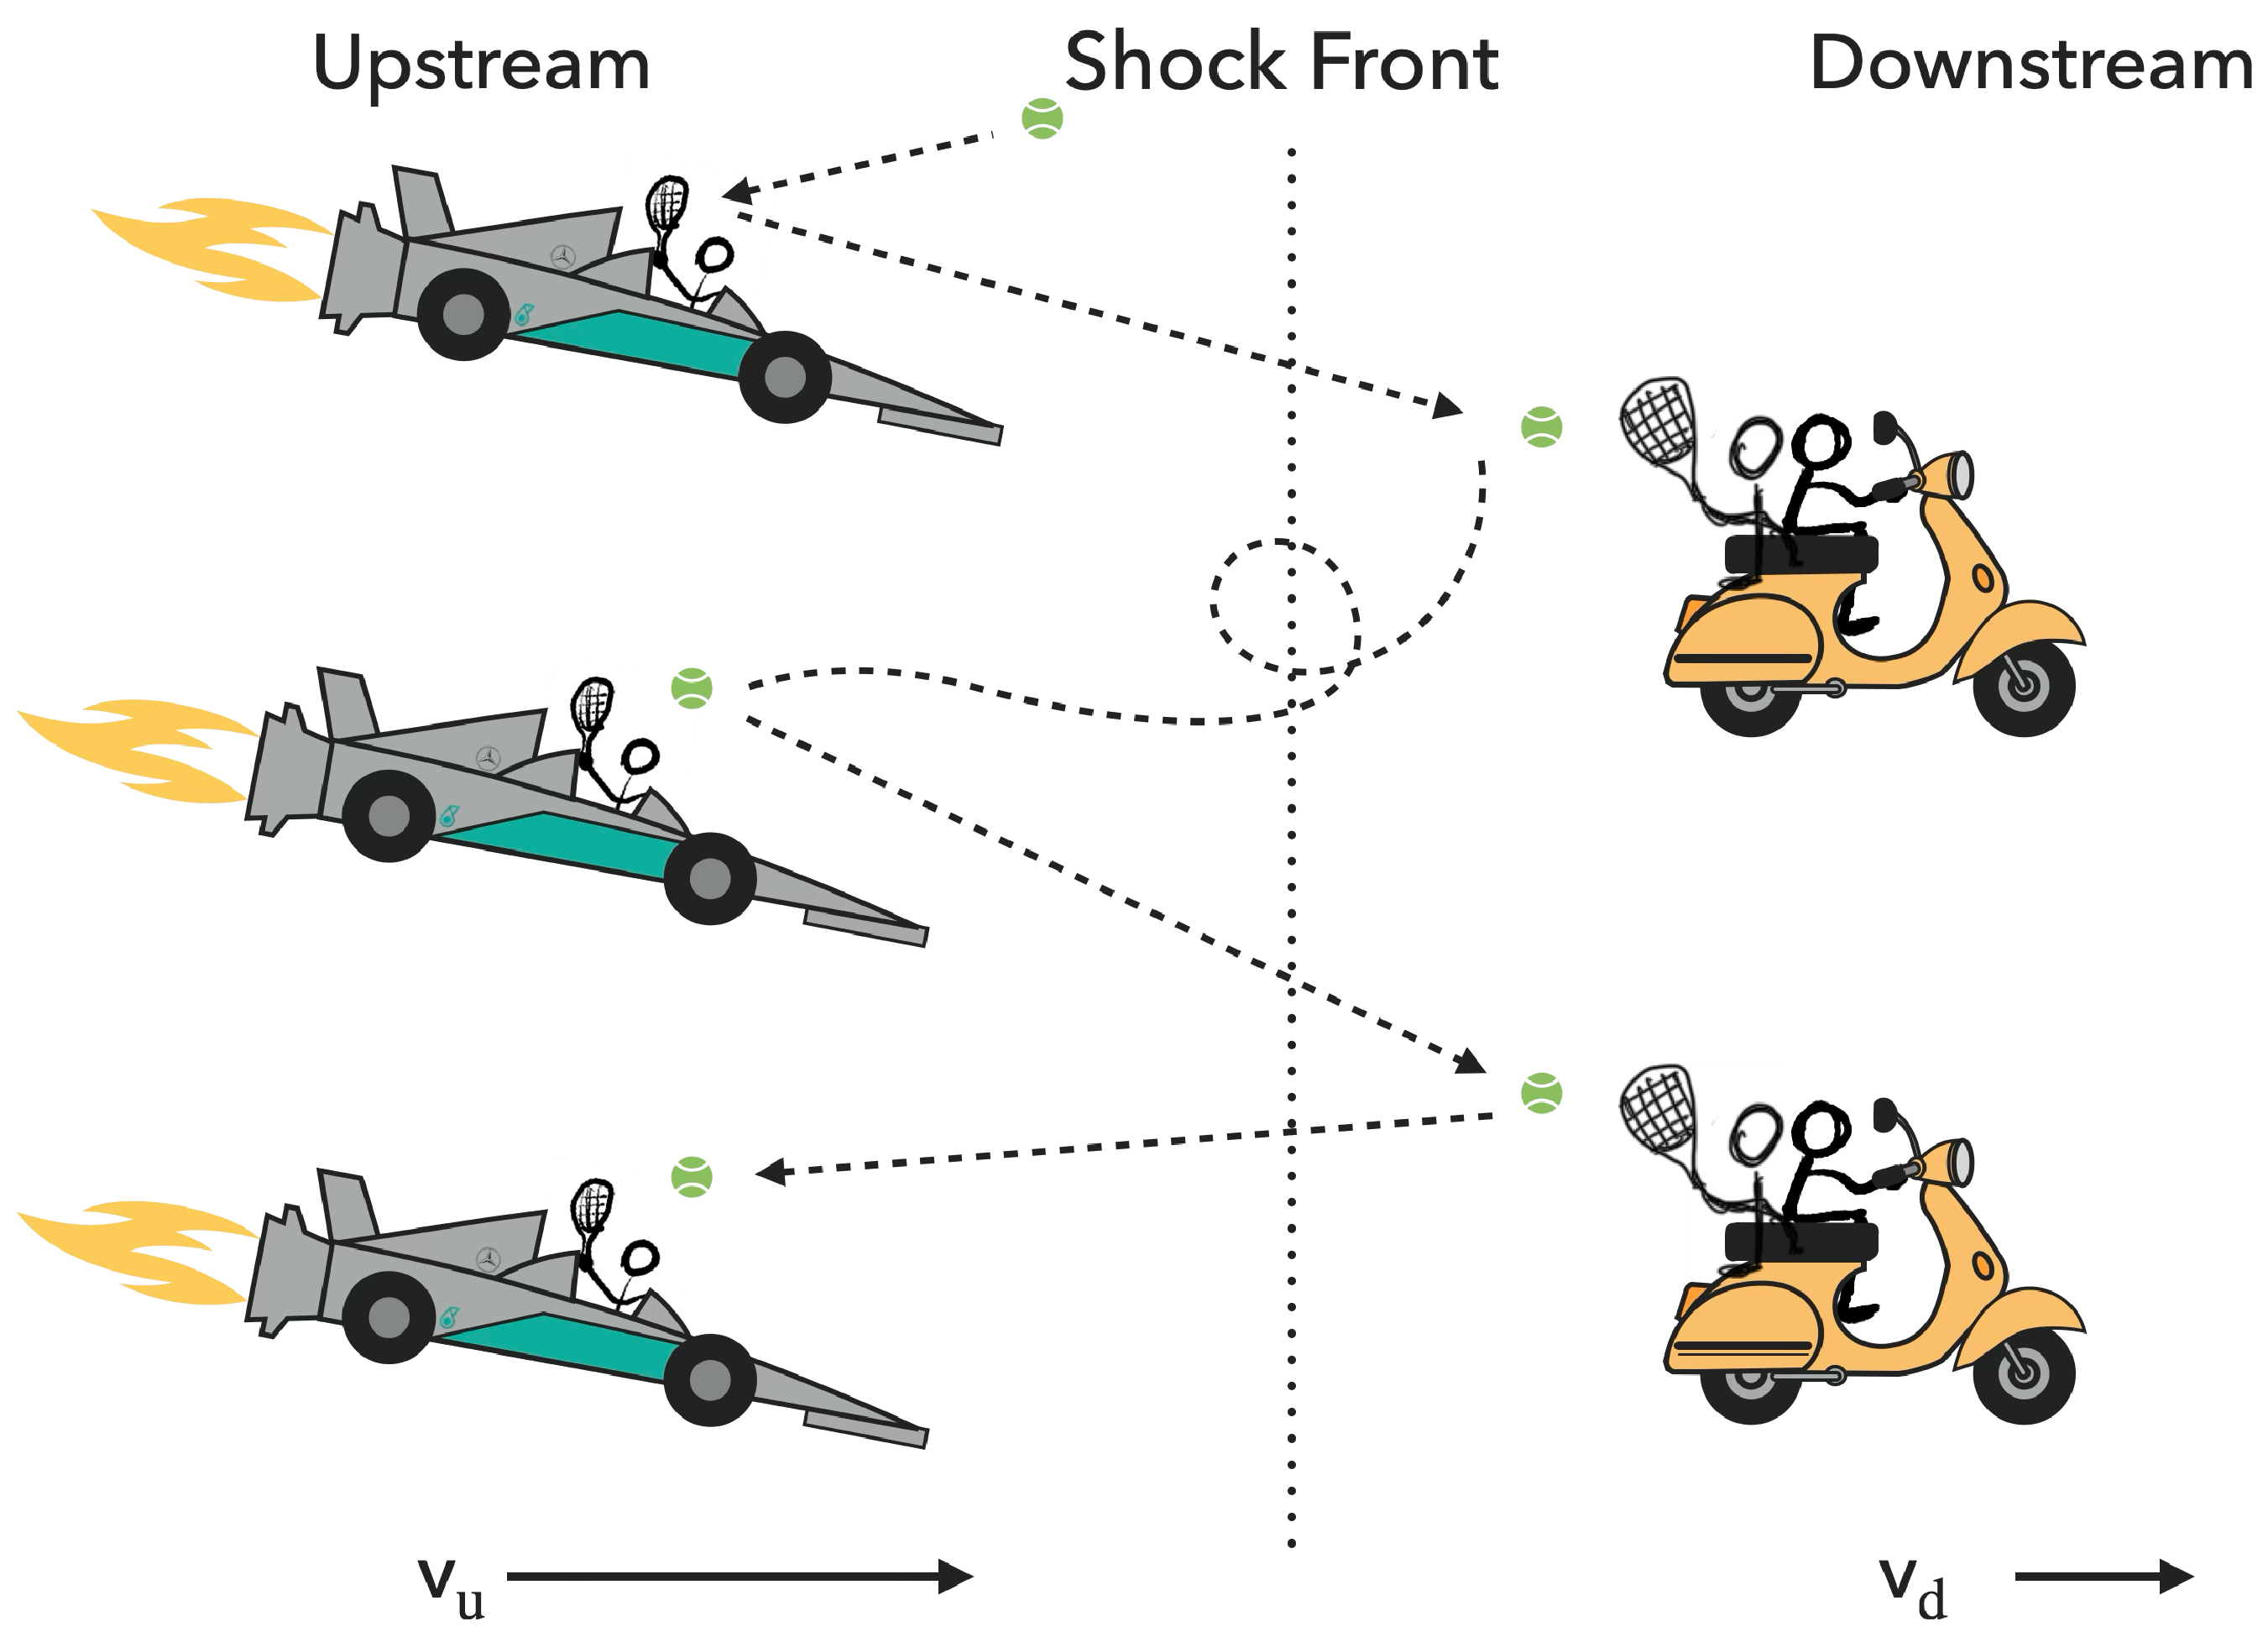
\includegraphics[width=10.5cm]{thesis_figures/CRnNu/Diffusive-shock-cartoon.pdf}
  \caption{An illustration to depict the diffusive shock acceleration mechanism and the possible trajectory in the plasma like shock front region. Figure inspired from work by M. Scholer.}
  \label{fig:Shock_cartoon}
\end{figure}

\subsubsection{Bottom-up scenario}
\label{subsec:Bupsce}
There are many proposed ways in which \glspl{CR} could get accelerated by astrophysical sources. One of the most widely accepted descriptions that can explain most of the observed \glspl{CR} that originate from our Galaxy is the diffusive shock acceleration also known as Fermi acceleration~\cite{PhysRev.75.1169}. Qualitatively one can explain Fermi acceleration as follows: High energy violent phenomena such as a massive star reaching the end of its life cycle and undergoing a supernova explosion can produce an intense shockwave which propagates outwards towards the star's outer layers. As the shock wave progresses and moves through the \gls{ISM} it sweeps up and compresses the surrounding gas and magnetic fields creating a region of very high pressure and magnetic turbulence known as the shock front. The charged particles can get trapped in such a shock front and repeatedly cross over this region of magnetic turbulence experiencing magnetic irregularities and constantly changing direction under magnetic confinement thus experiencing electric fields each time they cross which accelerate them to higher energies. An illustration is shown in Fig.~\ref{fig:Shock_cartoon}. The shock front is turbulent, and particles can cross it multiple times, gaining energy at each passage. Eventually, some particles can acquire enough energy to escape the shock region and travel the required distances to reach the Earth. Such an interpretation can explain the \glspl{CR} originating in our Galaxy (<$10^{15}$eV) and point towards supernovae and its remnants as potential sources but to explain the \glspl{UHECR} (>$10^{19}$eV) we need other sources and mechanisms. The energy that can be produced by the accelerator is limited by the gyroradius of the accelerator. This has been illustrated by Hillas~\cite{1984ARA&A..22..425H} where he illustrated the potential sources of \glspl{CR} on a plot of magnetic field strength vs size. A modified version of his original plot with the inclusion of modern sources is shown in Fig.~\ref{fig:Hillas_modified}. Another limitation to the energy of the \glspl{CR} produced by different sources is the energy budget that an accelerator must possess. This has been estimated in~\cite{Murase:2008sa} under the assumption that \glspl{UHECR} are primarily extragalactic protons and at Auger~\cite{2018_auger_comp_spec} via the measurements of the CR spectrum. 

\begin{figure}[t!]
  \centering
  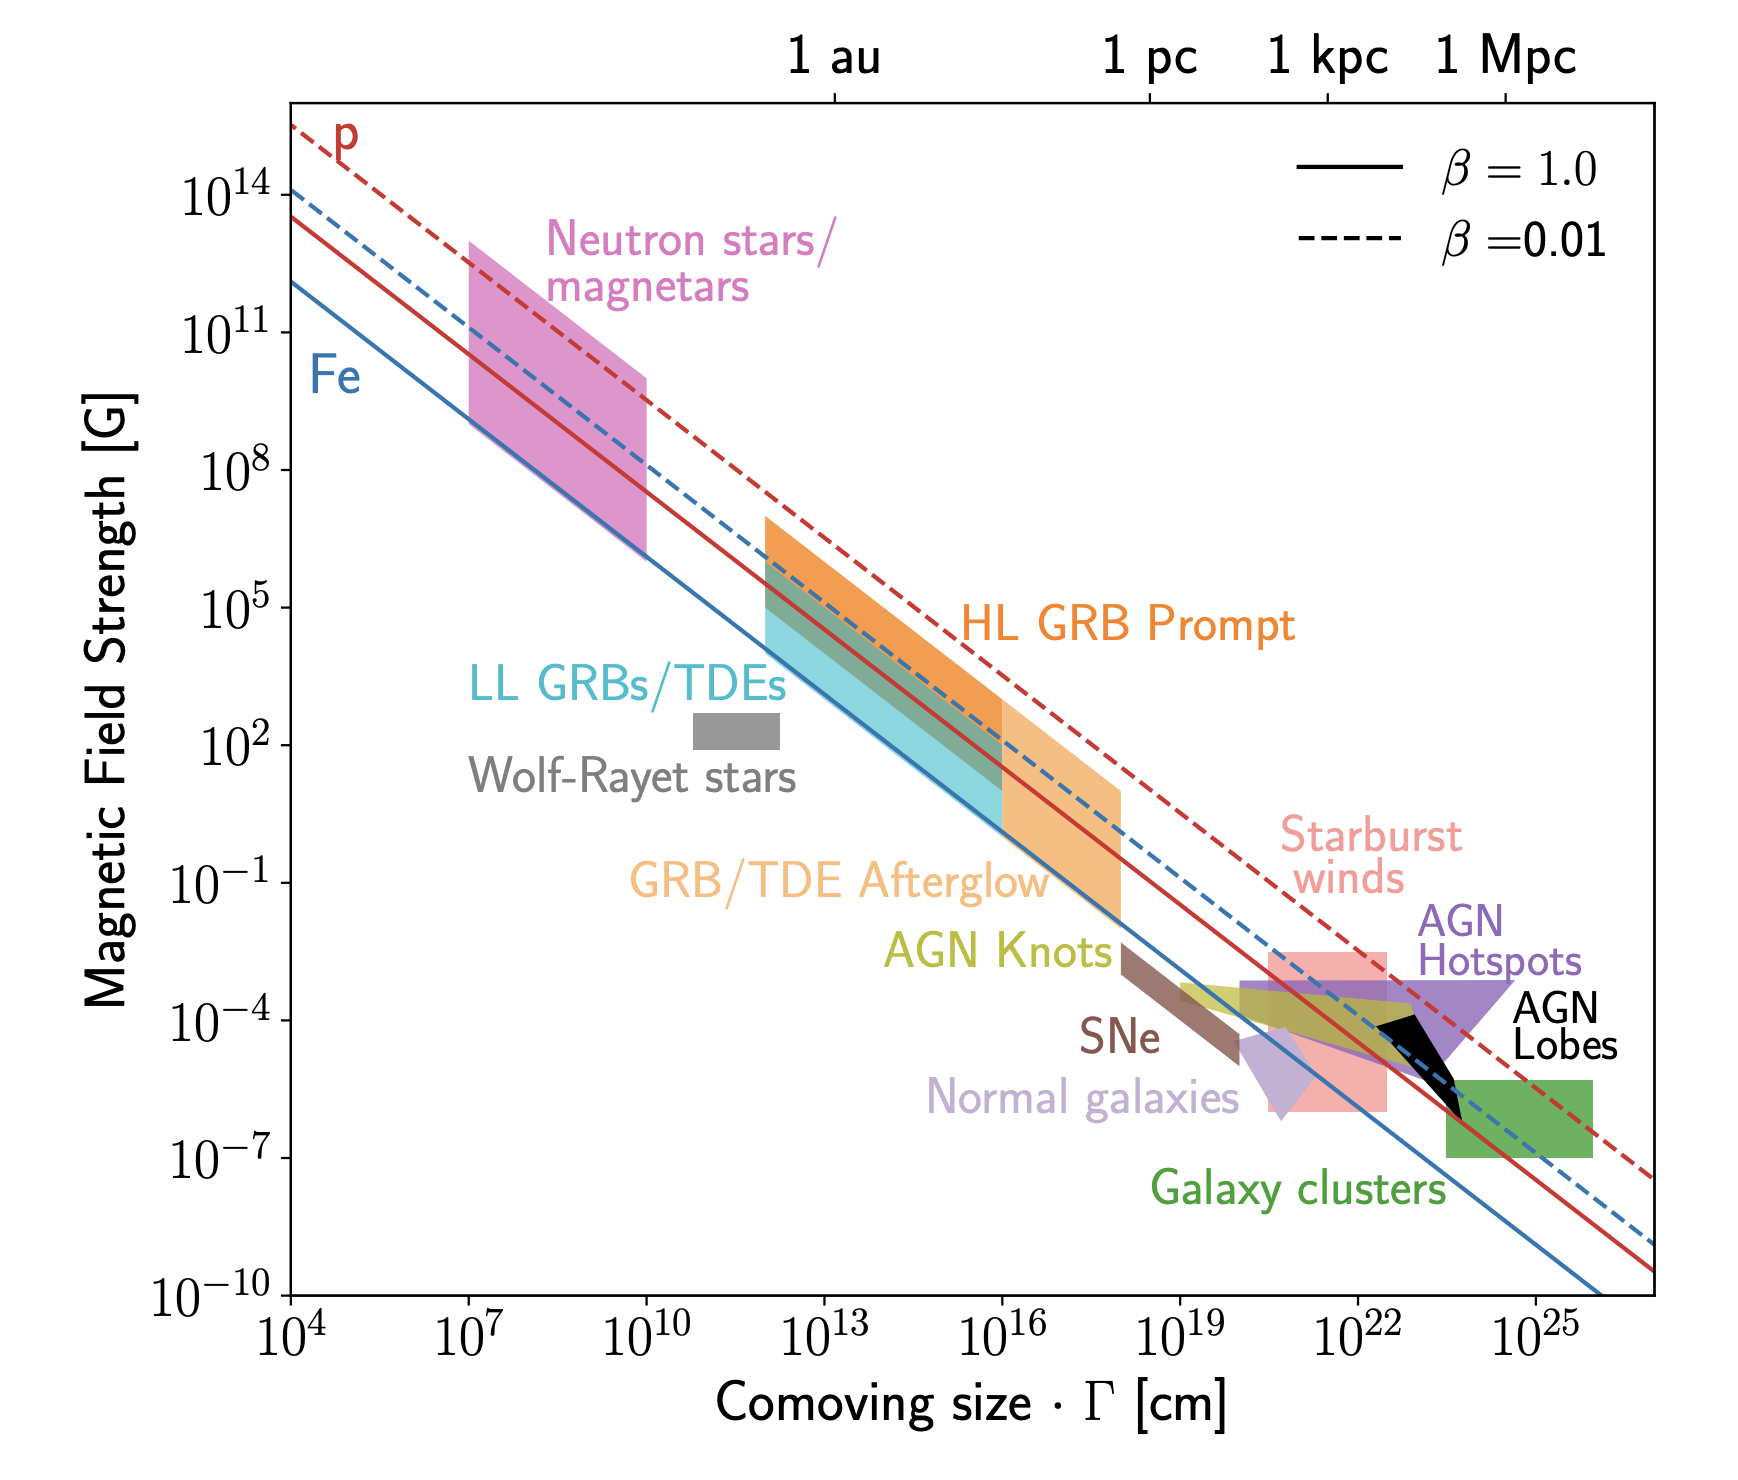
\includegraphics[width=14.5cm]{thesis_figures/CRnNu/Hillas_modified.png}
  \caption{An updated version of Hillas plot. Different source classes are plotted according to their radial size, $R$ (abscissa), and magnetic field strength, $B$. The solid and dashed lines indicate the lower limits above which confinement of protons (red) and iron (blue) nuclei with energy $10^{20}$eV are possible. The solid and dashed lines indicate different shock velocities. Taken from~\cite{AlvesBatista:2019tlv}}.
  \label{fig:Hillas_modified}
\end{figure}


Other accelerating mechanisms are as follows:

1. Supernova Remnants:  Interactions of \glspl{CR} with the magnetic fields within the remnants could lead to further acceleration~\cite{BLASI_2011}.

2. \glspl{AGN}: These are regions in the centre of galaxies that are capable of producing highly energetic particles. The source of this capability is theorized to be powered by supermassive black holes. The extreme conditions near the black holes such as strong magnetic fields and high-energy jets could accelerate \glspl{UHECR}.~\cite{Rieger_2022}

3. Magnetar Outbursts: Magnetars are neutron stars having a magnetic field $\sim$1000 times that of a normal neutron star. They are known to produce magnetically powered bursts which could potentially accelerate particles to \gls{UHECR} level energies.~\cite{PhysRevD.84.023002}

4. Pulsar Wind Nebulae: Rapidly rotating neutron stars, also known as Pulsars emit beams of electromagnetic radiation. Such beams can collide with the ISM creating a pulsar wind nebulae, a region similar to a shock wave front and can lead to production of \glspl{UHECR}.~\cite{Cerutti_2020}

5. Galaxy Clusters: These are regions of galaxy populations bound together by gravity. These highly dense structures can accelerate particles either by themselves or via the shock waves associated with a potential merging of different galaxy clusters.~\cite{Murase_2008,Condorelli_2023} 

6. Relativistic shocks: Other types of astrophysical shocks such as those occurring in gamma-ray bursts or colliding stellar winds could also create scenarios that could accelerate particles to \gls{UHECR} level energies.~\cite{Kirk_2000,10.1046/j.1365-8711.2001.04851.x}

The validity of all such hypothesized mechanisms could be checked by corroborating their spectral index predictions with those observed by the experiments. 

\subsubsection{Top-down scenario}
\label{subsec:Tdownsce}
This is an alternative approach to explaining \glspl{UHECR}. The main idea behind these models is that the \glspl{UHECR} are produced due to the decay or interaction of hypothetical, supermassive, or exotic particles that were produced in the early universe. Some of the proposed hypotheses are mentioned below:

1. Supermassive Dark Matter Particles: This is an extension of a concept that was first proposed to explain dark matter. In this hypothesis, it is assumed that dark matter is composed of long-lived supermassive particles. If such particles exist they could potentially decay and produce \glspl{UHECR}.~\cite{ALOISIO2008307,MARZOLA201756}

2. Cosmic Strings: These are one-dimensional topological defects that could have formed during phase transitions in the early Universe. The decay of these massive strings could also lead to the production of \glspl{UHECR}.~\cite{BHATTACHARJEE2000109,PhysRevD.64.043004}

3. Other Topological effects: These include defects like monopoles or domain walls which could also produce exotic particles which can further decay into \glspl{UHECR}.~\cite{PhysRevLett.79.5202} 

There are other scenarios such as the breakdown of Lorentz invariance which attack the problem of \gls{UHECR} acceleration by suggesting a new mechanism for their production rather than their propagation. Some of these models can be constrained by again looking at the flux of the \glspl{UHECR}~\cite{PierreAuger:2021tog}. There are also experiments that try to directly look for these exotic particles~\cite{XENON:2023cxc,LZ:2022lsv}. So far, no evidence has been found to support the existence of these particles. 

\subsection{Propagation}
\label{subsec:crprop}
Production is just one part of the life of \glspl{CR} or \glspl{UHECR}. To get detected on Earth the \glspl{CR} and \glspl{UHECR} have to travel large distances through ISM during which they can suffer various losses which ultimately affect the spectrum we see on Earth. Some main processes include losses by ionization due to collision with ISM, Synchrotron Radiation which can lead to the emission of high energy photons and, consequently, energy loss for the \gls{CR} particle and through collisions with low-energy photons from radiation fields leading to breakage of CR nuclei also known as Photo-disintegration. Other propagation losses such as Bremsstrahlung and Inverse Compton Scattering due to interactions with the \gls{CMB}, are the reasons high energy \gls{CR} electrons cannot propagate large distances. A few other mechanisms include Adiabatic Energy Loss which affects the energy density due to expansion, Scattering due to magnetic diffusion or even an escape of \glspl{UHECR} from our Galaxy can all affect the spectrum of \glspl{CR} and \glspl{UHECR} we see at Earth. One of the critical phenomena to understand \gls{CR} propagation and to realize a theoretical limit to the energy of \glspl{UHECR} is the \gls{GZK} cutoff. This is discussed in more detail below.

\subsubsection{GZK Limit}
\label{subsubsec:GZK} 
The \gls{GZK} cutoff was first proposed by Kenneth Greisen, an American physicist in 1966 in a paper titled "End to the Cosmic-Ray Spectrum?"~\cite{PhysRevLett.16.748}. He discussed the potential energy loss of high-energy \glspl{CR} due to interactions with the CMB and calculated a threshold energy above which \glspl{CR}, in his case protons, would lose energy through interactions with \gls{CMB}. In the same year, two Soviet physicists, Georgiy Zatsepin and Vadim Kuzmin, arrived at a similar prediction. Their calculations published in their paper "Upper Limit of the Spectrum of Cosmic Rays"~\cite{Zatsepin:1966jv} were consistent with Griesen's work and reinforced the concept of the \gls*{GZK} cutoff.  
The energy cutoff calculated is about 5 x $10^{19}$~\gls{eV} or about 8~joules. The dominant mechanisms via which the proton can interact with the photons of the \gls*{CMB} are given below. 

\begin{equation}\label{eq:GZK}
  \begin{split}
    p + \gamma_{\text{CMB}} &\longrightarrow \Delta^+(1232 ) \longrightarrow n+\pi^+ \\ 
                     &\longrightarrow \Delta^+(1232 ) \longrightarrow p+\pi^0
  \end{split} 
  \qquad
  \begin{split}
    N + \gamma_{\text{CMB}} &\longrightarrow N' + \pi^{\pm} \\ 
                     &\longrightarrow N' + \pi^0 \, , 
  \end{split} 
\end{equation}
where N is the nucleon involved in the interaction and N' is the final state nucleon which could be same or different depending on the initial nucleon. These processes are also called "Photo-pion Production". The thresholds for these reactions or the energy of the photon are of the order of $\sim$a few hundred Megaelectron volt (MeV = $10^6$eV) for protons and a few gigaelectron volt (GeV = $10^9$eV) per nucleon for other nuclei in the rest frame of the proton and nucleon respectively. In the context of the CMB which have an E $\sim 10^{-4}$eV, the predicted cutoff for protons is 50 Exa-electron-volt (EeV = $10^{18}$eV) whereas for heavy nuclei it can range from about 80 EeV to several hundred EeV depending on the mass of the incident nucleus in the lab frame (relevant for astrophysical observations). The mean free path which represents the average distance a \gls{CR} particle can travel before undergoing a significant interaction depends on the initial energy, interaction crossection and the number density of target photons. For a UHE protons interacting with the CMB photon, the mean free path is about $\sim$50-100 Mpc. This leads to the outcome that if a \gls{UHE} proton with energy above the GZK cutoff travels over a distance larger than 50Mpc then such a proton will suffer catastrophic losses and will not be observed in the UHE regime. However, this consequence doesn't hold for heavy nuclei since for similar energies Photo-pion production is not the dominant process via which they can lose energy. For \glspl{UHECR} composed of heavy nuclei (e.g., iron, uranium), the dominant energy loss process during their propagation through the universe is photo-disintegration. It can be described as:
\begin{equation}\label{eq:Pdisinteg}
  \begin{aligned}
    p + \gamma_{\text{CMB}} &\longrightarrow n + \pi^+ \\
    (A,Z) + \gamma_{\text{CMB}} &\longrightarrow (A-n, Z- n') + nN ,  
  \end{aligned} 
\end{equation}
with $n\,(n')$ being the number of stripped nucleons (protons). The mean free path for photo-disintegration for a photon field such as the CMB is similar to that of photo-pion production. Even though, the Pierre Auger Observatory observes a suppression in the \gls{CR} spectrum above the \gls{GZK} cutoff~\cite{KAMPERT2014318}, it does not claim it to be just due to GZK limit. It has also observed \glspl{CR} above the \gls*{GZK} cutoff. This issue along with its implications is discussed later in section~\ref{subsubsec:CRspectrum}. One of the other consequences arising from the interaction with the CMB is the interaction of ultra high energy photons (UHE$\gamma$s, E > $10^{16}$eV) to produce electron-positron pairs, $\gamma_{\text{UHE}} + \gamma_{\text{CMB}} \longrightarrow e^+ + e^- $. This is an important consequence that alters both the expected \gls{UHECR} spectrum and the CR spectrum at Earth and also just leaves neutrinos as one of the few known UHE particles that can point back directly to their sources over long distances.

The production of these high energy neutrinos arising from the pions produced during the Photo-pion interaction or via the neutrons produced during photo-disintegration is discussed later in section~\ref{sec:UHENu}. 

\subsection{Latest results}
\label{subsec:CRresults}
The study of \glspl{CR} to constrain their properties and the relevant sources requires measurements at Earth. The measurements which provide valuable information are the energy spectrum or flux observed at Earth, the composition of the primary \glspl{CR}, their arrival direction and other relevant observations such as measurement of other messengers like as high energy photons and neutrons. These measurements and their implications are discussed in more detail below. The high energy neutrinos, relevant for this thesis are discussed in a separate section. 

\begin{figure}[t!]
  \centering
  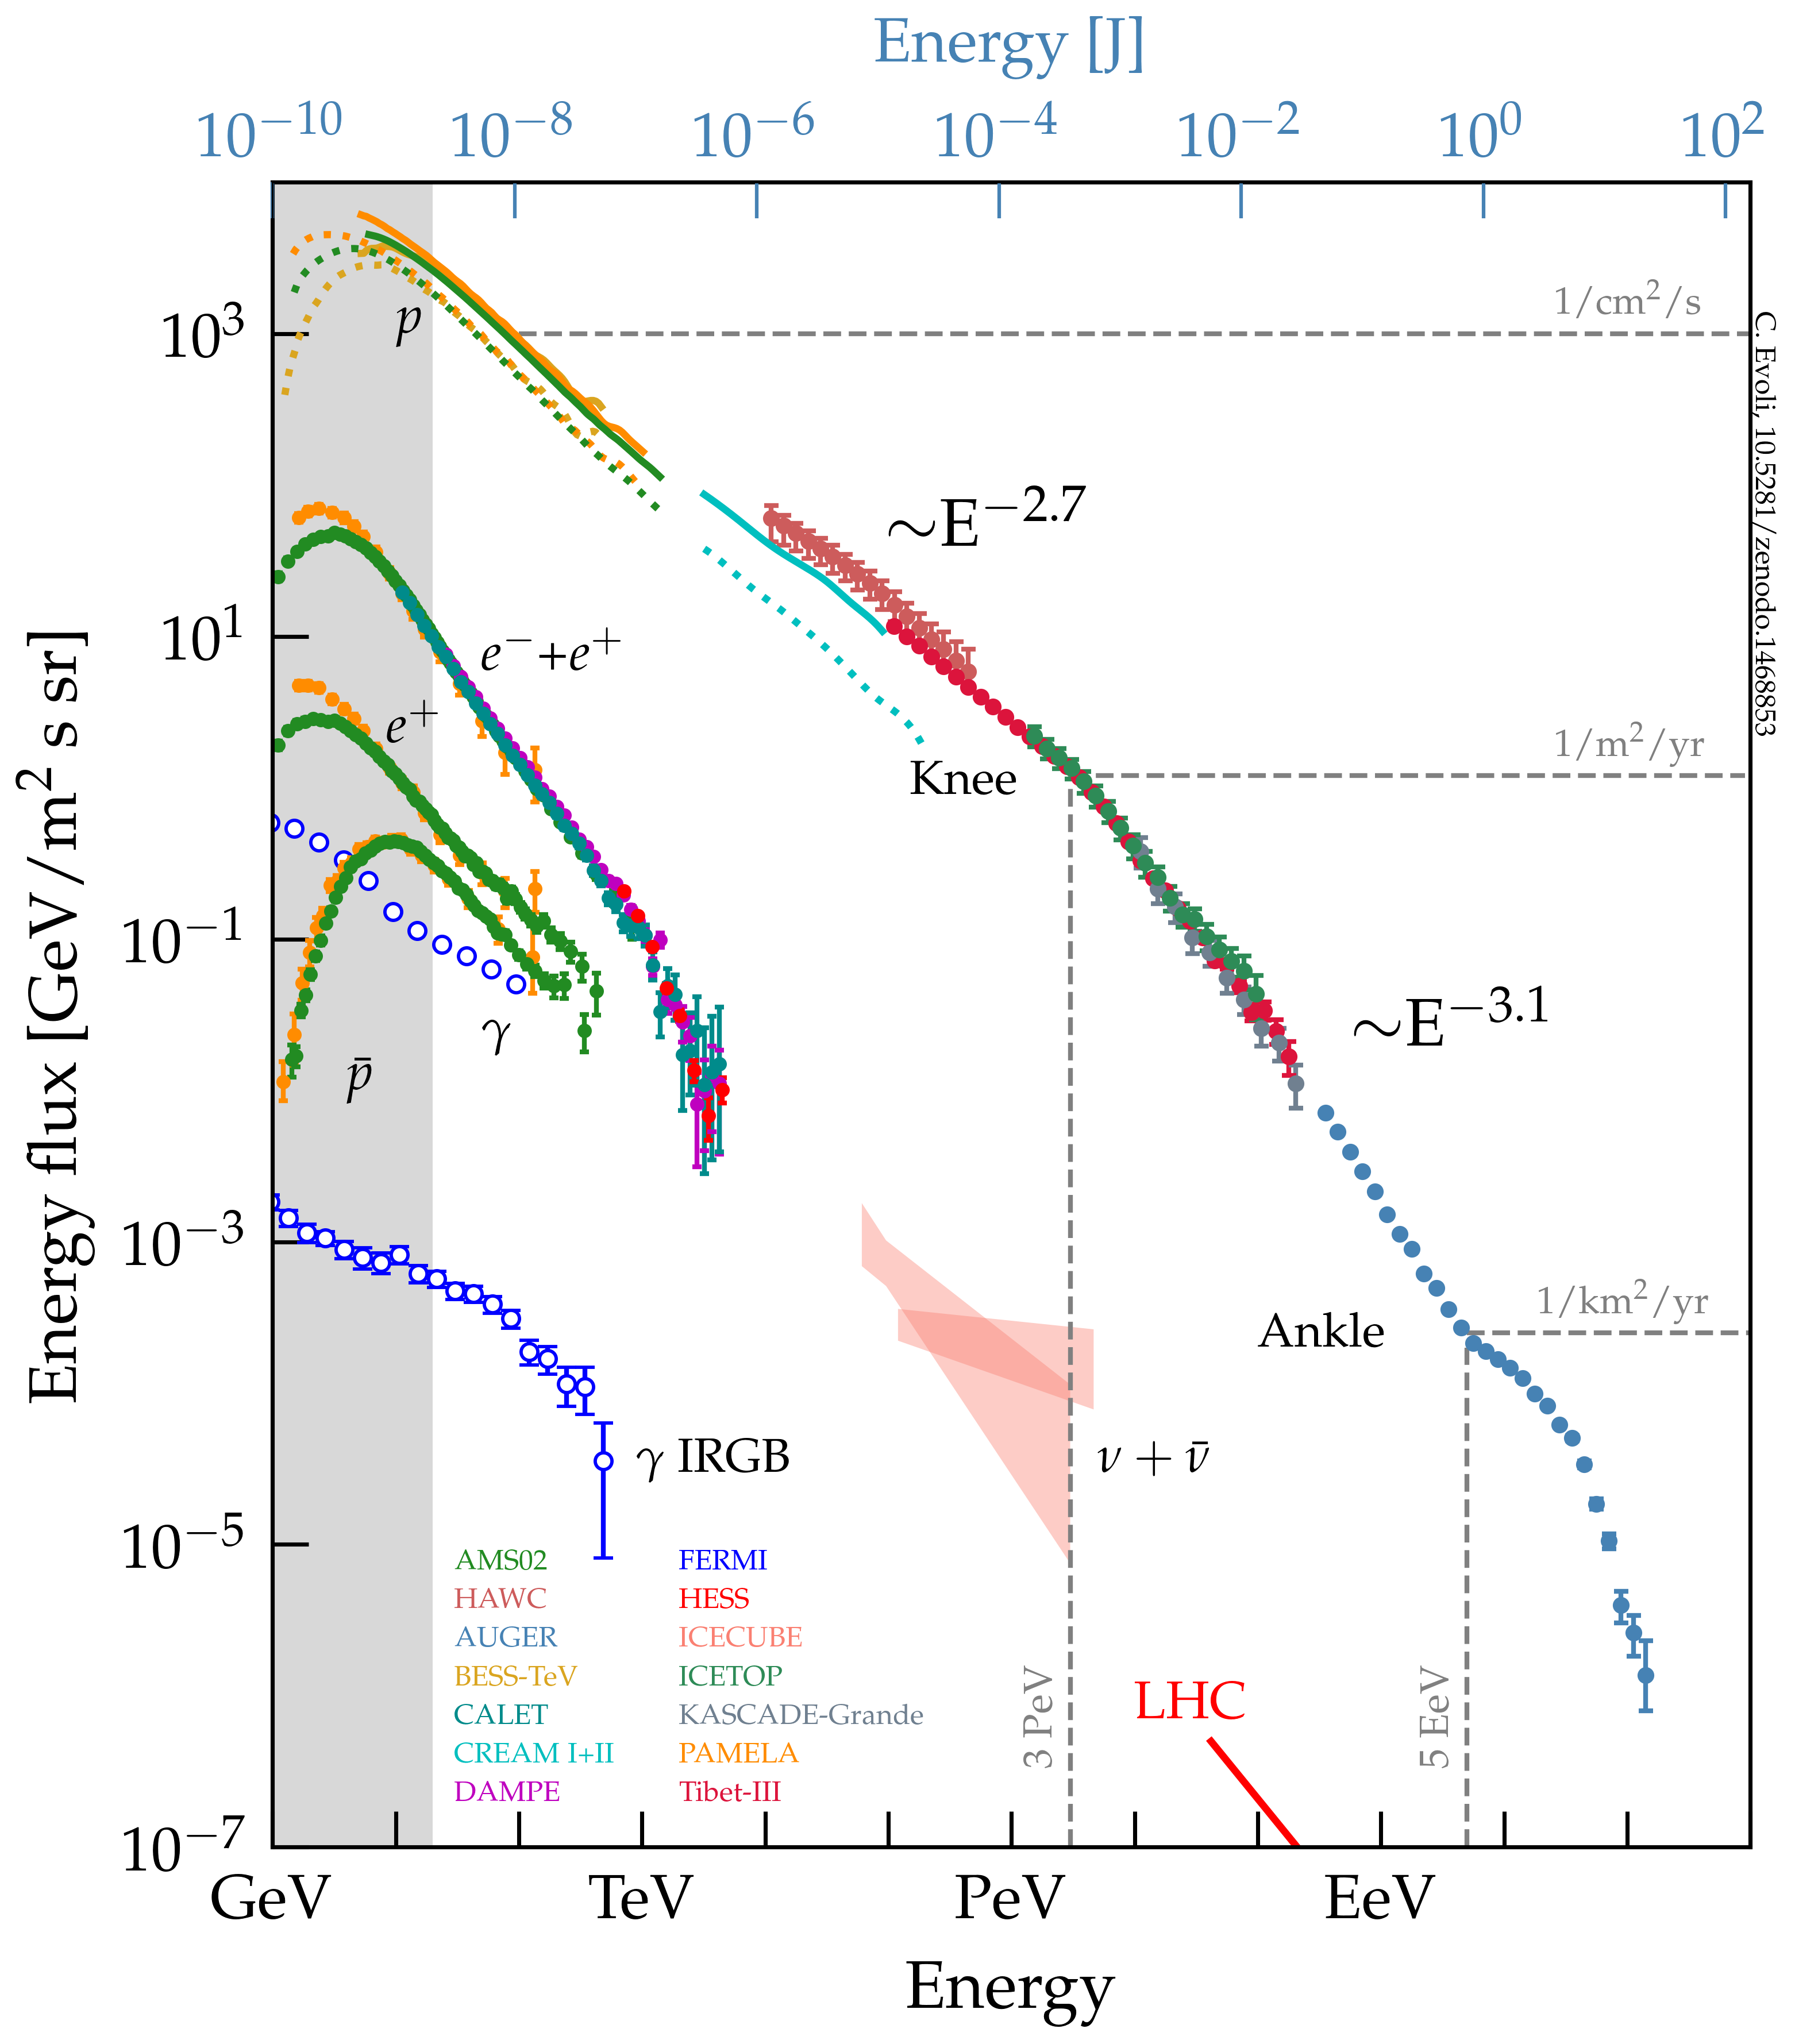
\includegraphics[width=14.5cm]{thesis_figures/CRnNu/all_particle_spectrum.png}
  \caption{Cosmic flux vs Energy spectrum. The colour indicates the experiment used to record the flux. At lower energies we have much detailed information about the composition. At high energies only the all particle spectrum is shown due to low flux. Also shown is the gamma ray spectrum recorded by FERMI and the neutrino flux measurement by IceCube. Taken from~\cite{evoli_2018_2360277}}.
  \label{fig:CR-spectrum}
\end{figure}
\subsubsection*{Cosmic Ray spectrum}
\label{subsubsec:CRspectrum}
The \gls{CR} spectrum measured by several experiments on Earth is summarized in Fig.~\ref{fig:CR-spectrum}. Extending in energy from a few 100 MeV (solar \glspl{CR}) it spans about 12 orders of magnitude up to the most energetic observed \glspl{CR} above $10^{20}$eV. The flux decreases with increasing energy and follows a varying power law description:

\begin{equation}
  \label{eq:Powlaw}
  \frac{dN}{dE} \propto E^{-\gamma},   
\end{equation}
where $\gamma$ is the spectral index. The spectral index varies between 2.7 to 3.3 as measurements are made for higher energies. This signifies a decrease in the observed flux as the energy increases. The flux falls from $\mathrm{\sim 1m^{-2} s^{-1}}$ at $10^{11}$eV to $\mathrm{\sim 1m^{-2} yr^{-1}}$ at $10^{16}$eV to about $\mathrm{\sim 1km^{-2} yr^{-1}}$ at $10^{19}$eV. Such a steep fall also poses challenges for the experimental design and the corresponding size. This further affects the detection mechanisms employed to measure this spectrum, due to the very low flux expected at high energies, the measurements of the direct primaries become nearly impossible and an indirect detection using the property of the \gls{CR} to trigger an air shower in our atmosphere is employed. This phenomenon and how it is used to measure \glspl{CR} is discussed in the next chapter~\ref{chap:EAS}.

% \begin{figure}[t!]
%   \centering
%   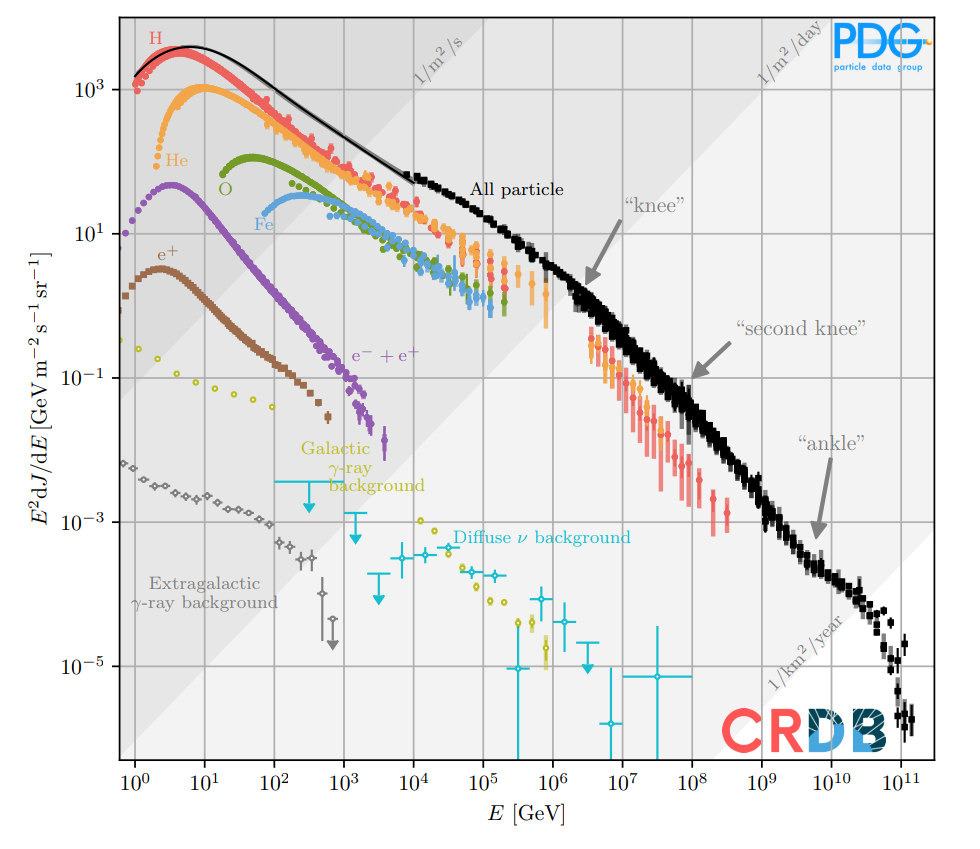
\includegraphics[width=14.5cm]{thesis_figures/CRnNu/CR-spectrum.png}
%   \caption{Spectrum PDG, CRDB~\cite{ParticleDataGroup:2024cfk} (Which figure is better ?)}
%   \label{fig:CR-spectrum_scaled}
% \end{figure}

% To better deduce the features in the \gls{CR} spectrum one can scale the flux in the fig~\ref{fig:CR-spectrum} by energy. The corresponding figure is shown in fig.~\ref{fig:CR-spectrum_scaled}. 
Below $10^{13}$eV \glspl{CR} from the Sun dominate the spectrum. The galactic or extragalactic \glspl{CR} of these energies cannot enter our solar system because of a variety of reasons. These include a combination of the Heliosphere, termination shock and solar modulation which block the low energy \glspl{CR}. The Heliosphere which is a region influenced by the Sun's magnetic field and solar wind acts as a protective bubble around the solar system. Beyond the Heliosphere, the solar wind interacts with the ISM creating a region of termination shock which can cause scattering and deflection for incoming low energy \glspl{CR}. Additionally, the solar activity cycle can cause changes to the Heliosphere which in turn also affects the incoming \glspl{CR}. Beyond a few GeVs the Sun as a source of \glspl{CR} drops off due to reaching its maximum acceleration potential. Between $10^{13}$eV and $10^{18}$eV the spectrum is dominated by \glspl{CR} of galactic origin. This has been verified by comparing the spectral indices of the proposed acceleration mechanisms with the measured spectrum as mentioned before. A second proof also comes from the composition of the \glspl{CR} observed in these energies, but this is discussed later. \textit{Supernovae} and \textit{supernovae remnants} remain the most promising sources which could explain their origin. The spectral index, $\gamma \sim$ 2.7 gives a good description of this region. Around $\sim5 \times 10^{15}$ one observes a steepening of the spectrum known as the \textit{knee}. At this point $\gamma$ changes from 2.7 to 3.1. This is attributed to the galactic accelerators reaching their maximum potential for accelerating protons. Above the knee, the sources are expected to reach their maximum potential for other heavier particles until galactic sources cannot accelerate \glspl{CR} any further. This point is thought to be the origin of the second knee at $\sim 10^{17}$eV. At this point the $\gamma$ changes from 3.1 to 3.3. This is theorized to be a transition region in which the spectrum is believed to change from one of galactic origin to extragalactic origin. This region ends at about $\sim 10^{18}$eV whereon the spectrum hardens noticeably to a $\gamma \sim$ 2.6, originating what is referred to as the \textit{ankle}. Further, with increasing energy the spectrum again steepens to $\gamma \sim$ 5.1 reaching an eventual cutoff. The suppression of flux at these energies and the cutoff is still not properly understood yet and could be due to the following possibilities:

1. \textbf{GZK Limit:} One of the most prevalent ideas behind the suppression and the cutoff is the GZK mechanism which was discussed above. Due to the observations of \glspl{CR} above the cutoff of $\sim 10^{18.5}$eV by the Pierre Auger Observatory and a non-observance of expected composition (non-proton primaries) and neutrino flux (GZK pion decay), GZK as the only reason for the observed cutoff in the spectrum is currently disfavoured. However, tensions between the composition measurements of the Pierre Auger Observatory and the \gls{TA}~\cite{kawai2008telescope}, the second-largest \gls*{CR} observatory, make this topic still a subject of debate.

2. \textbf{Maximum Rigidity:} In this scenario, the cutoff is due to the sources of the extragalactic \glspl{CR} reaching their maximum potential for acceleration for different particles i.e. maximum rigidity. Such a scenario is already observed in the spectrum for Galactic sources (\textit{knee}). An indirect proof of this mechanism can come from the observed composition from the \textit{ankle} region to the cutoff. If the composition shifts from lighter to heavier nuclei this would be proof of a cutoff at the potential extragalactic sources. 

3. \textbf{Photo-disintegration:} This effect was also discussed before in section~\ref{subsubsec:GZK}. However, for such a scenario the cutoff would appear in steps depending on the mass of the nuclei. 

It is likely that the cutoff and the suppression are not just because of one of the above-mentioned scenarios but are due to a combination of all three. In theory, \gls{GZK} and Photo-disintegration could explain the observed spectrum but the non-observance of \gls*{GZK} neutrinos and the composition measurements gather otherwise. It also shows that even though the CR spectrum gives a very nice overview, other crucial measurements of composition and multi-messengers are equally important allies to the spectrum measurements for constraining the origin and propagation of \glspl{CR}.

\subsubsection*{Cosmic Ray composition}
\label{subsubsec:CRcompo}
The types of particles the \gls{CR} flux at Earth is made of is called the \gls*{CR} composition. Such measurements with respect to energy offer a very useful insight into their origin. Direct measurement of the primaries is only possible for low energies and one e.g. is the AMS detector at the International Space Station~\cite{PhysRevLett.110.141102}. For higher energies, the mass of the primary is reconstructed by measuring the phenomenon of \glspl{EAS} which is described in more detail in Chapter~\ref{chap:EAS}. \glspl*{EAS} are created when high-energy \glspl{CR} interact with the Earth's atmosphere producing a cascade of particles resembling a shower.  Depending on the mass of the primary, the \gls{EAS} induced in the atmosphere by the said primary has characteristic differences. For the same energy lighter nuclei such as protons will interact and produce an \gls{EAS} much deeper in the atmosphere compared to heavy nuclei such as iron. There are various ways one could estimate the mass of the primary. The estimator used for this at the Pierre Auger Observatory is <$X_{\text{max}}$> which is the average depth at which the \gls{EAS} development in the atmosphere reaches a maximum. The <$X_{\text{max}}$> values are also energy dependent, and it is observed that iron nuclei typically have values $\sim$100 g cm$^{-2}$ lower than proton. The fluctuation in the spread, $\sigma<X_{\text{max}}>$, can also be used to gauge the mass. For example, fewer fluctuations are expected for iron compared to proton. Other quantities such as the lateral distribution of the shower which is just the number of particles in a shower as a function of distance from the line along the CR momentum (shower core) also shows differences based on the primaries. For lighter primaries, the distribution is broader i.e. the number of particles decreases more gradually with distance from the core compared to a narrower distribution in the case of heavier primaries. The ratio of electromagnetic to muonic components first used by KASCADE~\cite{SCHATZ1998151} can also be used to differentiate between the primaries, the lighter primaries have a greater electromagnetic component whereas the heavier primaries have a greater muonic component in the initiated EAS.    

\begin{figure}[t!]
  \centering
  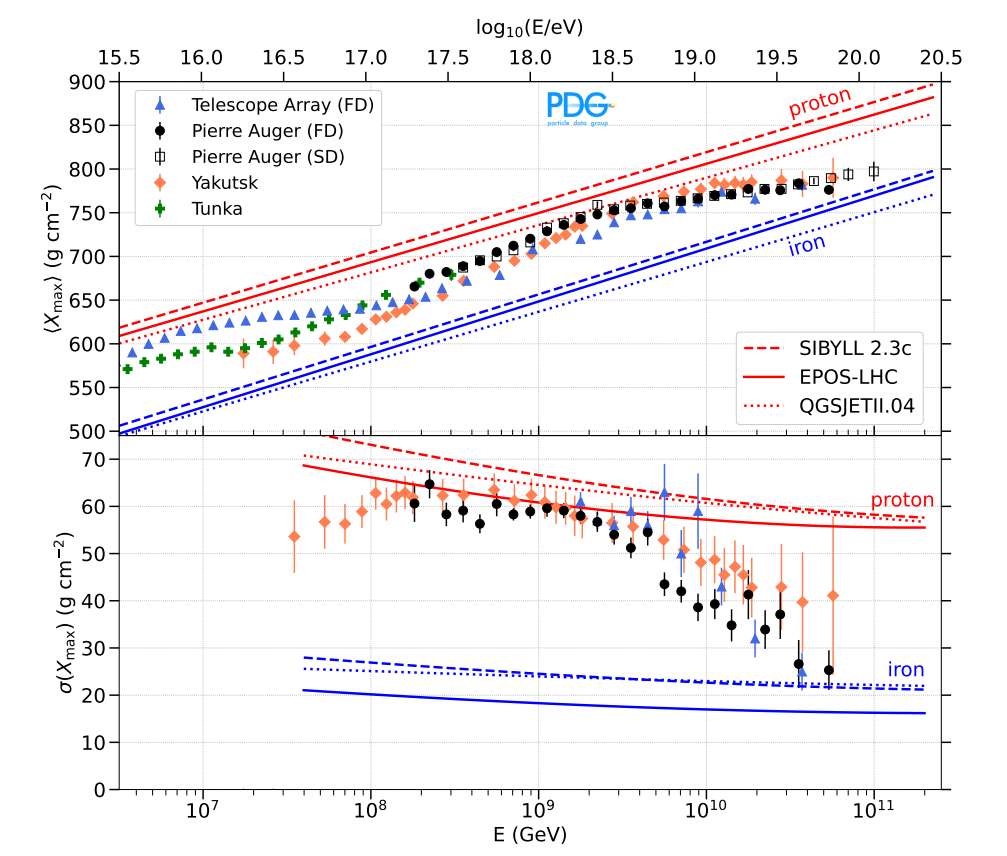
\includegraphics[width=14.5cm]{thesis_figures/CRnNu/Composition_measurement.png}
  \caption{Measurements of mass composition by different experiments. $<X_{\text{max}}>$ (top) and its fluctuations $\sigma<X_{\text{max}}>$ (bottom). The red and blue lines are obtained from simulations with different hadronic interaction models. Taken from~\cite{ParticleDataGroup:2024cfk}}.
  \label{fig:CR-composition}
\end{figure}

The process of estimating the mass requires a very robust simulation that can reconstruct an EAS perfectly for a certain primary and a direct observation of $X_{\text{max}}$. At the Pierre Auger Observatory The \gls{FD}, cf. section~\ref{sec:Fl_det}, is used to directly measure the $X_{\text{max}}$ on an event by event basis. The recent results from the Pierre Auger Observatory are shown in Fig.~\ref{fig:CR-composition}. In both the figures the composition initially turns lighter and then seems to change from lighter to heavier nuclei at E $\sim$18.5 EeV. This could be an indication of the switch from a galactic component to an extragalactic component around the \textit{ankle} consistent with the maximum rigidity scenario as mentioned in the section above.

However, the duty cycle of the \gls{FD}$\sim$14\% compared to the \gls{SD} $\sim$100\% leads to very limited statistics. Currently, this problem is solved by defining a new observable described in~\cite{2017arXiv171007249T} which has helped increase the number of events used to estimate the mass composition by nearly 14 times. The results for this are also shown in Fig.~\ref{fig:CR-composition}. Additionally, the energy dependent mass composition can be fitted simultaneously with the \gls{CR} spectrum observed at the Pierre Auger Observatory with the only required assumption being about the model used to produce and propagate the \glspl{CR} from the sources. Such type of analysis performed at the Pierre Auger Observatory can be found in~\cite{2018_auger_comp_spec}. With the current Pierre Auger Observatory measurements four different mass components are required to best describe the data with proton component completely disfavoured for the highest energies.

The future advancements of the AugerPrime~\cite{ANASTASI2022167497} will further increase the capability of the Pierre Auger Observatory in measuring mass composition. The addition of a Radio Detector can present an independent measurement of the $X_{\text{max}}$ offering an important cross-check on the \gls{FD} measurement. 

\subsubsection*{Cosmic Ray arrival directions}
\label{subsubsec:CRdirec}
\begin{figure}[t!]
  \centering
  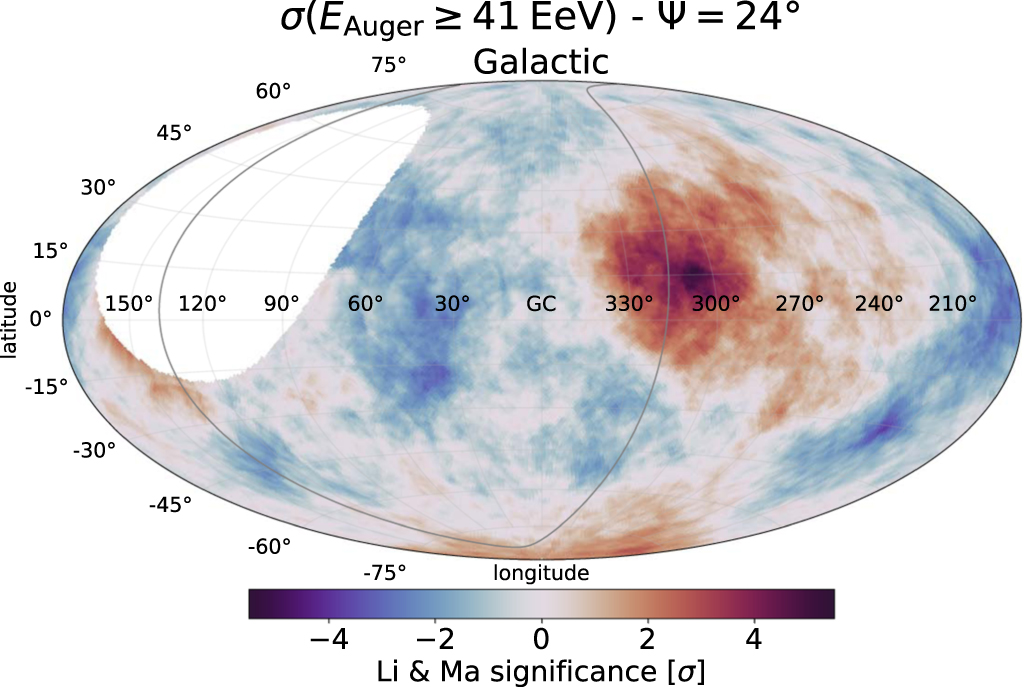
\includegraphics[width=14.5cm]{thesis_figures/CRnNu/apjac7d4ef1_hr.jpg}
  \caption{Localized excess or Li-Ma~\cite{Li:1983fv} significance map at energies above 41 EeV and within a top-hat search angle $\Psi = 24^\circ$ in Galactic coordinates. The gray line indicates the super galactic plane. Area outside the field of view of the Observatory is shown in white. The dark red areas indicate the possible source locations of extragalactic \glspl{UHECR}. Taken from~\cite{Abreu_2022}}.
  \label{fig:CR-anisotropy}
\end{figure}

Even though the \glspl{CR} are mostly charged particles and can easily get deflected by the magnetic fields~\cite{Ar_mburo_Garc_a_2021} present in the cosmos one can still estimate the arrival directions of these \glspl{CR} with the help of a good pointing resolution and an understanding of these magnetic fields. The pointing resolution depends on the detector and the Pierre Auger Observatory already has an excellent pointing accuracy of $\sim 0.7^{\circ}$~\cite{BONIFAZI200920}. The magnetic fields on the other hand are complicated to deduce and model. However, this lack of knowledge can be ignored by just looking at \glspl{CR} of high energies since the expected deflections for such \glspl{CR} are expected to be small. At the Pierre Auger Observatory the arrival directions of more than 2,600 \glspl{CR} above 32EeV were estimated and analysed to look for potential sources of these \glspl{CR}~\cite{Abreu_2022}. The most significant result from this study is shown in Fig.~\ref{fig:CR-anisotropy}. The figure clearly shows the presence of anisotropies which are deviations from uniformity across the sky. The anisotropies are also pointed away from the Galactic centre indicating that the \glspl{UHECR} have an extragalactic origin. The hypothesis is further confirmed by the increase in anisotropy with energy shown in~\cite{Abreu_2022}. The presence of these anisotropies not far from the Galactic spiral arm as seen in Fig.~\ref{fig:CR-anisotropy} also gives further proof of an extragalactic origin of these \glspl{UHECR}. Further, for low energies E> 0.03 EeV studies looking at large scale structures such as dipolar flux modulation in~\cite{Aab_2020_dipole_modulation} also show a shift of the anisotropy dipole more towards the galactic centre with decreasing energy with a significance of $\sim 6 \sigma$. This can again be interpreted as a transition in CR sources from Galactic to extragalactic component. Even though this result is corroborated by the measurements done by KASCADE-Grande, IceCube and IceTop due to the decrease in sensitivity of the Pierre Auger experiment for these energies the result is not conclusive yet.

Some proposed sources for these \glspl{UHECR} due to observations of excess \glspl{UHECR} in their surrounding regions by the Pierre Auger Observatory are presented in~\cite{TelescopeArray:2021gxg}. These include the Centaurus A region ($\sim 4\sigma$ significance), starburst galaxies ($\sim 3.8\sigma$) such as NGC4945, M83 and NGC253. The \gls{TA} has also found an excess close to the Perseus-Pisces supercluster with a significance of $\sim3.0-3.2\sigma$. However, this is still unconfirmed by the Pierre Auger Observatory which can also partly observe supercluster and remains a topic of discussion. With the continued data taking and upgrade of the Pierre Auger Observatory, the excess in the Centaurus A region is expected to reach a significance of 5$\sigma$  by 2025 which could make it the first steady source of \glspl{UHECR} ever observed. 
 

\subsubsection*{Other Messengers}
\label{subsubsec:CRmessengers}
The scenarios for the production and propagation of \glspl{CR} discussed above also predict the production of other messengers such as photons, neutrinos and neutrons. Neutrons and photons are discussed in this section and neutrinos are discussed in the next. 
Neutrons being neutral and thus not affected by the magnetic fields of the Universe during their propagation can be useful for arrival direction studies. They are expected to be produced at the CR source via photo-pion production or other nuclear reactions near the sources. One such e.g. is a collision between an ultra-high energy proton to an ambient proton/photon. Although, neutrons can lose a significant amount of their acquired energy very quickly via $\beta$ decay (mean lifetime$\sim$879\,s)~\cite{ParticleDataGroup:2024cfk} in the ultra-relativistic regime neutrons originated in our Galaxy can still make it to Earth. At Auger, a neutron produces a non-distinguishable EAS as compared to a proton. Hence, only a source catalogue correlated search can be performed at the Pierre Auger Observatory. The results of such a search are given in~\cite{PierreAuger:2023onx}. No neutron like events have been found at Auger, but these results have already helped constrain some theorized production mechanisms for \glspl{CR}. Future searches looking at transient or short-lived sources for neutrons are currently underway. 

Photons again offer another window to look into the origin, propagation and sources of the \glspl*{CR}. They can either be produced via interactions of \glspl*{CR} with matter or radiation fields or during propagation through interactions with the \gls*{CMB} as mentioned in section~\ref{subsec:crprop}. They, along with neutrinos, can also help constrain various top-down scenarios and help paint a more complete picture of the CR landscape. Observations for high energy photons have been carried out by specialized experiments such as ground-based Cherenkov telescopes like the \gls{HESS}~\cite{Puhlhofer:2024fjx}, Fermi Gamma-ray Space Telescope~\cite{Thompson_2022}, and the upcoming \gls{CTA}~\cite{2018_CTAO}. The Pierre Auger Observatory can also contribute to this search in the ultra-high energy regime by looking for photon-induced EAS. Such EASs are expected to be different from the ones induced by \glspl{CR} as they have a larger electromagnetic component and a rather small hadronic component. A more detailed description of the signature is provided in~\cite{universe8110579}. 

\begin{figure}[t!]
  \centering
  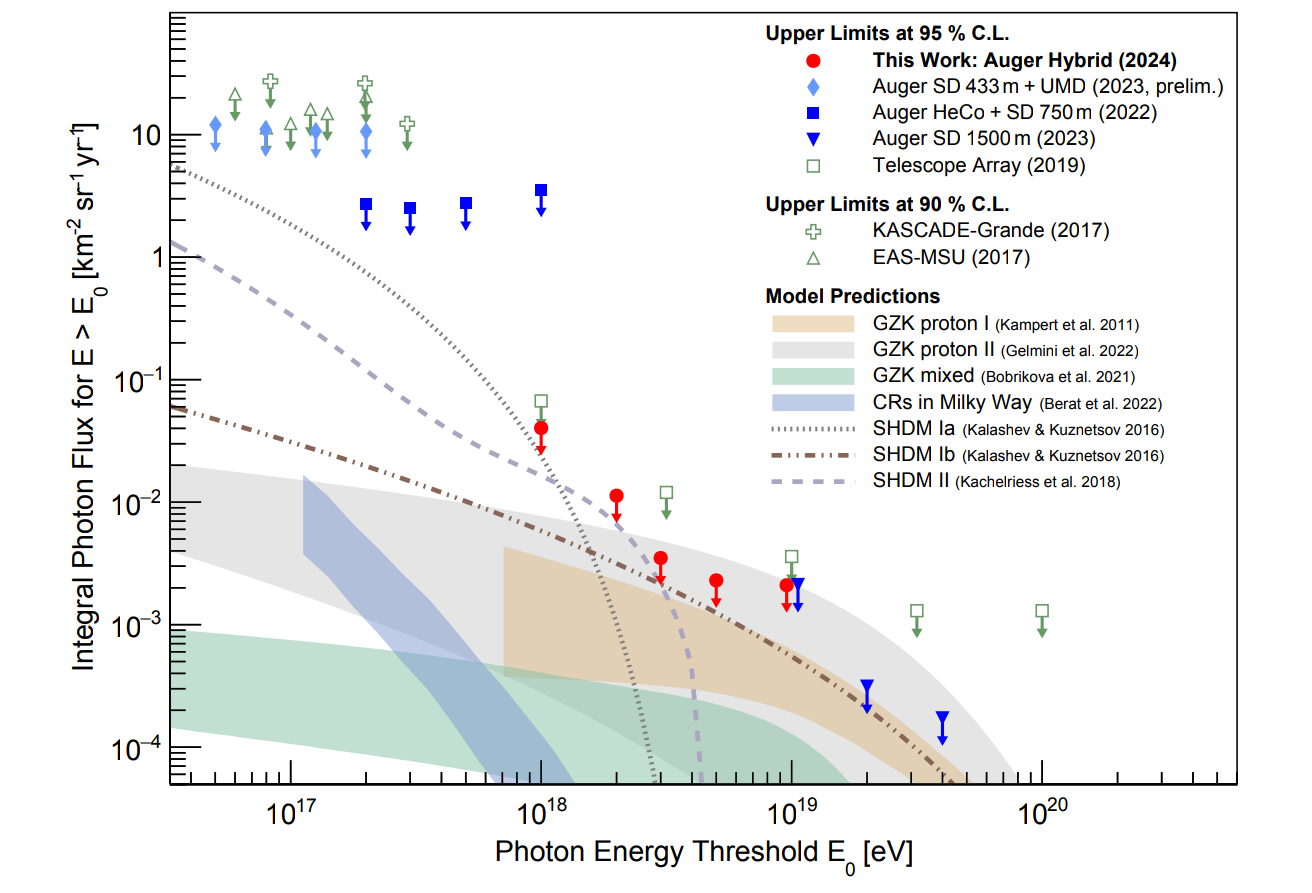
\includegraphics[width=14.5cm]{thesis_figures/CRnNu/Photon-limits.png}
  \caption{Summary of the current upper limits on the integral photon flux determined by Pierre Auger Observatory and other experiments~\cite{PierreAuger:2024ayl}}.
  \label{fig:Auger-Photon-limits}
\end{figure}

Summary of the results of photon searches performed at the Pierre Auger Observatory is presented in Fig.~\ref{fig:Auger-Photon-limits} together with the predicted flux from some popular production models. Due to the non-observance of photon-like events at Auger, the collaboration has set some of the stringiest limits for expected photon flux at high energies. This has already helped constrain some top-down scenarios ultimately leading to a much better understanding of the origin of \glspl{UHECR}. Further, searches will also help constrain the mystery of the cutoff. UHE photon searches are also very useful for a multimessenger approach to astronomy and these contributions are discussed more in section~\ref{sec:Mul-mes}.


\section{Ultra High Energy Neutrinos}
\label{sec:UHENu}
\subsection{History}
Neutrino ($\nu$)~\cite{10.1063/1.2995181} (neut-neutral, ino-small) is an elementary particle belonging to the fermion class with a 1/2 spin. It was named by Enrico Fermi but first postulated by Pauli in 1930 as an explanation for the conservation of energy, momentum and angular momentum in $\beta$ decays. It rarely reacts in nature and only scatters via weak interaction. The neutrino was first observed in 1956 by the Cowan-Reines neutrino experiment~\cite{PhysRev.92.830} by detecting the positron annihilation of neutrons and positrons produced by antineutrinos created in a nuclear reactor. Neutrinos can have three flavours electron neutrinos ($\nu_e$), muon neutrinos ($\nu_{\mu}$), or tau neutrinos ($\nu_{\tau}$) depending on the charged lepton (electron, muon or tau) accompanying them in their production. There are various mysteries involved with understanding this "ghost particle". One of these is the phenomenon of neutrino oscillations which is the intermixing of different neutrino flavors as they propagate through space. This has been observed in various experiments such as the Super-Kamiokande Observatory~\cite{Fukuda_1998} and the Sudbury Neutrino Observatories~\cite{BELLERIVE201630} and was the recipient of the 2015 Nobel Prize for Physics since it was the first indication that neutrinos have some mass. This has led to various efforts to determine the mass of the three neutrinos (under Neutrino Properties in~\cite{ParticleDataGroup:2024cfk}). Currently, only a hierarchical differentiation can be established~\cite{Qian_2015}, the configuration of which is also not completely understood, and further experiments like Karlsruhe Tritium Neutrino experiment~\cite{aker2024directneutrinomassmeasurementbased} are underway to solve this mystery. Also, the very mechanisms with which neutrinos can acquire mass are currently not completely understood~\cite{CERN_courier_nu_mass}. 
\begin{figure}[t!]
  \centering
  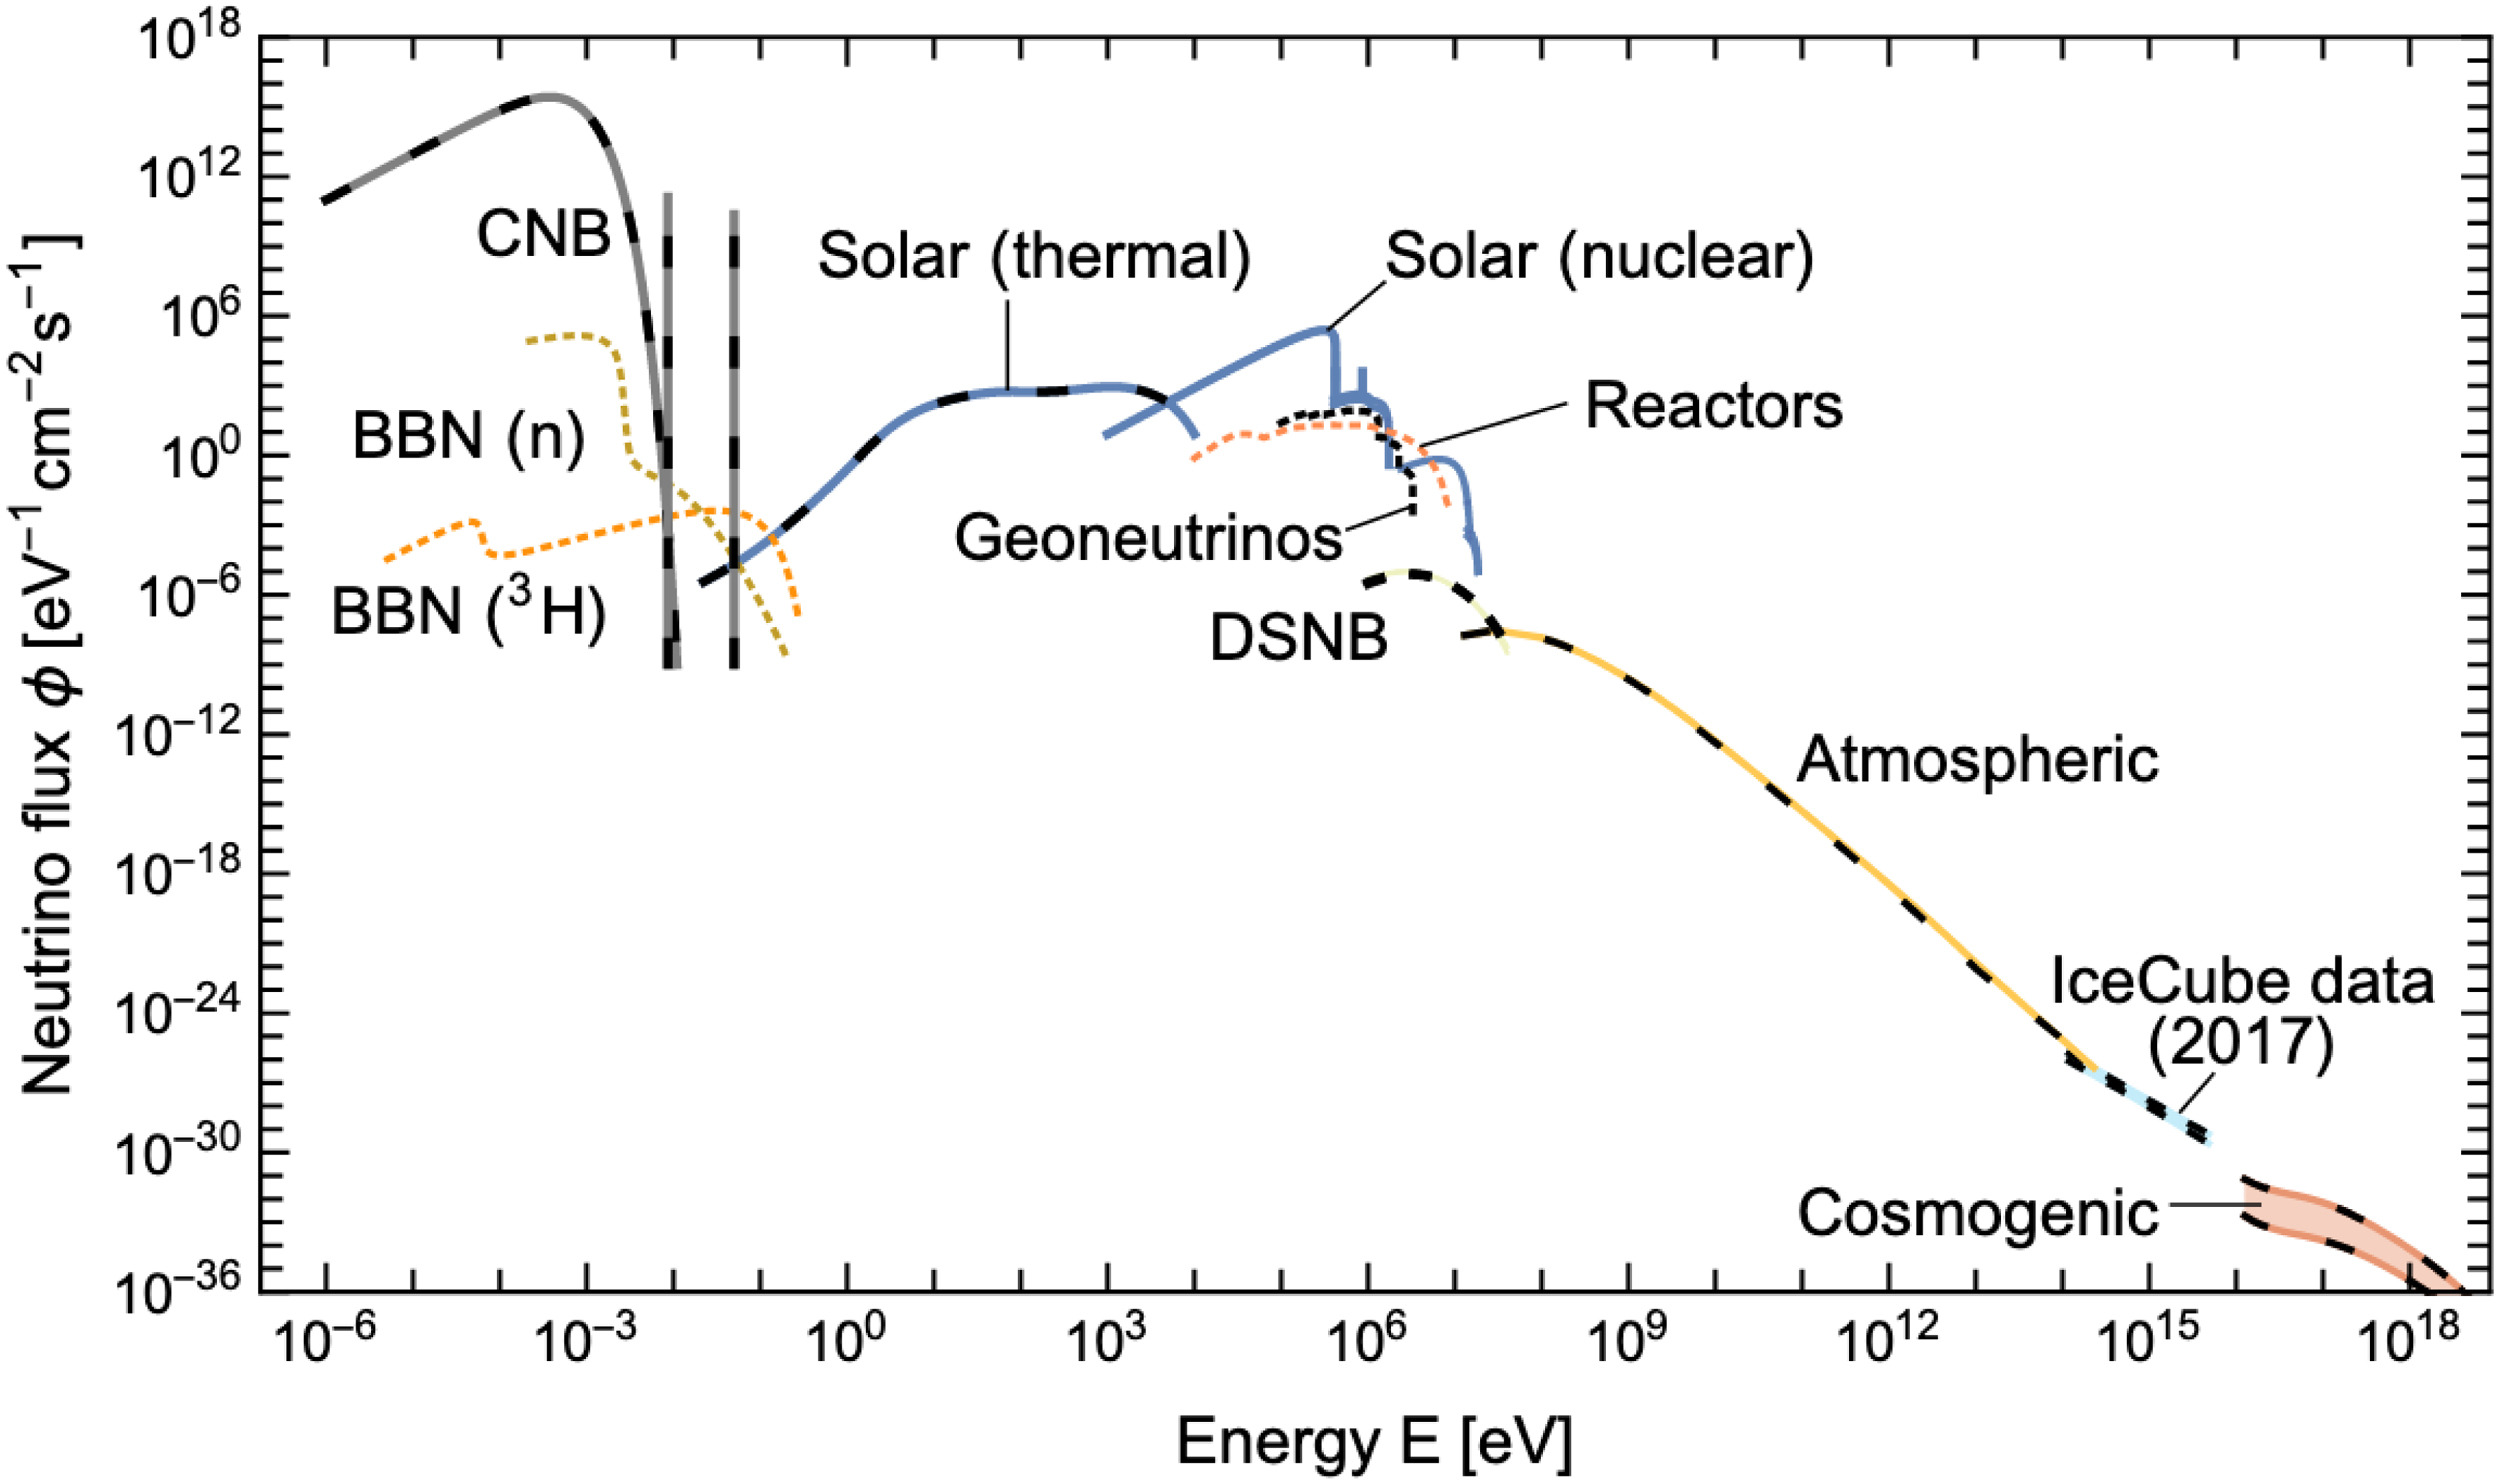
\includegraphics[width=14.5cm]{thesis_figures/CRnNu/Neutrino spectra.jpg}
  \caption{Grand Unified neutrino spectra at Earth. Taken from~\cite{Vitagliano:2019yzm}}.
  \label{fig:Neutrino-spectra}
\end{figure}

Neutrinos arriving at Earth through astrophysical sources such as the Sun have also played an important role in increasing our understanding of \glspl{CR} and physics in general. The solar neutrino observations ultimately led to the postulation and discovery of neutrino oscillations. The observations of neutrinos from SN 1987A, a type II supernova in the Large Magellanic Cloud by Kamiokande II~\cite{PhysRevLett.58.1490} before the observation of any other messenger marked the dawn of non-solar neutrino astronomy and displayed the importance of neutrinos for multi-messenger physics. One of the most important experiments in this field has been the IceCube Observatory. Located at the South Pole it has revolutionized both neutrino and multi-messenger astronomy. It has led to the first detection of astrophysical neutrinos~\cite{PhysRevLett.111.021103} and provided a measurement of their spectrum for high energies~\cite{doi:10.1126/science.1242856}. It has also contributed to the study of the neutrino oscillations~\cite{Abbasi_2023_Oscillation} and could also help with $\nu$ mass hierarchy~\cite{psf2023008007}. Recently, IceCube has further found indications for the first source of steady-state neutrinos in our cosmos which is the NGC1068~\cite{Icecube_2022} and has also led to the groundbreaking measurement of the neutrino spectrum from our Galaxy~\cite{Galactic_plane_nu_2023}. These results and their implications are discussed in more detail in section~\ref{subsec:Nuresults}. Its contributions to multi-messenger astronomy are also discussed later in section~\ref{sec:Mul-mes}. For the highest of energies, the Pierre Auger Observatory remains the only facility capable of detecting neutrinos. 
Neutrinos can help to understand various astrophysical processes such as the Big Bang where the neutrinos are hypothesized to have decoupled one second after leading to \gls{CNB}~\cite{scott2024cosmicneutrinobackground} to the nuclear processes inside stellar objects. Each such process speculates a unique neutrino spectrum which can be probed with experiments to garner their viability. Figure~\ref{fig:Neutrino-spectra} shows the unified neutrino spectrum (measure and expected) with respect to energy. For this thesis, the following sections are constrained to only the neutrinos of the highest energies (\glspl{UHEnu}) above $10^{16}$ eV. How neutrinos can help decipher the mysteries of \glspl{UHECR} is also discussed below.

\subsection{Origin and Propagation}
\label{subsec:nuorig}
UHE$\nu$s can be broadly classified into three categories based on their origin. These are astrophysical, originating from known/hypothesized astrophysical sources, cosmogenic, originating from the interactions of \glspl{UHECR} with the \gls{CMB} or the \gls{EBL} and exotic, emerging from processes such as the Big Bang, dark matter annihilation etc. The reactions for the mentioned processes are as follows:
\subsubsection*{Astrophysical Neutrinos}
\label{subsubsec:AstroNu}

Astrophysical neutrinos are thought to be produced by or around known sources of \glspl{UHECR}. The most important ingredients that are required to produce UHE$\nu$s are the interactions of high-energy protons and nuclei with matter or radiation fields which result in photo-meson production followed by a charged pion decay. The decay length of pions is much shorter than the distances of the sources to Earth thus they decay and give rise to secondary neutrinos. 

\begin{subequations}\label{eq:Nuprod_1}
  \begin{align}
    \begin{split}
      p + \gamma &\longrightarrow \Delta^+(1232 ) \longrightarrow n+\pi^+ \\ 
                      &\longrightarrow \Delta^+(1232 ) \longrightarrow p+\pi^0
    \end{split} \\
      p + \bar{p} &\longrightarrow \pi^- + \pi^+ + \pi^0 
  \end{align}
\end{subequations}

\begin{subequations}\label{eq:Nuprod_2}
  \begin{align}  
    \pi^0 &\longrightarrow \gamma + \gamma \\
    \pi^+ &\longrightarrow \mu^+ + \nu_{\mu} \longrightarrow e^+ + \nu_{e} + \bar{\nu}_{\mu} + \nu_{\mu} \\
    \pi^- &\longrightarrow \mu^- + \bar{\nu}_{\mu} \longrightarrow e^- + \bar{\nu}_{e} + \nu_{\mu} + \bar{\nu}_{\mu}
  \end{align}
\end{subequations}

Other interactions such as beta decay of neutrons and nuclei ($n \longrightarrow p + e^- + \bar{\nu}_{e} $, \\$(A, Z) \longrightarrow (A, Z-1/ Z+1) + e^{+/-} + \nu_{e} / \bar{\nu}_{e}$), electron/positron capture and $\beta$ decays can also contribute to neutrino production. In most of these scenarios the expected flux ratio per flavor can be either $ \nu_{e} : \nu_{\mu} : \nu_{\tau} = \bar{\nu_{e}}: \bar{\nu_{\mu}}: \bar{\nu_{\tau}} = (1:2:0) $ or (1:0:0) with no direct known process for $\nu_{\tau}$ production at the source. However, since neutrinos can oscillate which is a consequence of the mixing between the flavor  $\left| \nu_{\alpha} \right\rangle $ and mass eigenstates $\left| \nu_{i} \right\rangle $  of neutrinos, given by the following relation:
\begin{equation}
\left| \nu_{\alpha} \right\rangle  = \sum_i U_{\alpha i} \left| \nu_{i} \right\rangle,
\end{equation}
\begin{figure}[t!]
  \centering
  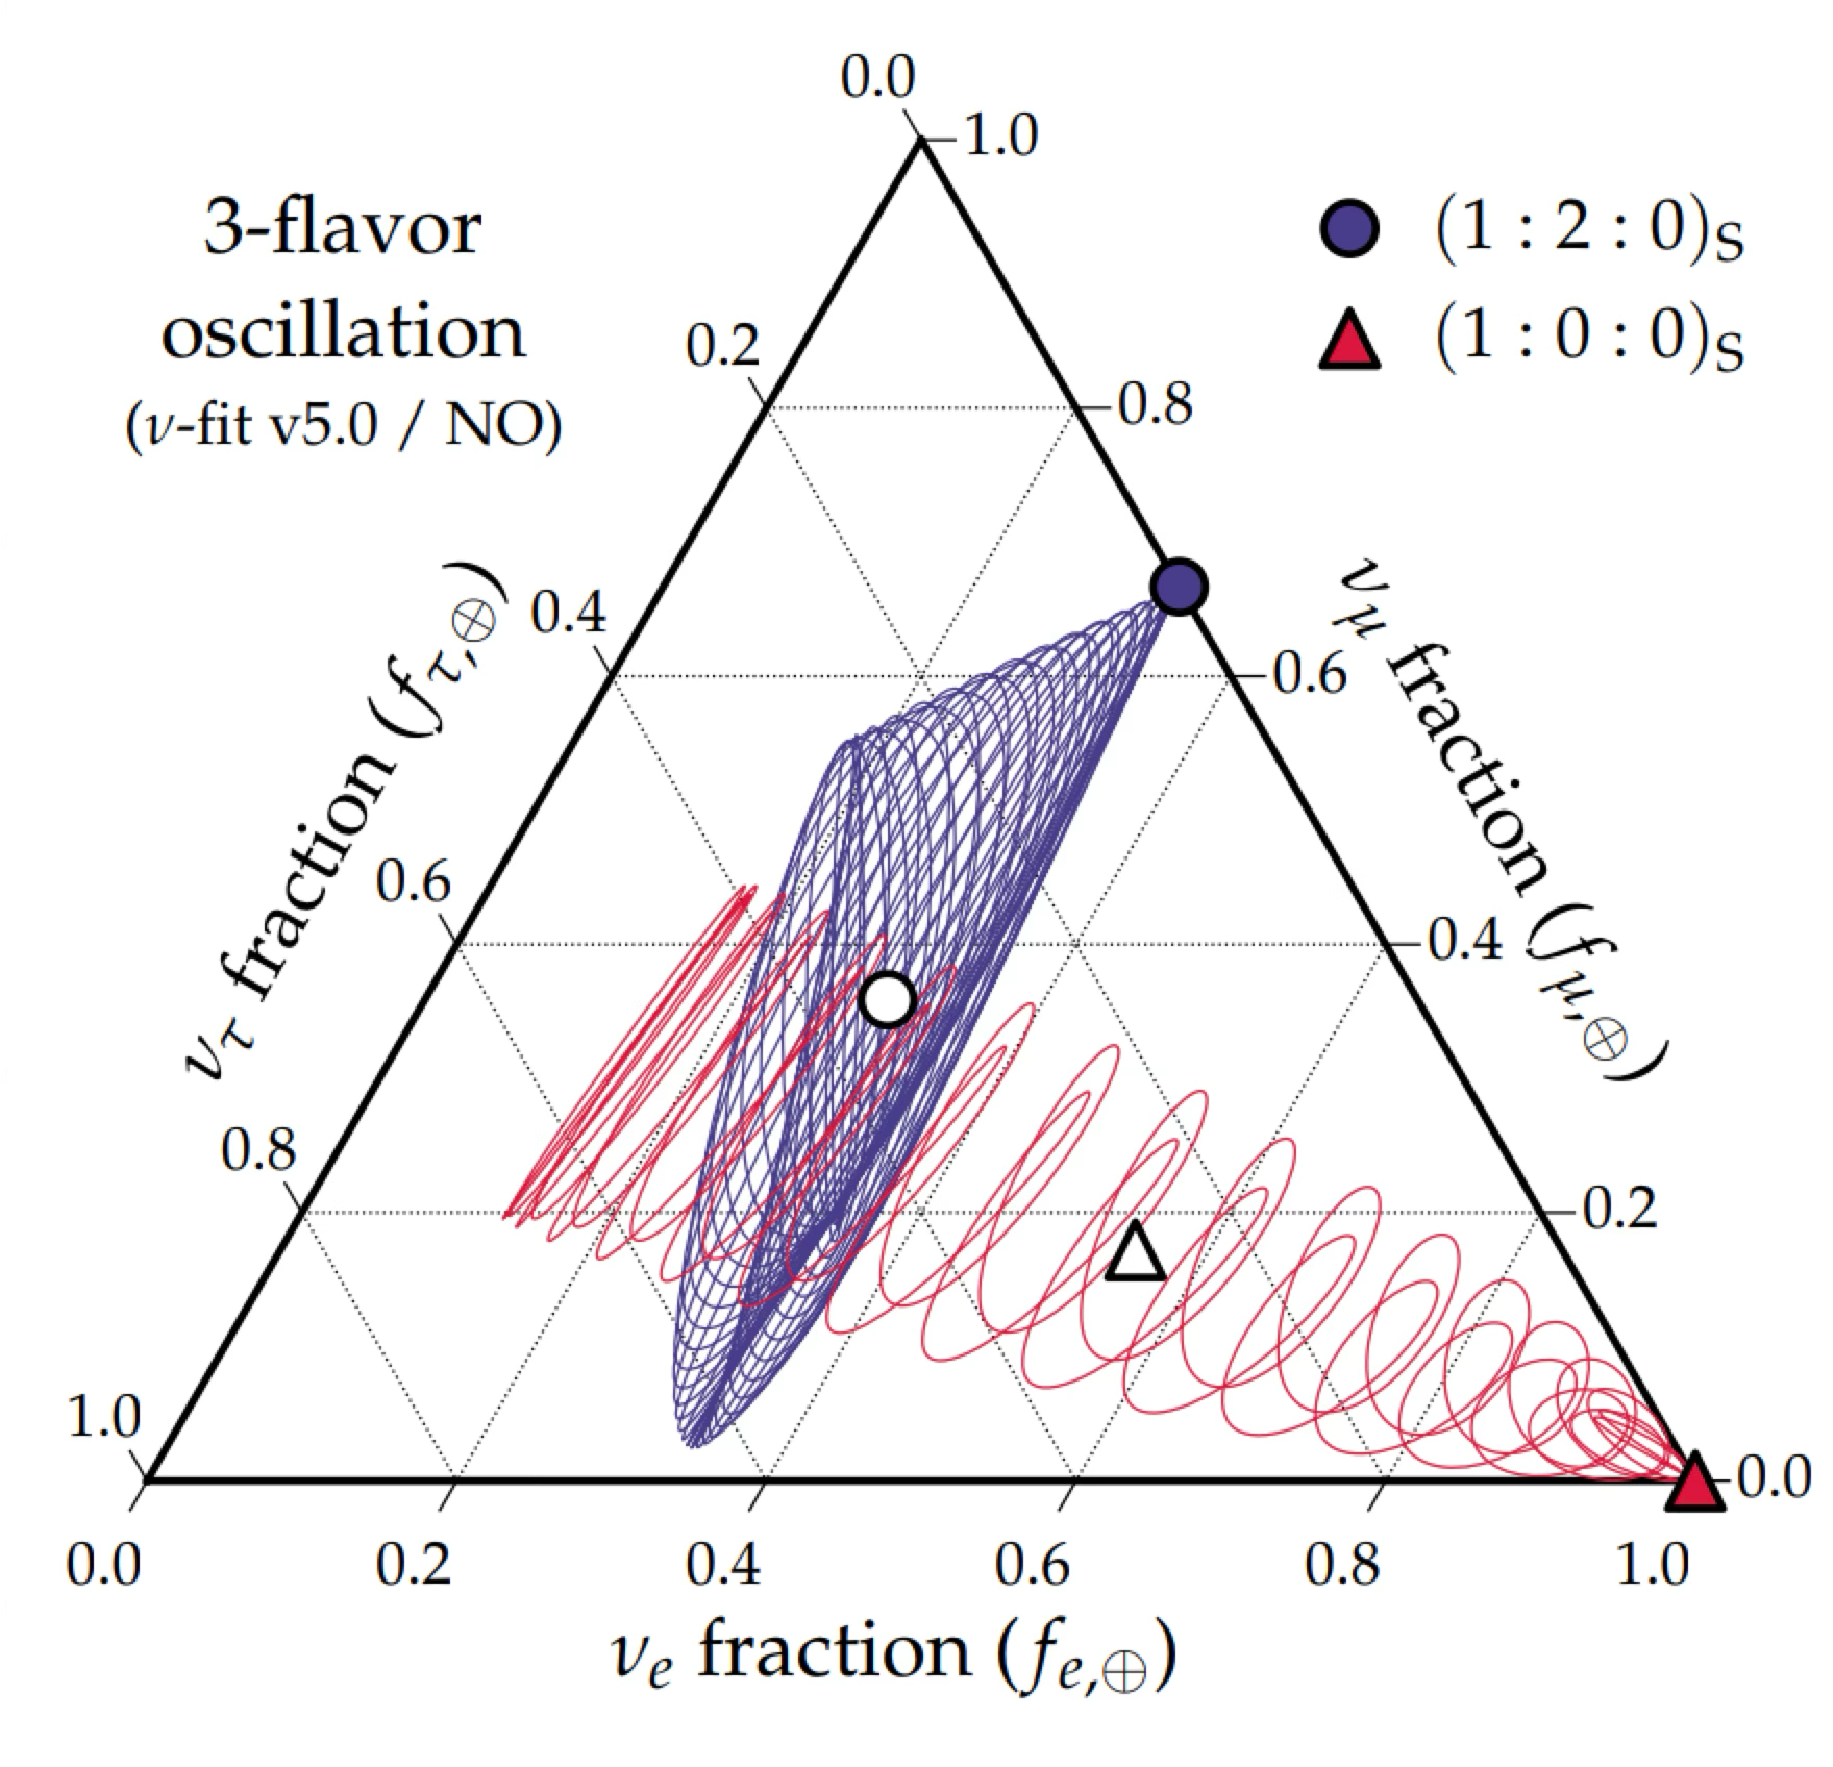
\includegraphics[width=12.5cm]{thesis_figures/CRnNu/Oscillation_sim_ternary.pdf}
  \caption{A ternary plot to show the neutrino flavor oscillations. Two different flux ratios per flavor (circle, triangle) based on different production mechanisms are shown. Flavors expected after propagation are also marked (open shapes). Taken from~\cite{Ahlers:ISAPP2022}}.
  \label{fig:Oscillation_ternary}
\end{figure}

where $U_{\alpha i}$ is the mixing matrix formulated by Pontecorvo-Maki-Nakagawa-Sakata~\cite{Pontecorvo:1957qd,10.1143/PTP.28.870}. In a standard case where three neutrino flavors are considered this matrix is a 3x3 matrix parameterized by the three mixing angles ($\theta_{12},\theta_{23},\theta_{13}$) and a single phase called $\delta_{\text{CP}}$. Starting from the expected source flavor ratio one can calculate the flavor ratio at Earth by knowing the above four mentioned parameters. One example of such propagation is shown in Fig.~\ref{fig:Oscillation_ternary}. Since high energy tau neutrinos are not expected to be present in the atmospheric neutrino background the detection of such neutrinos at Earth could be an indication that the neutrino had an astrophysical origin. 

Another important aspect to fully understand the origin and propagation of astrophysical neutrinos is determining their expected energies. On average the energy fraction that pions can get from the \gls*{CR} nucleons is about 20\%. These relativistic pions can then further pass on between $\sim$20-26\% depending on the flavor and type of the neutrino. Approximately, the energy fraction for the produced neutrinos concerning the gamma and nucleon is~\cite{Lipari_2007}:
\begin{equation}
  \left\langle E_{\nu} \right\rangle  \simeq  \frac{1}{2}\left\langle E_{\gamma} \right\rangle \simeq  \frac{1}{20}\left\langle E_{N} \right\rangle
\end{equation}
Depending on the type of source and how far the said source is one can calculate the maximum energy potential for sources. With the measurement of the diffused astrophysical flux~\cite{PhysRevD.110.022001} by IceCube up to $10^{16}$eV, these calculations can be directly constrained by measurement~\cite{Abbasi_2023_supernova_emission}. Since extragalactic sources can produce \glspl{UHECR} up to $\sim 10^{20}$eV which is corroborated by measurements of the Pierre Auger Observatory one can calculate an upper limit to the diffuse flux for neutrinos from some hypothesized sources such as Starburst galaxies~\cite{Condorelli_2023_starburst}, AGNs~\cite{Murase_2023} and Magnetars~\cite{2003ApJ...595..346Z}. The non-detection of UHE$\nu$s at Auger can thus also act as an important tool to constrain the production mechanisms hypothesized for these sources. The potential of this is discussed later in section~\ref{subsec:Nuresults}.   

\subsubsection*{Cosmogenic Neutrinos}
\label{subsubsec:CosmoNu}

\begin{figure}[t!]
  \centering
  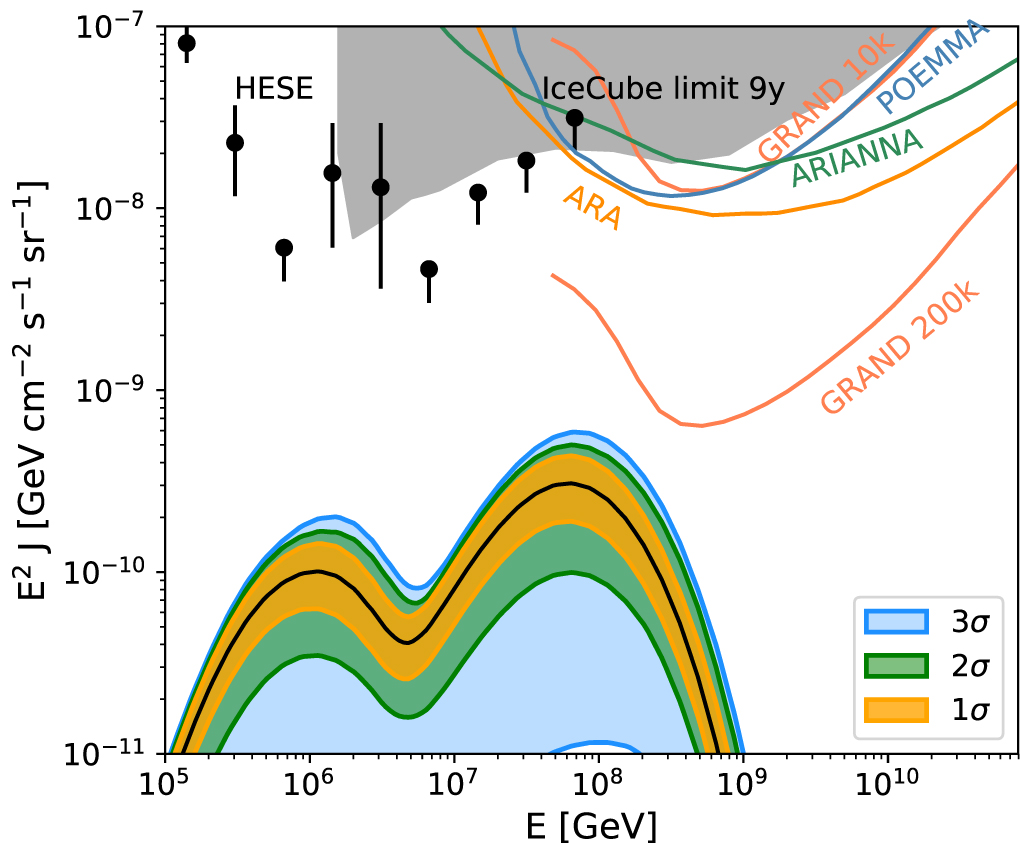
\includegraphics[width=14.5cm]{thesis_figures/CRnNu/apjab05cef9_hr.jpg}
  \caption{Allowed confidence ranges for cosmogenic neutrino fluxes obtained by varying the parameters regarding the source distribution and emission. The figure illustrates the two mechanisms of production of with the first peak corresponding to neutrinos from neutron decay and the peak at 10$^{18}$eV corresponds to neutrinos from meson decay. Taken from~\cite{Heinze:2019jou}}
  \label{fig:model_nu_auger_mixed}.
\end{figure}

Cosmogenic neutrinos are produced either as a consequence of the \gls{GZK} mechanism discussed in section~\ref{subsubsec:GZK} or due to the interactions of \glspl{UHECR} with \gls{EBL}. They were first suggested by Berezinsky and Zatsepin in 1969~\cite{Berezinsky:1970xj}. The processes involved are similar to those for astrophysical neutrinos albeit the proton/nuclei interact with the CMB/EBL photon instead of the photons from the radiation fields. The two main processes are the same as that for the GZK mechanism i.e. decay of charged pions produced in photo-pion production, eq.~\ref{eq:GZK} and the beta decay of neutrons and nuclei produced in photo-disintegration, eq.~\ref{eq:Pdisinteg}. \gls{CMB} mainly affects the protons~\cite{Ehlert_2024} during their propagation which form a large fraction of the \glspl{UHECR} traversing the universe while the EBL plays an important role in the case of other nuclei~\cite{Aloisio_2015}. 
Since the processes are the same, the flavor flux expectations at Earth remain the same. However, the expected energies that the cosmogenic neutrinos can acquire differ drastically as compared to astrophysical neutrinos. The energy of neutrinos produced due to interactions with \gls*{CMB} in the case of photo-pion production is of the order of $10^{18}$eV while for the ones produced via the by-products (pions or neutrons) of photo-disintegration, it is of the order of $10^{16}$eV~\cite{Aloisio_2015}. In the case of interactions with \gls*{EBL}, this lowers to about $10^{15}$eV and $10^{14}$eV for the two types of interactions. 
The exact properties of the neutrinos produced are directly dependent on the parent \glspl*{UHECR} that produce them. The properties of \glspl{UHECR} such as the total flux, composition, maximum energies, production spectrum at the sources and their cosmological evolution (adiabatic losses) are all crucial factors that affect the  secondary cosmogenic neutrinos produced by these \glspl*{UHECR}. A collection of some examples of the expected cosmogenic neutrino fluxes for different scenarios can be found in ~\cite{KAMPERT2012660,AlvesBatista:2018zui,Heinze:2019jou}. One example are shown in Fig.~\ref{fig:model_nu_auger_mixed}. The two distinct humps are due to the two associated production processes with the lower one being due to the neutrinos produced in beta decay of neutrons and the higher one caused by nuclei produced via photo-disintegration. 

Measurements of \gls*{CR} detection observatories such as the Pierre Auger Observatory can also be used to calculate an expected neutrino spectrum based on assumptions on the composition and the cosmological evolution of the sources. Neutrinos thus can act as a very important tool in constraining the composition of the incoming \glspl*{UHECR} and furthering their actual sources. They can also help to solve the question of the cutoff observed in the \gls*{UHECR} spectrum whether this is due to the \gls*{GZK} mechanism (proton-dominated composition) or sources reaching their maximum potential as theorized by Hillas (mixed composition). The current results regarding this important study are discussed in section~\ref{subsec:Nuresults}.
\subsubsection*{Exotic Neutrinos}
\label{subsubsec:ExoticNu}
Neutrinos can also be produced as a result of self-annihilation or decay of dark matter particles. In dark matter annihilation scenarios, two dark matter particles come together and annihilate, leading to the production of standard model particles as a result. The specific flux of the neutrino depends on the properties of the dark matter particle. One such candidate for such a process could be a \gls{WIMP}, which could be its own antiparticle (a Majorana fermion). In regions with a high concentration of dark matter, such as the centres of galaxies or galaxy clusters, \glspl{WIMP} can come together and annihilate into standard model particles~\cite{10.1111/j.1365-2966.2008.13366.x}. One of the annihilation channels of interest for producing very high-energy neutrinos is the annihilation into pairs of intermediate bosons, such as $W^+W^-$ (W-boson pair), or $Z^0 - Z^0$ (Z-boson pair). These intermediate bosons can subsequently decay into quarks, leptons, and other particles, including neutrinos. The final state neutrinos can be very high-energy, potentially reaching energies in the peta-electronvolt (PeV) range and beyond. For dark matter decay, a stable dark matter particle is supposed to spontaneously transform to other standard model particles including neutrinos~\cite{PhysRevD.108.123021}. 

\subsection{Neutrino Interactions and Detection}
\label{subsec:Nuintdet}

The low interaction cross-section ($\sigma_{\nu}$)~\cite{Formaggio_2012} of neutrinos which allows them to travel for large distances also makes them almost impossible to detect. They can pass through vast amounts of material without leaving a significant trace. While at low energies processes such as Inverse Beta Decay are used to detect the neutrinos, at high energies neutrinos can interact via \gls{CC} and \gls{NC} Interactions. In \gls*{CC} interaction, a neutrino interacts with a target nucleus with an exchange of a W boson, transforming into a charged lepton corresponding to the flavor of the incoming neutrino and a hadronic cascade. The NC interaction is flavor blind and occurs with an exchange of the $Z^0$ boson and a nuclear recoil. Both reactions are shown in the equations below:

\begin{subequations}\label{eq:NuCC_NC}
  \begin{align}
    \begin{split}
      \nu_l \, (\bar{\nu_l}) + N &\mathop{\longrightarrow}^{\mathrm{CC}} l^- \, (l^+) + X 
    \end{split} \\
    \nu_l \, (\bar{\nu_l}) + N &\mathop{\longrightarrow}^{\mathrm{NC}} \nu_l \, (\bar{\nu_l}) + X
  \end{align}
\end{subequations}

The products from the CC and NC interaction i.e. a lepton and the hadronic cascade can be detected in multiple ways. 
Antineutrinos can also interact with atomic electrons leading to a $W^-$ boson production called the Glashow resonance~\cite{PhysRev.118.316}. The threshold antineutrino energy for such a reaction to occur is $\sim$6.3 PeV. This process dominates the CC and NC interaction albeit only in a small energy range. Proposed in 1959, it was first observed at the IceCube Observatory~\cite{IceCube:2021rpz}. Both CC and NC when interacting with the nucleon undergo neutrino-nucleon deep inelastic scattering where the interacting neutrino scatters off individual quarks inside nucleons (protons or neutrons), leading to the fragmentation of the nucleon and the creation of hadronic (particles made of quarks) jet. At low center-of-mass energies ($\sim$TeV) accelerators can provide most of the information about the neutrino interaction with matter and the corresponding cross-section but at high energies this estimation can either only be calculated via the detection of astrophysical and cosmogenic neutrinos or via a robust theoretical estimation including \gls{QCD} and low energy measurements. The description of \gls*{QCD} at such high energies is still not completely understood. Moreover, physics beyond the Standard Model can also be introduced for these energies which can further affect the neutrino cross-section estimation~\cite{PhysRevD.107.033009}. For the purpose of this thesis, the neutrino cross-sections calculated in~\cite{Cooper_Sarkar_2011} are used. The reference provides an updated $\nu -N$ cross-section calculations with corresponding uncertainties, taking into account the full HERA~\cite{aaron2010combined} data release and combining it with the DGLAP~\cite{ALTARELLI1977298,Dokshitzer:1977sg,Gribov:427157} formalism of QCD. Based on the expected flux the cross-section and the energy of neutrinos it is easy to calculate minimum detector sizes for high-energy neutrinos. For example, for a neutrino of energy $E_{\nu} \sim 1\,\text{PeV} = 10^{15}\,\text{eV}$, the expected flux is $\frac{d^2N_{\nu}}{dt dA} \sim \frac{1}{cm^2 \times 10^5 yr}$, the cross-section is $\sigma_{\nu N} \sim 10^{-8} , \sigma_{pp} \sim 10^{-33}$ and the targets can be estimated as $ N_N \sim N_A \times V/cm^3$ where $N_A$ is the Avogadro's number then the rate of expected events is given by:

\begin{equation}
  N_{\nu} \sim N_N \times \sigma_{\nu N} \times \frac{d^2N_{\nu}}{dt dA} \sim \frac{1}{\text{yr}} \times \frac{V}{1\,\mathrm{km^3}}
\end{equation}

Therefore, to detect a neutrino at this energy range in a year requires a detector with a minimum size of 1km$^3$. The type of such large volume detectors for UHE$\nu$s depends on the particular techniques used to detect the products of neutrino interaction with nucleon. 

The charged lepton can produce detectable signals via ionization, Cherenkov radiation or scintillation. Moreover, the lepton and hadrons can also trigger EASs which can be detected. Both the lepton and the hadron can lead to a cascade. Depending on the flavor of the neutrino the interaction also leads to unique signals. The electron produced in the CC interaction of $\nu_e$ produces electromagnetic cascades in the propagation medium while a muon rarely produces a cascade like signature only undergoing radiation losses. In contrast, a tau lepton produced from $\nu_{\tau}$ can propagate without interaction for a certain distance and then lead to a cascade. For NC reactions the leptonic cascade is missing and only a hadronic cascade can be observed. Low-energy neutrinos or neutrinos produced in the atmosphere can also lead to similar cascades and act as background for high-energy neutrino searches. Depending on the location and techniques employed such background is dealt with in different ways. Some examples of different detectors based on the medium and the methodology employed for detection are as follows:

\begin{figure}[t!]
  \centering
  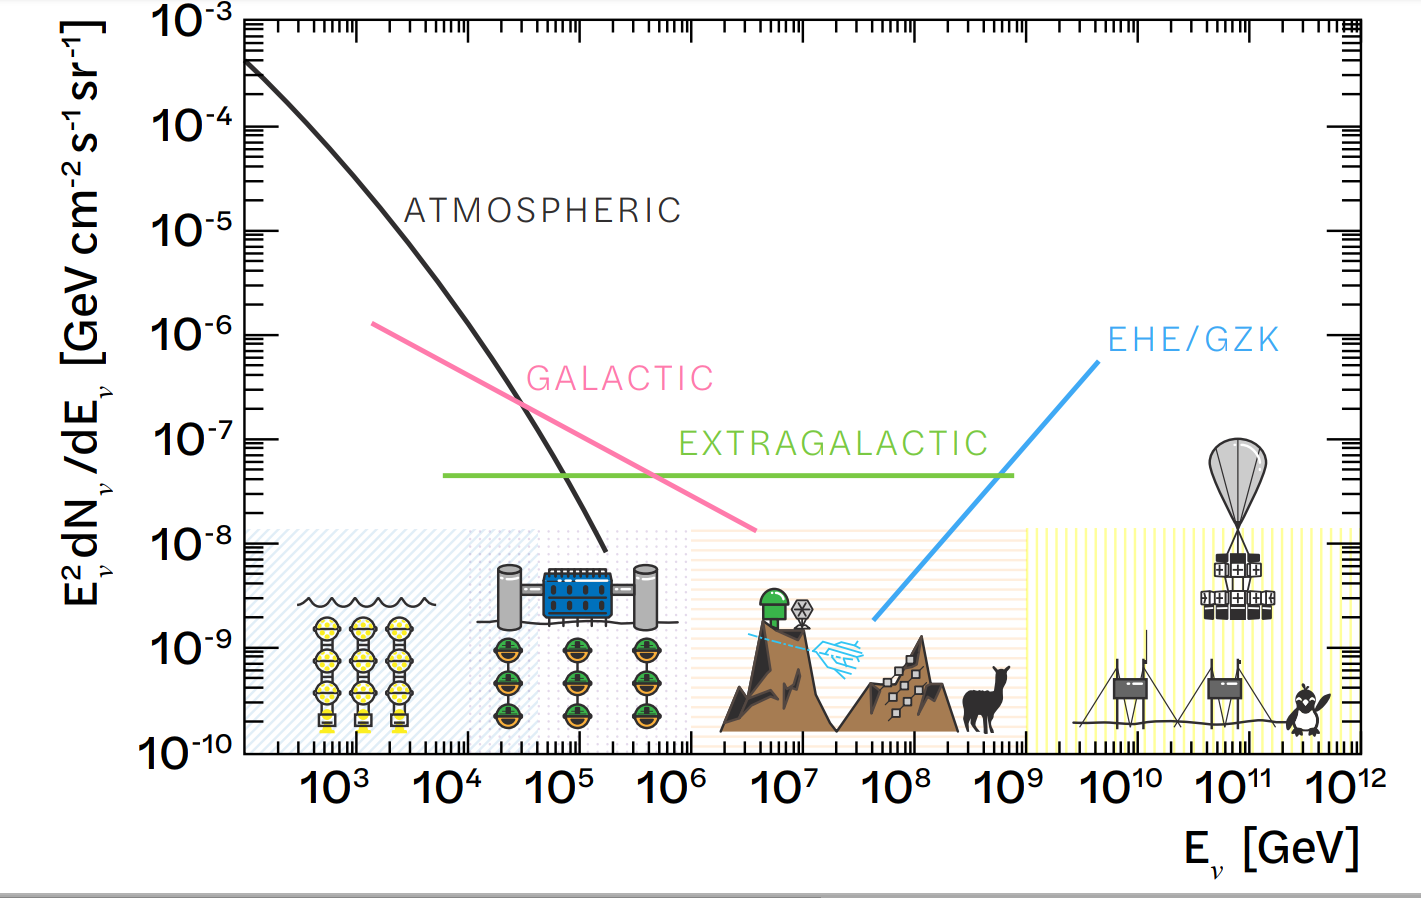
\includegraphics[width=14.5cm]{thesis_figures/CRnNu/UHE_nu_techniques.png}
  \caption{Different detection techniques for UHE neutrinos. Ice and Water based Cherenkov detectors are sensitive to atmospheric, galactic neutrinos and some extragalactic neutrinos while radio and air shower detectors are sensitive to very high energy neutrinos with other techniques filling the gaps. The spectral indices of the different components are estimations. Taken from~\cite{Arguelles:2024xkx}}.
  \label{fig:UHE-nu-techniques}
\end{figure}

\begin{description}
  \item \textbf{Ice and Water Cherenkov Detectors:} IceCube Neutrino Observatory~\cite{Aartsen_2017} and its predecessor AMANDA~\cite{WISCHNEWSKI1999412} are examples of in ice Cherenkov detectors. IceCube is located at the South Pole and uses a cubic-kilometer array of Antarctic ice to detect high-energy neutrinos. It consists of 80 strings carrying 60 photomultiplier detectors each situated between 1500 m and 2500\,m below the surface. Neutrinos interact with the optically clear ice nuclei, producing secondary particles that emit Cherenkov radiation. The detector's photomultiplier tubes capture the Cherenkov light, allowing reconstruction of the neutrino direction and energy. Muon tracks resulting from CC interactions can also be observed. Being underground partly shields IceCube from the atmospheric neutrino background which is useful for down-going neutrinos. It can also use the Earth as a shield to look for PeV upward-going neutrinos. The Observatory also consists of a surface array (IceTop) of ice Cherenkov tanks which further help in atmospheric background rejection and CR studies. 
  
  Water based Cherenkov detectors have been used for neutrino detection since their discovery. Kamiokande II~\cite{Arisaka:1984aoa} used a large underground water tank surrounded by PMTs to observe the first astrophysical neutrinos from SN 1987A~\cite{PhysRevLett.58.1490}. Since the required detector volume for detection of a sufficient rate of neutrinos is very large, sizeable stable natural water reservoirs are used to build such detectors. Some examples include the ANTARES~\cite{CREUSOT2013489} and KM3Net~\cite{MARGIOTTA201483} located in the Mediterranean Sea off the coast of France and Italy and the upcoming BAIKAL-GVD~\cite{MALYSHKIN2023168117} and P-ONE~\cite{P-ONE:2020ljt} located in Lake Baikal, Russia and the Pacific Ocean off the coast of British Columbia, Canada respectively. The actual detector and the principle remain the same as IceCube with the only change being the medium and upgrades in detector technology depending on the advances in the field. 
  
  \item $-$ \textbf{Radio Detectors:} These detectors are based on the detection of $\nu$s in dense media using the Askaryan effect~\cite{Askaryan:1961pfb,PhysRevD.84.103003}. It is a phenomenon in which high-energy charged particles moving through a dense dielectric medium, produce coherent electromagnetic radiation in the radio frequency range.  When the high-energy particles interact with the atoms and molecules in the dielectric medium, they generate a shower of secondary charged particles. As these secondary particles move through the medium they undergo a charge separation leading to the emission of coherent Cherenkov radiation in the radio frequency range. The effect typically produces radiation in the radio frequency range, from a few hundred \gls{MHz} to several \gls{GHz}. Experiments like ANITA~\cite{ANITA:2008mzi} have tried to detect the radio emission produced when neutrinos interact with the Antarctic ice~\cite{Schoorlemmer_2016}. RNO-G ~\cite{Aguilar_2021}, an in ice radio antenna array, is also under construction at Summit Station in Greenland to search for neutrinos above PeV energies. The planned upgrade of IceCube, IceCube-Gen-2~\cite{Aartsen_2021_Gen-2} also plans to employ a large in ice radio array to increase its sensitivity to both astrophysical and cosmogenic neutrinos. 
  
  \item $-$ \textbf{Acoustic Detectors:}  The cascade of secondary particles produced in a neutrino interaction in a medium can also generate an acoustic shockwave, also known as a "thermoacoustic pulse," due to rapid heating and expansion of the medium. The resulting acoustic signal travels through the medium as a pressure wave and can be detected by sensitive acoustic sensors. Typically, large volumes of water or ice are used as the detection medium. The acoustic signal propagates through the medium and can be detected by underwater microphones (hydrophones) or other acoustic detectors. This technique has not yet yielded a neutrino observation. It has been used at ANTARES as AMADEUS~\cite{LAHMANN2012S216} and at IceCube as SPATS~\cite{Karg_2012} to test the acoustic properties. ANDIAMO~\cite{Marinelli_2022} is a proposed acoustic neutrino detector that could use this technique in the future.
  
  \item $-$ \textbf{Radar Echo Detectors:} Radar Echo Telescope~\cite{Prohira_2021} is a detector that aims to detect neutrinos using the radar echo method. The method is based on the reflection of a transmitted radar signal by the in ice neutrino cascade which acts as a short-lived mirror. The reflected signal is then detected at a receiving antenna. This technique is currently being tested in Greenland for Cosmic ray showers and might be employed to detect neutrinos in the future.

  \item $-$ \textbf{Air Shower Detectors:} Even though, the typical interaction lengths of UHE$\nu$s are way larger than the atmospheric depth, neutrinos can still induce an EAS. Such EASs can develop at any point in the atmosphere, due to the virtually constant neutrino cross-section in air, in comparison to \glspl{CR} offering a distinctive aspect for detection at \gls{CR} observatories like the Pierre Auger Observatory. Pierre Auger Observatory uses the said property to search for EeV neutrinos. EASs and the expected signature at the Pierre Auger Observatory for both \glspl{CR} and neutrinos are discussed in the next Chapter~\ref{chap:EAS}.   

  \end{description}

\subsection{Latest results}
  \label{subsec:Nuresults}
  
\subsubsection*{Astrophysical Neutrinos}

\begin{figure}[t!]
  \centering
  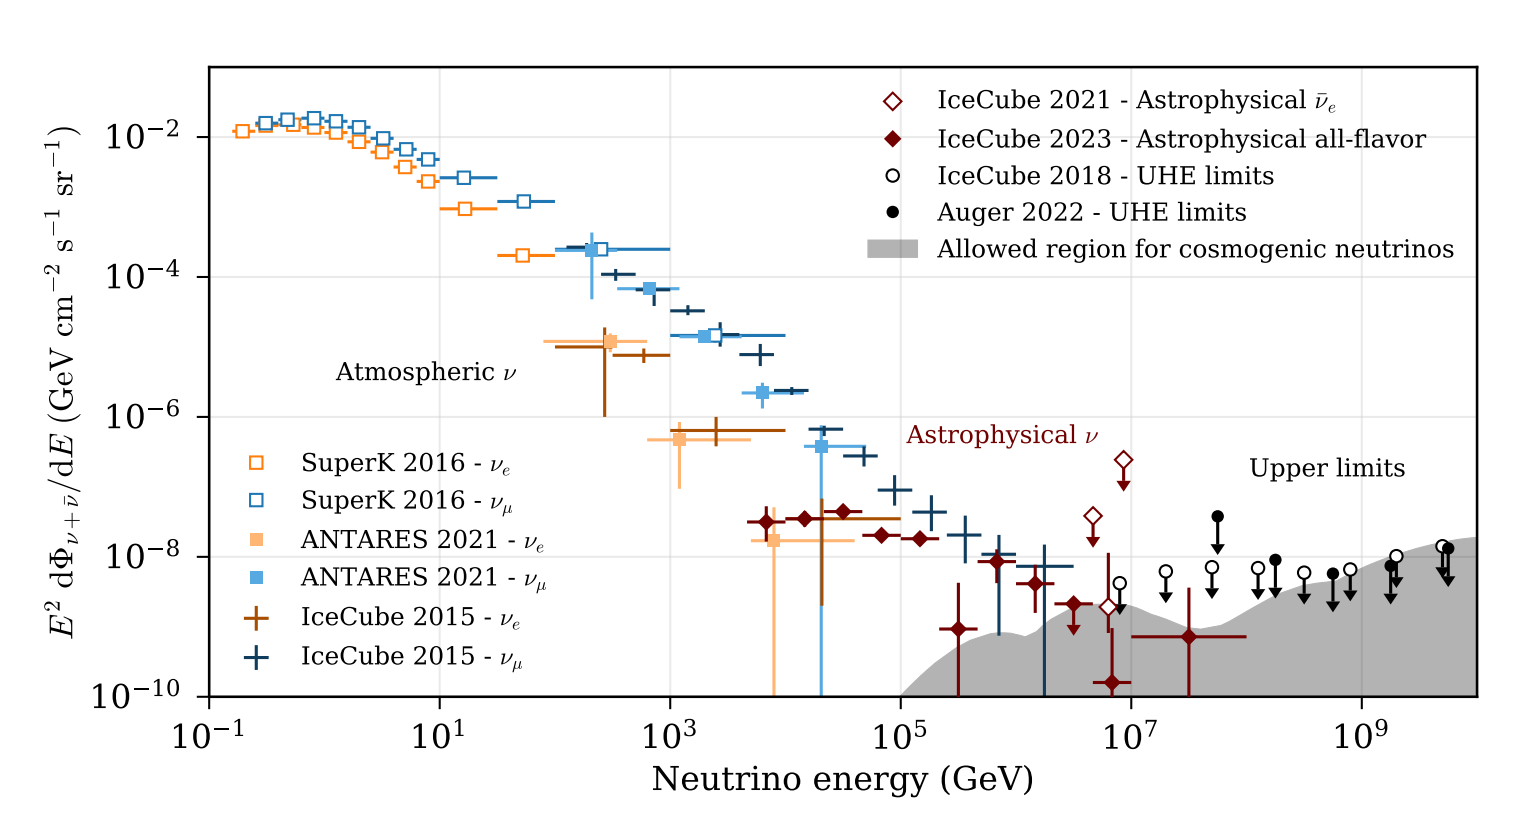
\includegraphics[width=14.5cm]{thesis_figures/CRnNu/Nu_flux_measurement.png}
  \caption{Measured neutrino flux for atmospheric and astrophysical neutrinos. At high energies for the diffuse flux of cosmogenic neutrinos there are upper limits from IceCube and the Pierre Auger Observatory. Taken from~\cite{ParticleDataGroup:2024cfk}}.
  \label{fig:Nu_flux_measurement}
\end{figure}

  \paragraph*{Spectrum}
  \label{subsubsec:Nuspectrum}
  After the measurements of astrophysical neutrinos at the IceCube Neutrino Observatory, the first plot and estimation of flux has been possible for high-energy neutrinos. The flux spectrum as measured by IceCube and other experiments is shown in Fig.~\ref{fig:Nu_flux_measurement}. The flux was first published in 2013~\cite{Aartsen_2014_first_flux} and has since been refined with various analyses~\cite{PhysRevD.110.022001}. The plot also shows the summary of the currently published analysis along with current best upper limits for cosmogenic neutrino flux. The diffuse flux spectrum agrees across the various analyses within the overlapping energy regions. However, there is a slight tension between the estimate of the spectral index which is obtained after fitting the flux spectrum. The measurements are also not enough to decide on the nature of the flux across the whole energy range and more measurements in the future would help understand the neutrino spectrum in more detail. 

  \paragraph*{Sources}
  \label{subsubsec:Nusources}
  \begin{figure}[t!]
    \centering
    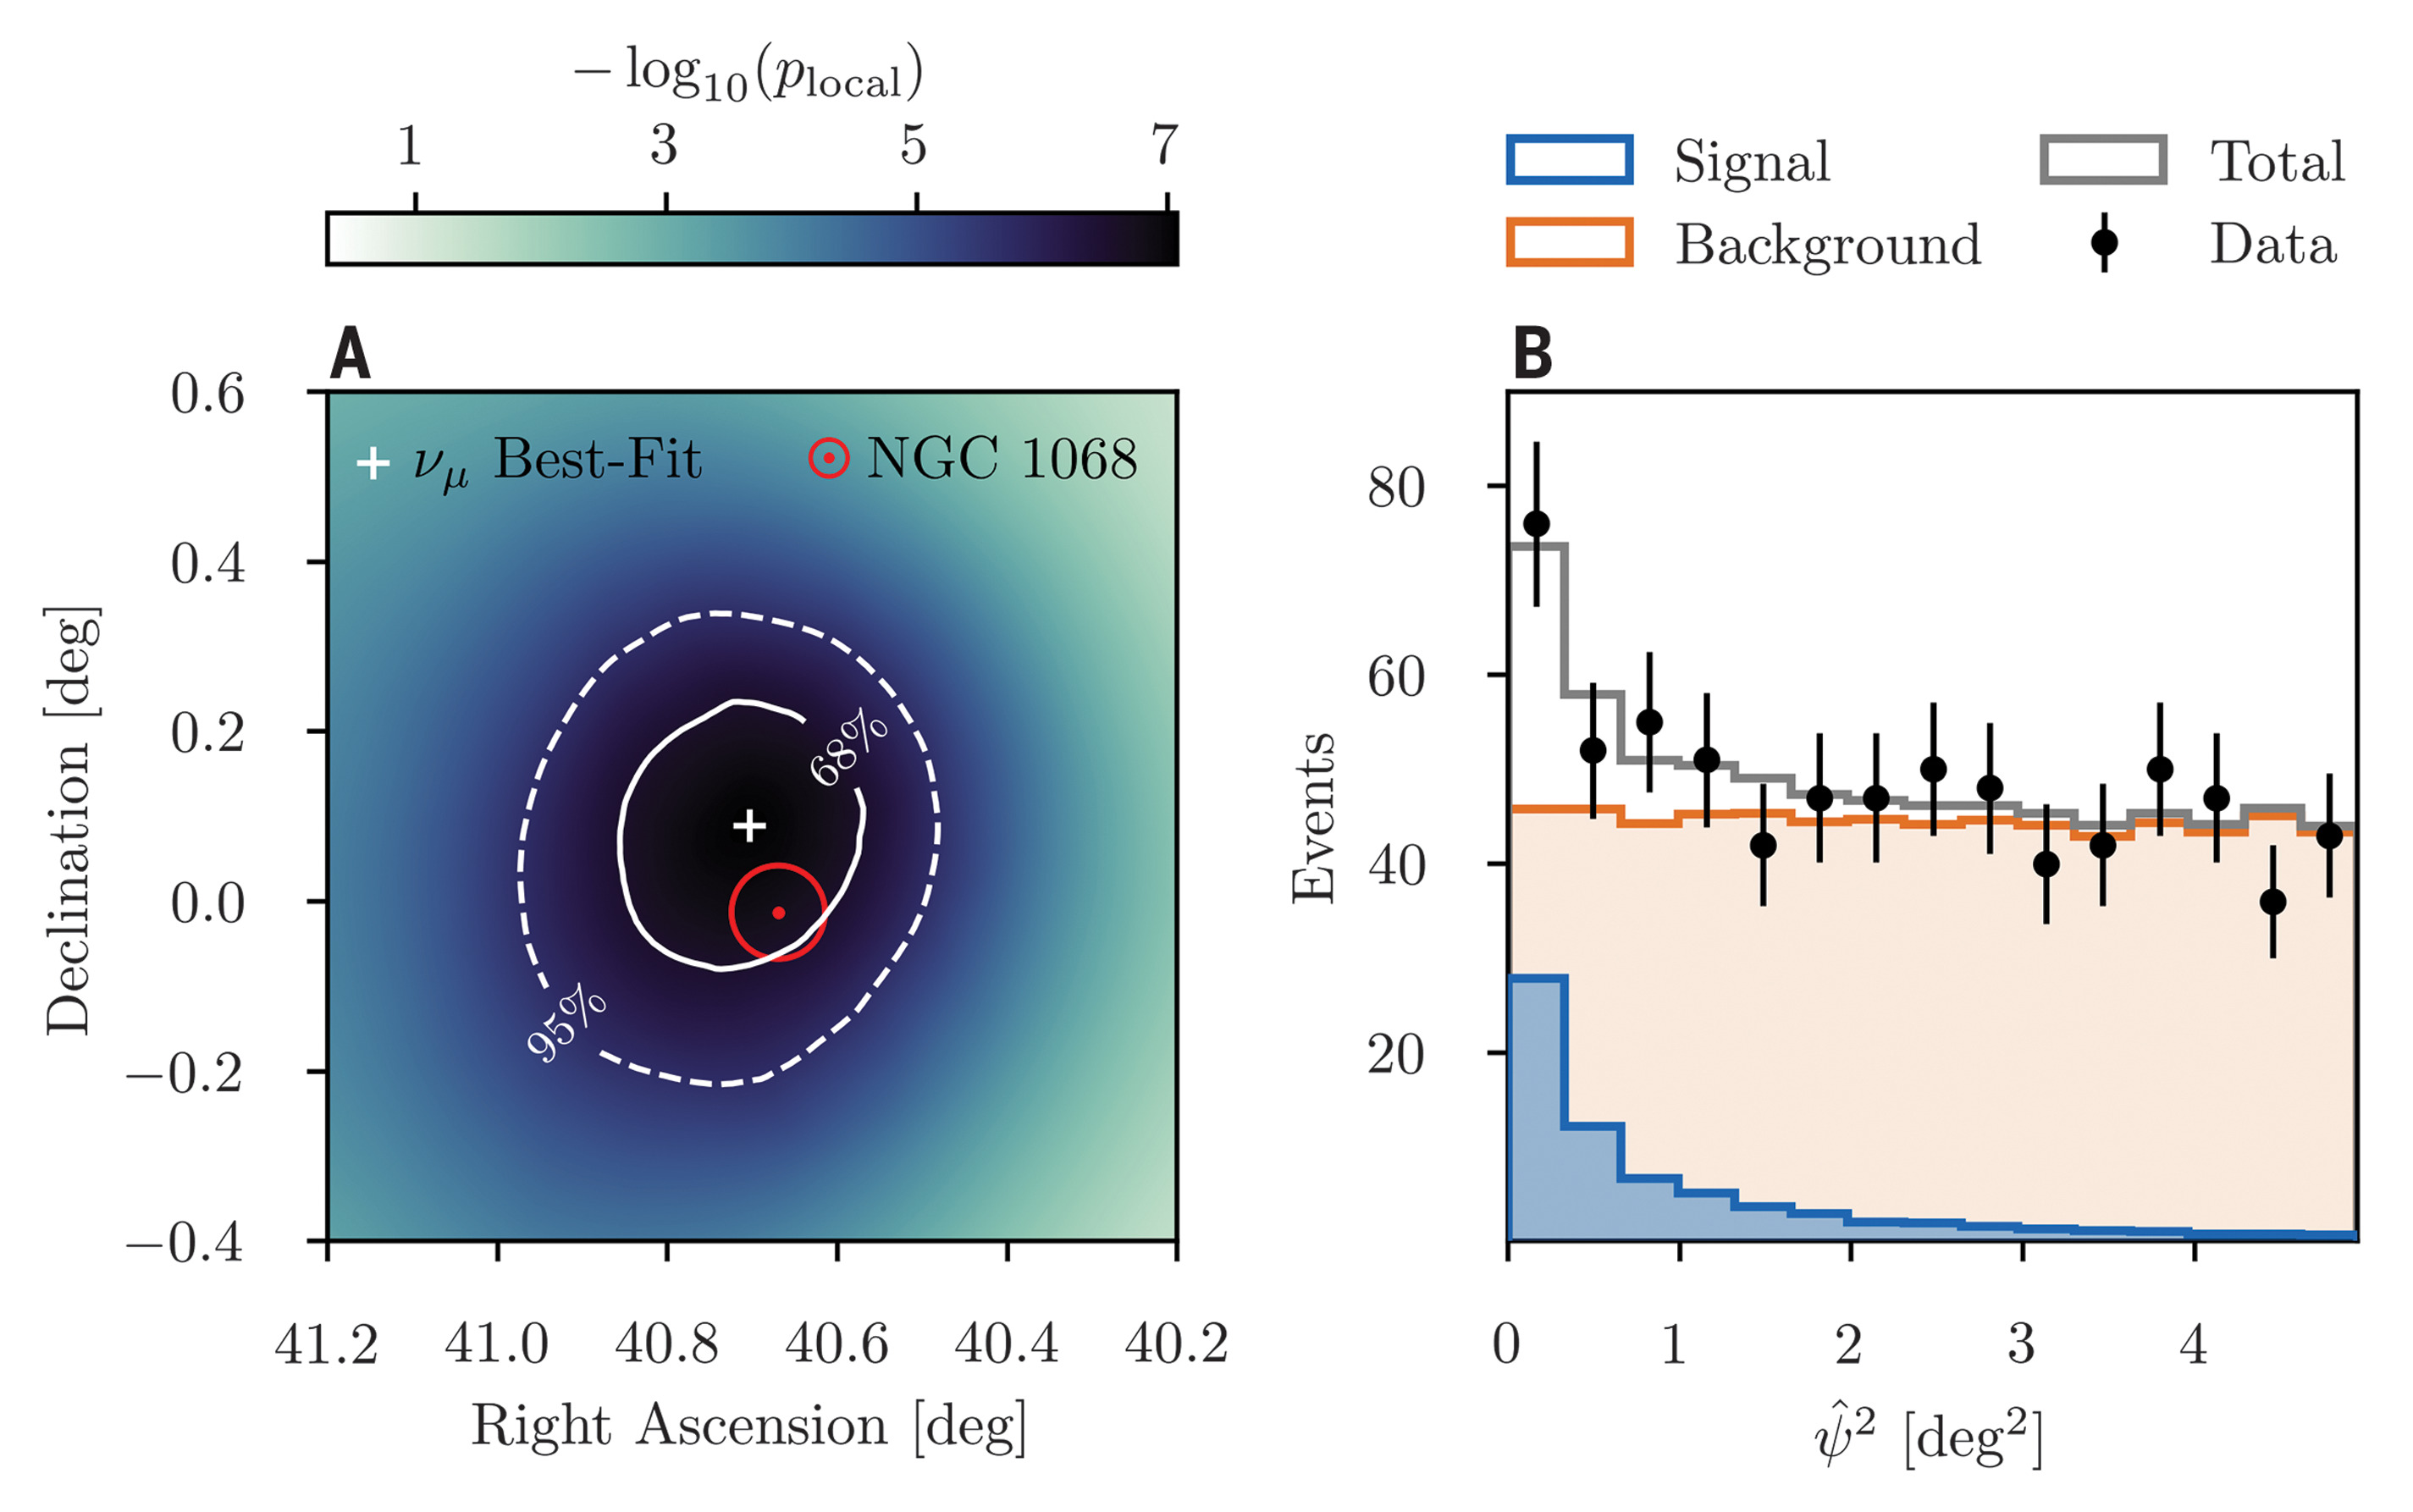
\includegraphics[width=14.5cm]{thesis_figures/CRnNu/science-abg3395-f2.jpg}
    \caption{Left:The sky region around the most significant neutrino excess spot in the Northern Hemisphere close to NGC 1068. The plot shows a fine scan of the region around the hottest spot. The hotspot is marked by a yellow cross and the dot marks the position of NGC 1068. Further, 
    the solid and dashed contours show the 68\% (solid) and 95\% (dashed) confidence regions of
    the hot spot localization. Right: The distribution of the squared angular distance between NGC 1068 and the reconstructed event direction. Taken from~\cite{Icecube_2022}}.
    \label{fig:NGC1068_excess}
  \end{figure}

  Since neutrinos arrive at Earth pointing directly back to their source, plotting the candidate astrophysical neutrino events measured by the neutrino telescopes over a sky map can localize their sources of origin. Such studies have been performed by various neutrino telescopes such as ANTARES~\cite{Albert_2021}, AMANDA~\cite{Abbasi_2009_Amanda}, BAIKAL-GVD~\cite{Allakhverdyan_2023} and IceCube~\cite{Icecube_2022}. Only IceCube has found the most significant excess of 81 events in the TeV range, arriving from the region within 0.18 degrees of active galaxy NGC1068 (M77). The Fig.~\ref{fig:NGC1068_excess} taken from~\cite{Icecube_2022} shows the hottest spot along with the excess. The association of the observation to the particular source has a significance of $4.2\sigma$. Hosting an active AGN surrounded by a dust torus makes it one of the ideal candidates for neutrino production~\cite{eichler1979high,berezinsky1981high}. The same analysis has also pointed out other potential neutrino source candidates PKS 1424+240 and TXS 0506+056. The latter of these is also important in the context of multi-messenger physics and is discussed later. 

  \begin{figure}[t!]
    \centering
    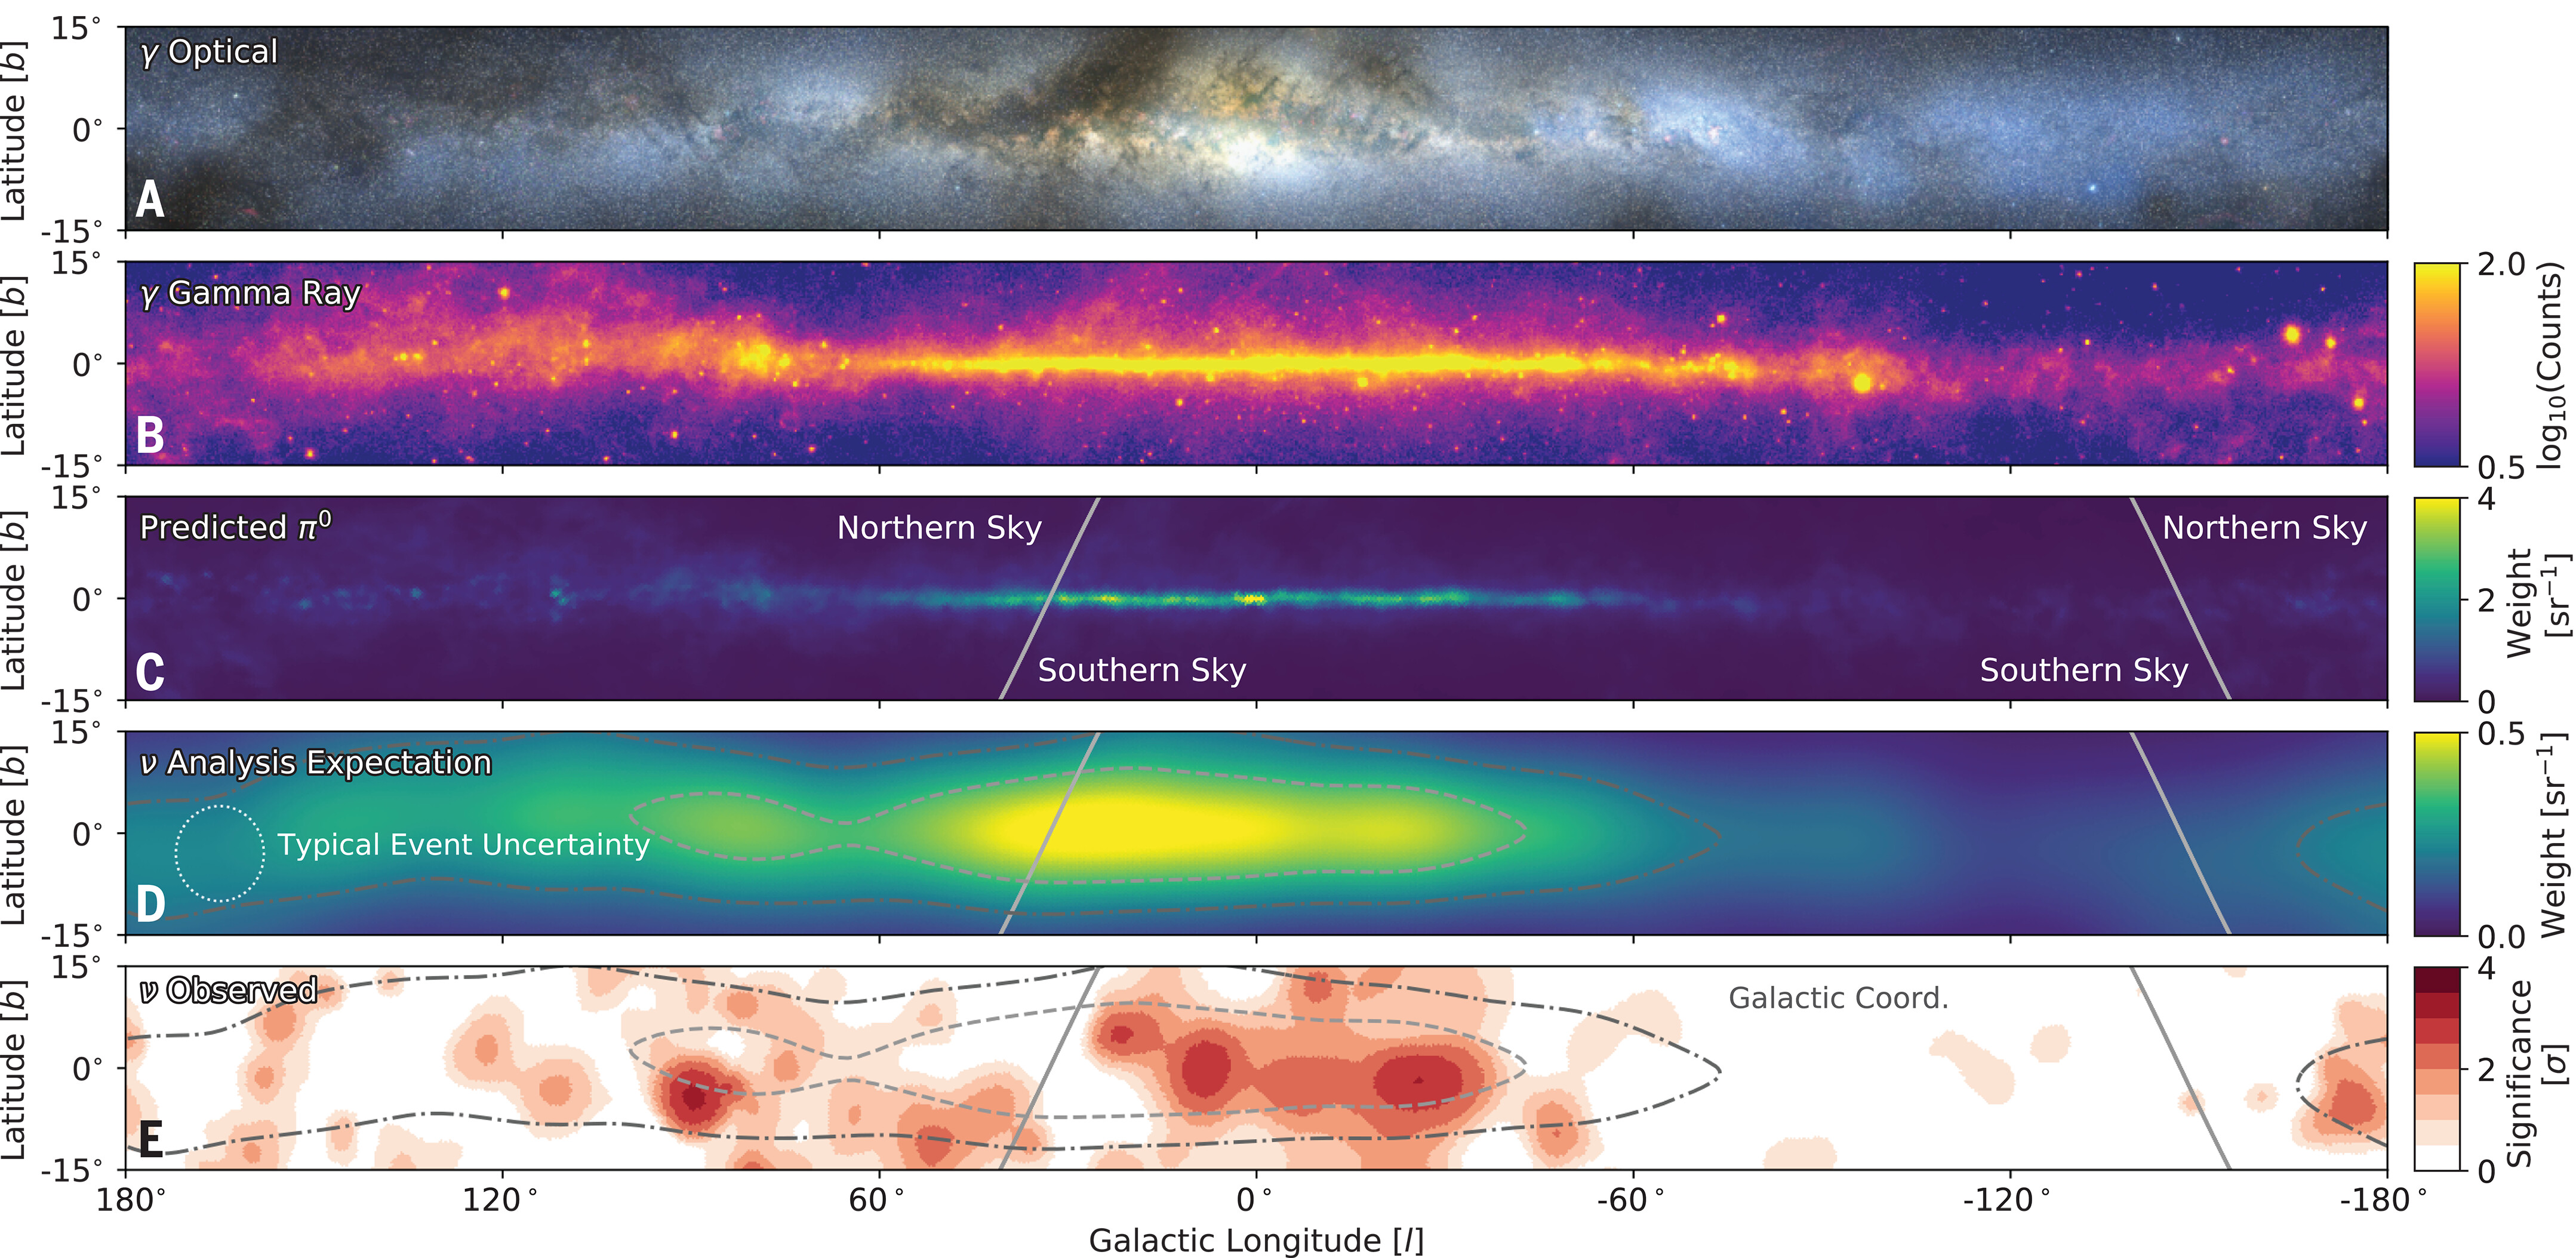
\includegraphics[width=14.5cm]{thesis_figures/CRnNu/science-adc9818-f1.jpg}
    \caption{Galactic plane with different messengers. The observation of neutrinos at the bottom is the final piece added to this picture. Taken from~\cite{Galactic_plane_nu_2023}}.
    \label{fig:Galactic_plane_nu_messengers}
  \end{figure}

  In 2023, IceCube also published the first observation of diffuse emission of high-energy neutrinos from the galactic plane of our own galaxy, the Milky Way~\cite{Galactic_plane_nu_2023}. The result is at the 4.5$\sigma$ level of significance when compared to a background-only hypothesis. However, the signal could also be due to a population of unresolved point sources near the galactic plane. This observation has opened a new way to observe our Milky Way galaxy and offers an evidence based proof confirming our understanding of both \gls{CR} and neutrino physics. It also opens a new avenue for the application of multi-messenger astronomy. The Fig.~\ref{fig:Galactic_plane_nu_messengers} shows the plane of the Milky Way galaxy as seen by different messengers.
  
\subsubsection*{Cosmogenic Neutrinos}

  \paragraph{Limits}
  \label{subsubsec:CosmoNuLimits}
  Both the Pierre Auger Observatory and the IceCube neutrino Observatory have also performed searches to look for UHE$\nu$s which have a cosmogenic origin. These searches have led to some of the most stringent upper limits for such fluxes. These limits are shown in Fig.~\ref{fig:Nu_limits_auger}. The results from the Pierre Auger Observatory dominate for energies above $10^{18}$eV and for lower energies, IceCube provides the best limits. The lack of observations can help constrain various models for high-energy neutrino production. These results can also help better our understanding of \gls{CR} physics and in particular their composition. The lack of observation of the expected neutrino flux predicted by a pure proton composition scenario for \glspl{CR} is an important result in favour of mixed composition scenarios. This result further points towards the spectrum cutoff being more likely due to a maximum rigidity limit for the sources rather than a GZK limitation. The detection of cosmogenic neutrinos can help complete the picture of the neutrino and \gls{CR} sky. 

\begin{figure}[t!]
  \centering
  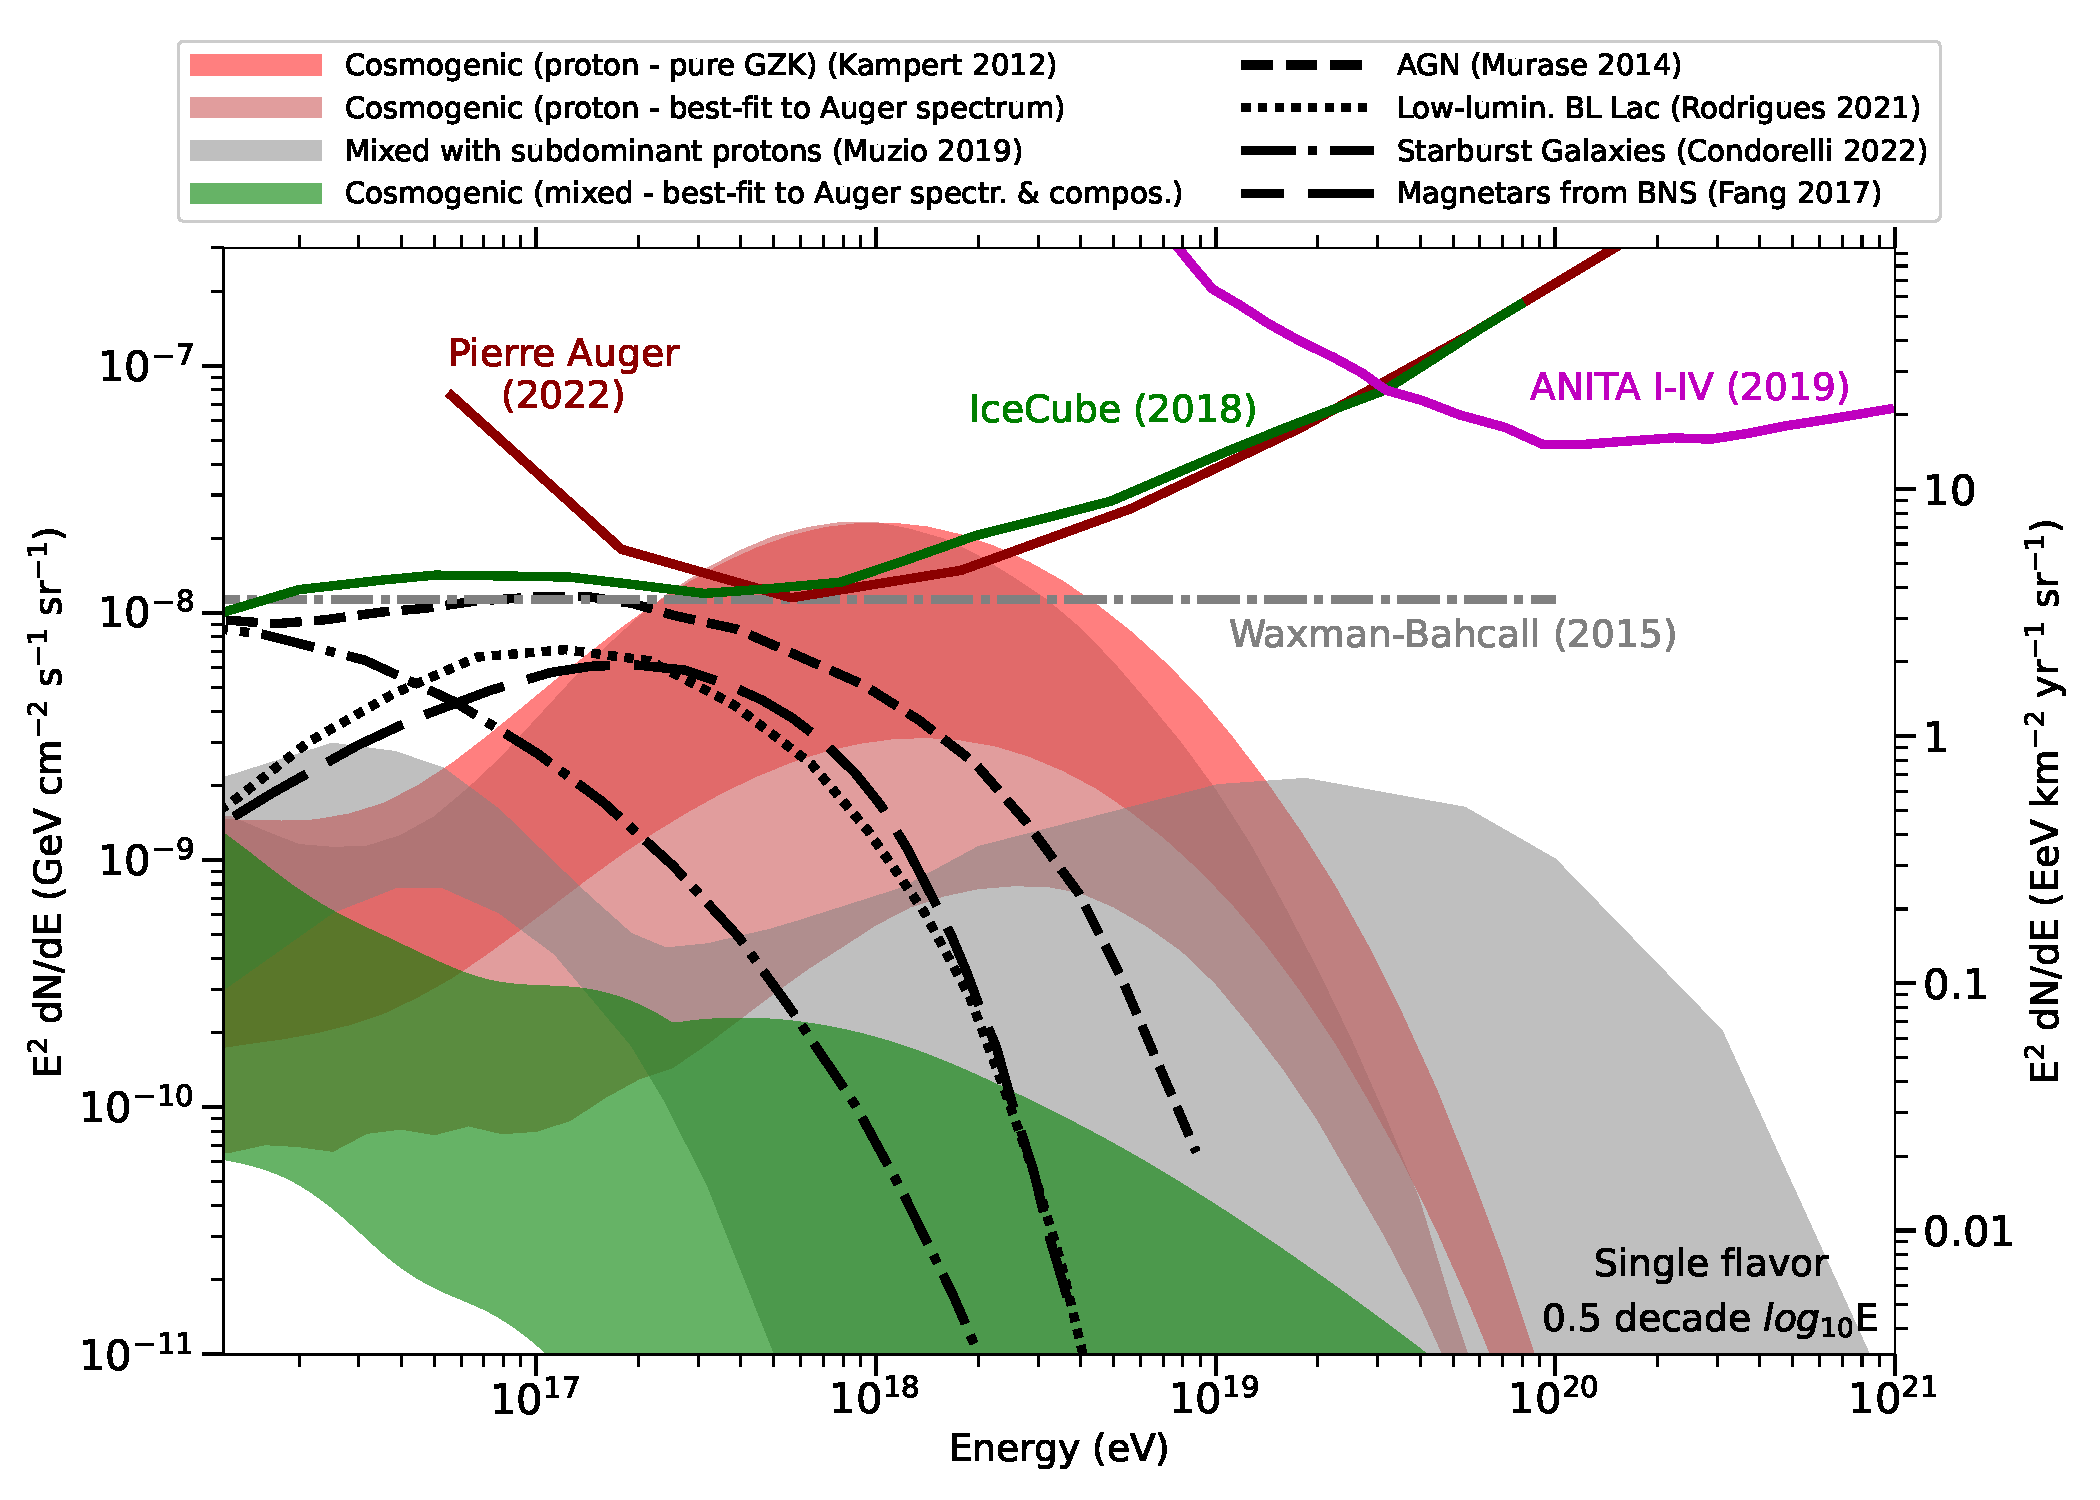
\includegraphics[width=14.5cm]{thesis_figures/CRnNu/neutrinolimits_icrc2023_wiki.pdf}
  \caption{Current upper limits on the diffuse flux of neutrinos from different experiments. Only the differential limits are shown. Also shown are the expected neutrino fluxes from different theoretical predictions for comparison. Taken from~\cite{PierreAuger:2023pjg}}.
  \label{fig:Nu_limits_auger}
\end{figure}

\section{Multimessenger Astronomy}
  \label{sec:Mul-mes}
Combining the various messengers via which we can see the Universe can help better understand the mechanisms behind their production and propagation. By combining the observations of various dedicated experiments for gravitational waves (LIGO/VIRGO), Gamma rays (FERMI-LAT, CTA), neutrinos (IceCube) and \glspl*{CR} (TA, Pierre Auger Observatory) a holistic overview of an astrophysical process can be gathered. The detection from one messenger/experiment and a non-detection from another can also be informative since it helps refine our understanding or might even reveal a new phenomenon~\cite{Abadie_2012,Albert_2017_GW170817}. One of the most important aspects of this field is a fast communication network via which all the different experiments can share their observations as fast as possible. Supernova Early Warning System~\cite{Al_Kharusi_2021}, established in 1999 and the Astrophysical Multimessenger Observatory Network~\cite{Smith_2013}, created in 2013 are some examples of the networks used in multi-messenger astronomy.  Some of the key observations of this field and the corresponding publications are summarized in table~\ref{tab:Multimessenger}. As mentioned in the introduction, the Pierre Auger Observatory continues to contribute to these searches~\cite{10.3389/fspas.2019.00024}. One of the best examples of this collaboration is~\cite{2022_spatial_corr_nu_cr} where a spatial correlation search for neutrinos and \glspl*{CR} was performed as a joint effort between ANTARES, the IceCube Observatory, the Pierre Auger Observatory and the Telescope Array. The GW 170817~\cite{Abbott_2017} multi-messenger analysis using more than 70 observatories cemented the benefits and the potential of multimessenger astronomy. 

\begin{table}[h!]
\centering
\small
\begin{tabular}{ |P{3.5cm}||P{2.4cm}|P{1.4cm}|P{1.9cm}|P{1.4cm}|P{2.4cm}|  }
  \hline
  \multicolumn{6}{|c|}{Multimessenger picture} \\
  \hline
  Astrophysical Event&Electromagnetic&Cosmic rays&Gravitational Waves&Neutrinos&Example\\
  \hline
  Solar flare   & yes    &yes&   - & - & -\\
  Supernova & yes    &-&   predicted & yes & SN1987a\\
  Neutron star merger & yes    &-&   yes & predicted & GW170817\\
  Blazar    & yes    & possible & - & yes & TXS 0506+056\\
  Active galactic nucleus & yes    &possible&    & yes & NGC1068\\
  Tidal disruption event& yes    & possible & possible & yes & AT2019dsg  AT2019fdr \\
  \hline
\end{tabular}
\caption{Current status of Multimessenger observations. Adapted from~\cite{Wik_mm}}
\label{tab:Multimessenger}
\end{table}

% \begin{figure}[t!]
%   \centering
%     \begin{minipage}[t]{.45\textwidth}
%       \centering
%       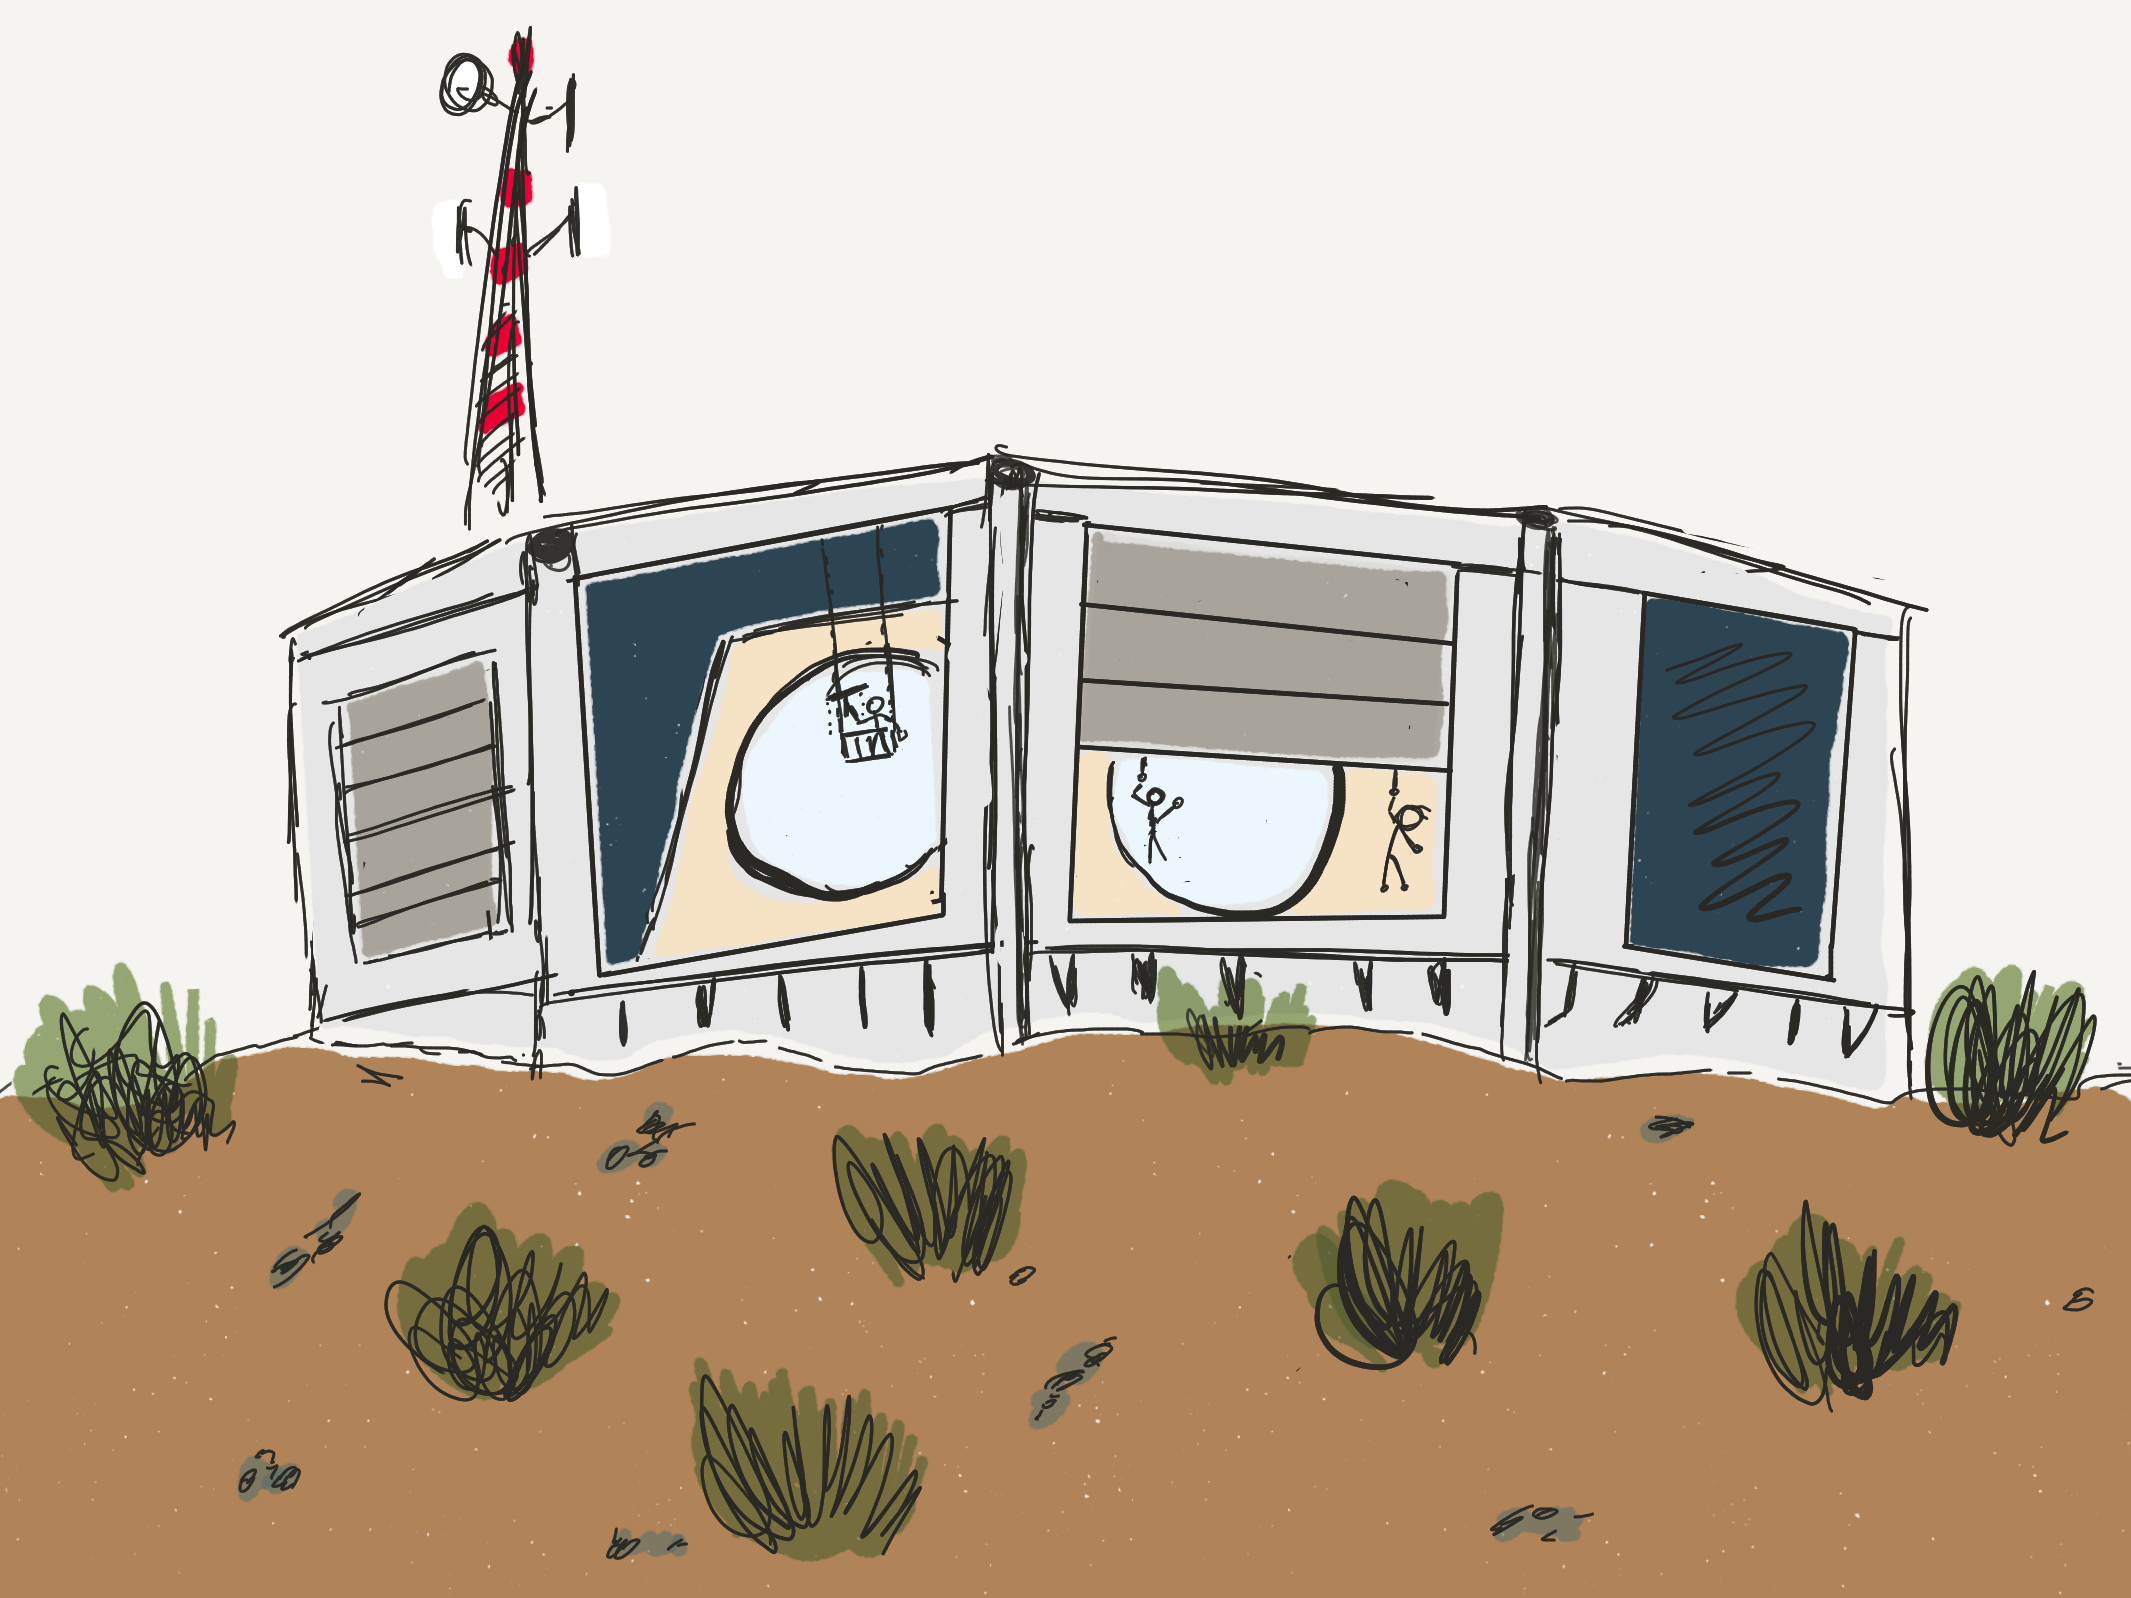
\includegraphics[width=\textwidth]{thesis_figures/Setup/FD_outside_drawing.png}
%       \caption{As artistic drawing inspired by the FD building at Los Leones.}
%       \label{fig:FD_sketch}
%     \end{minipage}
%     \hfill
%     \begin{minipage}[t]{.45\textwidth}
%       \centering
%       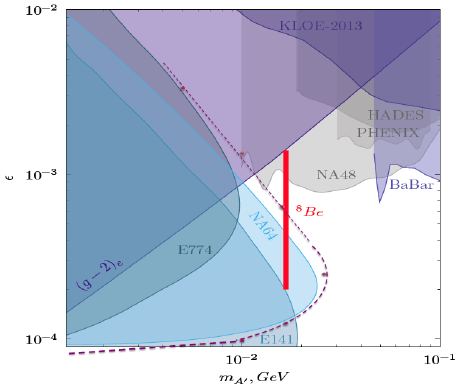
\includegraphics[width=\linewidth]{thesis_figures/exclusion_visible_latest.png}
%       \caption{Current limits for invisible mode for 90\% C.L. exclusion region in the ($m_{A'},\epsilon$) plane. The blue plane is with 2017 data and the dotted line is with 2017+2018 data for NA64. The red line is the region that might explain the X17 boson~\cite{}.}
%       \label{fig:exclusion_visible}
%     \end{minipage}
%   \end{figure}



%%% Local Variables:
%%% mode: latex
%%% TeX-master: "mythesis"
%%% End:

% !TEX root = mythesis.tex

%==============================================================================
\chapter{Extensive Air Showers}
\label{sec:EAS}
%==============================================================================

As mentioned in the previous chapter An Extensive Air Shower (EAS) is a cascade of high-energy particles that are produced when an ultra-high-energy cosmic ray, typically a proton or a nucleus, collides with a particle in Earth's atmosphere. This cascade can span over hundred to thousands of meters based on the energy of the initial particle and the incoming angle. EASs offer the best way to look for UHECRs since the low flux of these particles make direct detection using detectors mounted on balloons and spacecrafts not feasible. The EAS can be detected at the ground via an array of detectors. To infer the properties of the CR from the EAS it creates, one needs to model and understand how an air shower develops in the atmosphere. This chapter describes the process of the initiation and the development of the shower induced by CRs and neutrinos. It also aims to describe the important characteristics of EASs which help in extracting the relevant information and the last section is devoted to the detection of the EASs using different detector systems. 

\section{Development}
\label{sec:EAS_dev}
As the CR particle which is predominantely a proton collides with the nuclei of the atmosphere($N_2, O_2 $etc.) it produces pions and a few kaons. The neutral pions produced immediately decay to pairs of photons which in turn produce electrons via the process of pair-production. These electrons can then further produce photons via bremsstrahlung initiating a chain reaction which alternates between these two processes and forms the \textit{electromagnetic component} of the shower. The charged pions can survive for a while but eventually decay to muon and a corresponding anti neutrino. These muons can either survive till the shower reaches the ground and form the \textit{muonic component} or can also decay to electron thus contributing to the electromagnetic part. The neutrinos due to their low interaction cross-section mostly survive till they reach the ground and even further. Though not causing any problem for an EAS detector such neutrinos are the biggest background for a neutrino telescope. Kaons and charged pions due to their long lifetimes can also interact with the atmospheric nuclei producing additional pions which form the \textit{hadronic component} of the shower. The hadronic component can further contribute to both the electromagnetic and muonic component as more the shower propagates lesser the overall hadronic component becomes. A schematic of all the reactions with the different components is presented in fig~\ref{}.

The model the cascade of particles a detailed modelling of each component is required. These models help extract the basic properties of the cascade. A simplified model describing the electromagnetic component called the Heitler's toy model~\cite{} its hadronic extension and a general cascade equation are all discussed below. The specific development of a neutrino induced EAS is also discussed.  

\subsection*{Heitler's Toy Model}
\label{sec:Dev_Heitler}

Proposed by Heitler in 199~\cite{}, Heitler's Toy Model is a simplified perfect binary tree to understand and model an EAS development. The model characterises an EAS as a perfect binary tree. In such a scenario all particles produced in a shower equally share the primary energy available at the time of their creation. At each step which has a fixed size related to radiation length of the medium $\lambda$, the number of particles is supposed to be doubled with each having the same energy. The energy loses which may occur due to collisions are completely ignored. The shower development or splitting process is supposed to continue till a critical point where the energy required to create more particles becomes the same as energy lost by particles in the medium. At the critical point the shower has the maximum number of particles given by $N_{max} = E_0/E_c$ which is the ratio of the original energy to the critical energy. After this point the shower keeps getting absorbed in the atmosphere. The radiation length at this point is called the shower maximum denoted by $X_{max}$. This can be calculated to be $X_{max} = X_0 + \lambda_r ln(E_0/E_c)$ where $X_0$ is the first interaction point in the atmosphere. A visualisation of the shower development according to the Heitler's model is shown in fig~\ref{}.

Such a simplified model works quite well for estimating the properties of the electromagnetic cascades although the $N_{max}$ estimations do not match perfectly. The reason for this is the difference in the energy loss values for electrons and photons. For hadronic cascades an extension to the model was made. Other important properties of the shower such as lateral and longitudinal spread also requires to take into account the emmittance direction and losses due to collision which are not taken into account for a simplified model. These are discussed in sec~\ref{}. Even with its shortcomings the Heitler models gives a very good estimation for electromagnetic cascades and helps clearly categorise an air shower into three phases, the growth phase, the critical point phase and the tail phase. 

\subsection*{Hadronic Extension}
\label{sec:Dev_Had}
The Heitler model was extended by Matthews~\cite{} to characterise the hadronic cascades in an EAS. In his approximation when a hadron with Energy E interacts with a nucleon the total particles produced have a two-third charged component(charged pions) and a one-third neutral component with the initial energy equally divided based on the number fraction. The neutral component decays quickly and contributes its share of energy to the electromagnetic component. The charged hadrons, provided they have not reached their critical energy in air(~20 GeV), interact again repeating the initial process. Muons are only produced when the charged hadrons acquire an energy below the critical energy. The energy transfer for each component after n generations is given as $E_{had} = \biggl(\frac{2}{3}\biggr)^n E_0$ and $E_{em} = \big[1- \biggl(  \frac{2}{3}\biggr)^n\big] E_0$. Deeply penetrating air showers i.e a primary having a high energy and a low enough crossection in air results in a lower number of muons produced and observed at ground and a primary having a high cross-sections vice versa. This fact is important as based on the number of muons to electrons observed at ground can help estimate the type of primary. The number of muons can be estimated in this model directly from charged hadrons when their energy reaches blow the critical energy. For n generations $N_{\mu} = n_{ch}^n$ where $n_{ch}$ are the number of charged hadrons and n can be written as $n = \frac{ln(E_0/E_c)}{ln(n_{tot})}$. Generalising by eliminating generations:

\begin{equation}
    N_{\mu} = \biggl(\frac{E_0}{E_c}\biggr)^{\alpha} , \alpha = \frac{ln n_{ch}}{ln n_{tot}}
\end{equation}

All the parameters in this model need to be estimated using detailed simulations~\cite{}. $\alpha$ has been estimated to be in the range 0.82...0.9. Other factors such as production of particles which do not decay such as baryon-anti-baryon pairs~\cite{} can also affect the calculated values in this model. Other than the shower maximum and number of muons, the change of the depth of the shower maximum per decade in energy~\cite{} also called the elongation rate is given by $D_{10} = \frac{\left\langle X_{max}\right\rangle }{dlog_{10}E_0} = 2.3\lambda_r$. The elongation rate of electromagnetic showers in air is about $\approx 85g/cm^2$. The elongation rate theorem ~\cite{} states that the elongation rate for hadronic showers is also $D_{10}^{em}$ in the presence of Feynman scaling.

Another popular model to explain the development of air showers in particular the interaction with the nucleon is the superposition model~\cite{}. In this model a nucleus with mass A is assumed to be a superposition of A independent nucleons each with energy $E_h = E_0/A$. With such an assumption one can reach the following conclusions:

\begin{description}
    \item $N_{em,max}^A(E_0) = A N_{em,max}^h(E_h/E_c) \approx N_{em,max}(E_0) $ i.e the fraction of energy transferred to the EM component at shower maximum has only an indirect dependence on mass via the dependence on primary energy.
    \item $X_{max}^A(E_0) = X_{max}(E_0/A)$. This shows how the shower maximum has an inverse dependence on the mass of the primary i.e a shower initiated by heavier nuclei will develop higher in the atmosphere compared to one initiated by lighter nuclei.
    \item $N_{\mu}^A(E_0) =  A \biggl(\frac{E_0/A}{E_{c}}\biggr)^{\alpha} = A^{1-\alpha} \biggl(\frac{E_0}{E_c}\biggr)^{\alpha}$. This shows that heavier primaries will produce a larger number of muons compared to lighter primaries. For e.g. Iron showers contain 40\% more muons than proton showers~\cite{}.
    \item $D_{10} = D_{10}^{had} \Biggl(1- \frac{d\left\langle ln A\right\rangle}{dlogE}\Biggr)$ Since Feynman scaling is known to be violated for higher energies thus the hadronic elongation rate is always less than the electromagnetic rate. Thus, an increase in elongation rate towards 85 g/$cm^2$ is a direct indication of change of the mass composition. 
\end{description}
Simulations have shown that the superposition model gives a more realistic description of many features of the shower ~\cite{}. However, it is still not a perfect description especially for heavier nuclei. Studies with photographic emulsion techniques have tried to create a better picture of the fragmentation of heavier nuclei~\cite{}. This field is continuously evolving with better models and theoretical predictions being worked on based on our continually increasing database of observations. 

Although these models help to understand the principle a full Monte Carlo simulation and a generalised analytical solution of the cascade equations is needed to fully recreate the EAS. Even after such an effort a few discrepancies such as the muon puzzle which is the mismatch in the number of muons predicted by the simulations in comparison to the measurements~\cite{}.  

\subsection*{LPM effect}
Another process that can directly impact the development of high energy electromagnetic showers since it is the reduction of the bremmstrahlung and the pair-production cross-section is the Landau–Pomeranchuk–Migdal effect~\cite{}. All the above models work under the assumption that the energy range is low enough for the LPM effect to not be applicable. If the medium is dense enough or at high energies the LPM effect also becomes important to fully estimate the development of an air shower. The implications of the LPM effect for air showers implemented in simulations can be found in ~\cite{}. \todo{alexander citation}

\subsection*{Neutrino induced EAS}
\label{sec:Dev_Nu}
The development of a neutrino induced shower in comparison to a cosmic ray shower is important in the context of this study. Understanding the differences helps to identify the unique signature at a cosmic ray observatory like the Pierre Auger. The differences in the shower development can also help increase the sensitivity of a neutrino observatory like the IceCube.  Unlike a cosmic ray particle a neutrino can interact at any depth. This is due to the low neutrino cross-section at $10^{18}$ $\approx$ .. in comparison, for e.g. the proton-nucleon cross-section which is $\approx$ ... Thus, neutrino-induced showers require significantly higher neutrino energies to produce interactions with observable effects. The main channel via which an ultra-high energy neutrino can interact is either a CC or NC interaction. Neutrino-induced showers involve fewer particles in the initial interaction and often have a lower multiplicity of secondary particles compared to cosmic ray-induced showers. The development of the shower and the unique signature depend on the flavor of the neutrino as shown in fig~\ref{}.

An electron neutrino interacting via CC interaction produces an initial hadronic cascade which has fewer particles in comparison to a hadron-initiated shower from the CRs. The high energy electron/positron produced in the same initial interaction also produces an electromagnetic shower. At high energies the two showers are overlapped and depending on the fraction of energy carried by the electron/positron governs the ratio of the electromagnetic to hadronic component for the shower.

A muon neutrino also produces an initial hadron cascade but in contrast to the electron neutrino interaction the resulting muon has a very low probability to decay and mostly passes through the detector undetected. The energy carried by the muon which is usually a large fraction is lost and only the hadronic cascade can be detected.

Tau neutrinos have a unique and particularly interesting signature even among neutrino showers. The initial interaction remains the same with the production of a hadronic cascade, but the resulting tau lepton has a decay length $\approx$ 10km. This means that depending on the depth of the atmosphere the tau encounters on its way to the ground it can either decay and produce an electromagnetic cascade much later than the initial hadronic cascade or not decay at all. The asynchronous cascade signature is also known as "double-bang" effect and can occur both in air or a specific medium. Tau neutrinos can also be a source of upward-going air showers which can also be detected at an EAS detector. In this case the tau neutrinos can interact in the Earth's crust or in some natural obstruction like mountains around the detector leading to production of a hadronic cascade which gets absorbed and a tau lepton which can escape and produce an electromagnetic cascade in air that can be detected. The process is unique to tau neutrinos for an EAS detector since for the electron neutrino both the hadronic cascade and the electron is absorbed by the obstacle whereas for the muon neutrino the resulting muon is almost impossible to detect.  

All three neutrino flavors can also undergo NC interactions. These also result in an initial hadronic cascade and a neutrino which usually does not interact and escapes being detected especially for an EAS detector. Thus, the signature is indistinguishable in comparison to a muon neutrino CC interaction. The probability of NC interaction is also lower than a CC interaction which also affects the overall number of EAS induced due to this channel.

\section{Characteristics}
\label{sec:EAS_cha}
Apart from the shower maximum and the number of muons at ground other observables are also required to fully characterise the shower and estimate the important quantities such as the mass, energy and the arrival direction of the incoming primary CR or UHE$\nu$. Fig~\ref{} gives an overall picture of the evolution of an EAS in air. The amount of atmosphere penetrated is measured in units of slant depth X, with a unit of $g/cm^2$. The first interaction depth $X_0$ which is the slant depth until the first interaction of the primary particle with the nucleon. The shower begins from this point on and the vector along which the shower develops from the first interaction point is called the \textit{shower axis}. The development continues till the shower reaches a maximum which was defined earlier and is denoted by $X_{max}$. After this point the shower depopulates caused by particle energy loss due to absorption or decay. The \textit{longitudinal development profile} plotted in fig~\ref{} gives a relation between the number of shower particle in dependence to the atmospheric depth. This relation is also called the Gaisser-Hillas function~\cite{} parametrised as follows.

\begin{equation}
    N(X) =  N_{max} \biggl(\frac{X- X_0}{X_{max} -  X_0}\biggr)^{\frac{X_max-X_0}{\lambda}} exp\biggl(\frac{X_{max}-X_0}{\lambda}\biggr)
\end{equation}

$X_0$ and $\lambda$ can be estimated by fitting the profile based on the above function and depend on the composition and energy of the primary. $N_{max}$ is the number of particles observed at $X_{max}$. The integral of the longitudinal development profile gives an estimate of the total calorimetric energy deposited by the shower. 
The point where the shower axis vector intersects the ground is called the \textit{shower core}. Shower axis is thus defined by the zenith $\theta$, azimuth $\phi$ and the shower core position. If one looks at the shower head on the large thin disc like appearance consisting of highly energetic particles is called the \textit{shower front}. The shape is due to the path length differences between the shower particles travelling away from the shower axis to the one travelling in the direction of the shower axis. The disc is thus thinner near the shower core and widens away from it. As the shower front intersects the ground the density and the timing of the particles detected at the detector form what is called the \textit{shower footprint}. It is the primary observable used by a ground level EAS detectorto measure and characterise the shower. The arrival time of the particles in the footprint can help determine the shower geometry whereas the density can be used to reconstruct the energy of the primary. The density is estimated as a function of the radial distance from the shower core on the ground by the \textit{laeral distribution function}(LDF). The modern LDF function is an extension on the parameterisation given by Greisen~\cite{} and by Kamata and Nishimura~\cite{} and is given as:
\begin{equation}
    \rho_e(r) = \frac{N_e}{2 \pi R_M^2} C(s) \biggl(\frac{r}{R_M}\biggr)^{(s-2)}\biggl(\frac{r}{R_M}+1\biggr)^{(s-4.5)}
\end{equation}

with $s = \frac{3}{1+2 X_{max}/X}$ and the Moliere radius $R_M = 0.0265 X_0(Z + 1.2)$ \todo{Define other variables}. 


Another important characteristic of an EAS are its universality features~\cite{} first pointed out by Hillas for electromagnetic showers~\cite{}. In this formulation  around the shower maximum the average development of an air shower is universal. An individual shower can be defined as a function of shower age s give by:
\begin{equation}
    s = \frac{3}{1+2 X_{max}/X}
\end{equation}
Simulations have used such a universal feature to fit shower profiles reasonably well independent of the primary mass and energy~\cite{}. This feature is a result of the nature of the development of the cascade process which hides the initial primary dependent fluctuations~\cite{}. Air shower universality only holds for air showers induced by gamma rays, electrons, or positrons and breaks down for a hadronic cascade. It can still be used if each individual component of the shower can be disentangled. Although, not applicable for this study Universality is an important characteristic of the shower and has been used to estimate the proton-air corss-secton~|cite{} and other CR studies~\cite{}.

\section{Detection}
\label{sec:EAS_det}
At high energies due to the low flux EAS offer the best way to detect CRs. Low cost ground based detectors can be spread over large areas offering a cost effective way to study UHECRs. The shower can be seen through different emissions such as the Cherenkov, fluorescence and radio. The particles arriving at ground can also be directly detected. The different emissions which can be detected in context of EAS are described in this section along with an expected EAS signatures of a neutrino induced EAS which relates to the analysis presented in this thesis.

\subsection*{Fluorescence Detection}
\label{sec:EAS_flu}
The phenomenon of fluorescence emitted by air showers above $10^{17}$eV, known as "atmospheric fluorescence," involves the production of faint optical and ultraviolet (UV) light by the interaction of high-energy particles from extensive air showers with the nitrogen molecules in Earth's atmosphere. The energy levels of the nitrogen molecules determine the wavelengths of light that are emitted. The UV light emitted during the de-excitation process is typically in the near-ultraviolet range. The number of photons emitted directly correlates to the energy deposited by the shower particles. At altitudes between 5 and 10 km the yield has a height dependent rate of 4-5 photons per meter per charged particle. The photons can be seen at large distances up to 35km. The measurement of the light intensity through fluorescence telescopes with the help of the geometry of the shower axis offers a way to reconstruct the longitudinal profile of the shower and a subsequent energy estimation of the primary. Fluorescence telescopes are limited in their operational duty cycle which is about 10-15 \% since they can only be operated on clear moonless nights. A proper recosntruction of shower variables via the emitted fluorescence light also requires a constant monitoring of the atmosphere to account for light yield corrections. The pioneering fluorescence light detection of EAS include experiments at Volcano Ranch~\cite{} and Fly Eye experiment~\cite{}. Currently, this technique is also used at the the Pierre Auger Observatory and the Telescope Array.


\subsection*{Cherenkov Detection}
\label{sec:EAS_cher}
Charged particles moving through the atmosphere can also produce Cherekov light~\cite{}. The EAS can be either detected via Imaging Cherenkov telescopes(IACTs) which can detect showers between 20GeV -100 TeV and are used for gamma ray astronomy. For CRs non-imaging Cherenkov detectors can be set up akin to a ground based particle detector array. Since the cherenkov cone is collimated around the shower axis the detectors need to be located with small spacing between them. For eg. For a particle at 10km height The Cherenkov cone has a radius of 120m. This property and the similar operational limitations like the fluorescence detection make this a not viable technique to detect UHECRs. For UHECRs due to the low flux the a ground based Cherenkov detector array will require a very large number of detectors and will still only have a duty cycle of 10-15\%. The currently operational experiments using the non-imaging Cherenkov technique for EAS detection include Yakutsk~\cite{} and Tunka~\cite{} etc. IACTs are very popular for gammma-ray astronomu and multimessenger detections with H.E.S.S.~\cite{}, MAGIC~\cite{} and CTA~\cite{} currently operational. 

\subsection*{Radio Detection}
\label{sec:EAS_cher}
An EAS traversing through the atmosphere can also produce radio signals. The radio emission can be due to the geomagnetic field~\cite{} or the Askaryan effect~\cite{} described before. For air showers the emission due to the geomagnetic effect is supposed to dominate with the Askaryan effectonly contributing in the order of 10-15\%~\cite{}. This affect arises due to the deflection of electrons and positrons produced in the shower leading to the formation of an electron dipole moving through the atmosphere at the speed of light. This results in a forward focussed radio signal with a lateral distribution similar to Cherenkov emission. The radio signal depends on the orientation of geomagnetic field and the atmospheric conditions at the detector. Around 100 m from the shower core the expected frequencies are in the MHz range~\cite{} while near the shower core they are in the GHz range. For such frequencies and primary energies >$10^{17}$eV the emissions from the two different mechanisms is superimposed. The measured electric field scales with the primary energy of the shower.  Typically, to detect radio emission of an EAS several radio antennas are deployed over a wide surface area. These antennas are triggered by particle detector arrays. Self triggering is also being developed which will make the radi antennas a seperate functional unit for EAS detection. Some e.g. of currently operational radio antenna arrays for EAS detection include LOFAR~\cite{} and AERA~\cite{}. The Pierre Auger Observatory is also adding a radio antenna on each unit of their particle detector array which is supposed to become operational by 2024. Other planned experiments include GRAND~\cite{}. Neutrino observatories like RNO-G~\cite{} and IceCube-Gen-2~\cite{} could also potentially detect EAS.  

\subsection*{Particle detector arrays}
\label{sec:EAS_cher}
This is one of the oldest detection techniques used to measure and study cosmic rays. It consists of setting up a set of particle detectors spaced by large distances depending on the desired energy range sensitivity of the experiment which is also dependent on the altitude of the experiment. The detectors are usually arranged in a regular pattern, and they are able to detect the secondary particles of EAS at ground by searching for time coincidences between neighbouring stations. By measuring the signal and time delay between the triggered stations the incoming direction of the primary can be estimated to $1-0.5^{\circ}$ of resolution. The core position can also be determined by using the lateral distribution function to fit the recorded signal at the surface detector array. The energy can also be estimated through the measurement of number of muons at ground or cross calibration with other detector systems. Different types of detection methods have been used to combine and act as particle detector arrays. These include Geiger counters at MIT~\cite{}, hodoscopes at ...~\cite{}, scintillators at Volcano ranch~\cite{} and water or ice based Cherenkov detector. Currently scintillator based surface detector arrays and water/ice based Cherenkov tanks are the popularly used EAS detection techniques. 

Water/ice based Cherenkov tanks/detectors can also detect the secondary particles of EAS at ground. These are sensitive to the Cherenkov light which can be produced by these charged particles while travelling through the medium of the detector. The subsequent light is measured using a PMT~\cite{}. This ight signature is different depending on the type of the particle and thus can effectively help in differentiating between muons and electrons. The Pierre Auger Observatory uses an array of water Cherenkov tanks in conjunction with four fluorescence detectors for EAS measurements. IceCube also contains an array of ice based Cherenkov detectors which are used for cosmic ray studies and as a veto for their underground neutrino detectors. MOre details about the Pierre AUger Observatory are presented in chapter~\ref{}

Scintillator based particle detector arrays can be used to distinguish between the different secondary particles of an EAS. These consist of scintillating material which produced detectable photons if a charged particle traverses through the material. If deployed at the surface such detectors can act as excellent discriminators for electron and muons whereas if deployed underground they can only detect muons. The size of the scintillating material controls the zenith angle sensitivity which typically decreases the more inclined the shower is. TA uses a vast array of scintillator based detectors along with three fluorescence detectors to measure EAS. The Pierre Auger Observatory is also testing an array of underground muon detectors which are based directly below its surface array stations.


\subsection*{Towards detecting Neutrino Induced Extensive Air Showers}
Neutrino induced air showers have a particular expected signature. These showers are supposed to start much deeper in the atmosphere in comparison to ordinary cosmic ray showers, in particular proton showers which act as the primary background for their detection. The deeper interaction means less shower development till the shower front reaches the ground in comparison to a cosmic ray induced EAS. This difference in development can be measured by the muon to electron ratio at ground via a particle detector array. Since, the neutrinos are only expected to interact to induce a EAS if the volume of the atmosphere through which they traverse is large enough for zenith angles less than $60^{\circ}$ either the neutrinos are not expected to interact or and even if they do, due to the general amount of atmospheric volume at these angles the cosmic ray showers are supposed to be indistinguishable from a neutrino shower at least for a particle detector array at ground. This is due to the fact that the cosmic ray showers have not developed enough to lose the electromagnetic component of the induced EAS. This leaves the primary distinguishing factor i.e. the muon to electron ratio the same for neutrino and cosmic ray induced showers. The terminology used to determine the development of the shower in the atmosphere is the shower age and typically showers having a larger muonic component at ground are called \textit{old showers} while showers having a larger electromagnetic component at ground are called \textit{young showers}. 

Thus, to detect a neutrino induced EAS using surface detector arrays the smoking gun signal is an inclined ($\approx$ zenith angle > $60^{\circ}$) "young" shower. A perfect neutrino induced EAS detector should have a good angular resolution and a large electron-muon signal separation. However, this signature also not completely background free. Such a signature can also be caused by deeply interacting cosmic ray primaries or highly energetic muons emitting bremsstrahlung photons both of which can also induce a young shower. B meson could also be misidentified as a neutrino as shown in ~\cite{}. Other processes such as low energy showers coincident with a EAS could also act as background for a neutrino detection. These have been studied in detail in ~\cite{} and are negated in the analysis through the techniques developed in the reference. 
% !TEX root = mythesis.tex

%==============================================================================
\chapter{NA64 Experimental Setup}
\label{sec:setup}
%==============================================================================
\begin{figure}[h!]
\centering
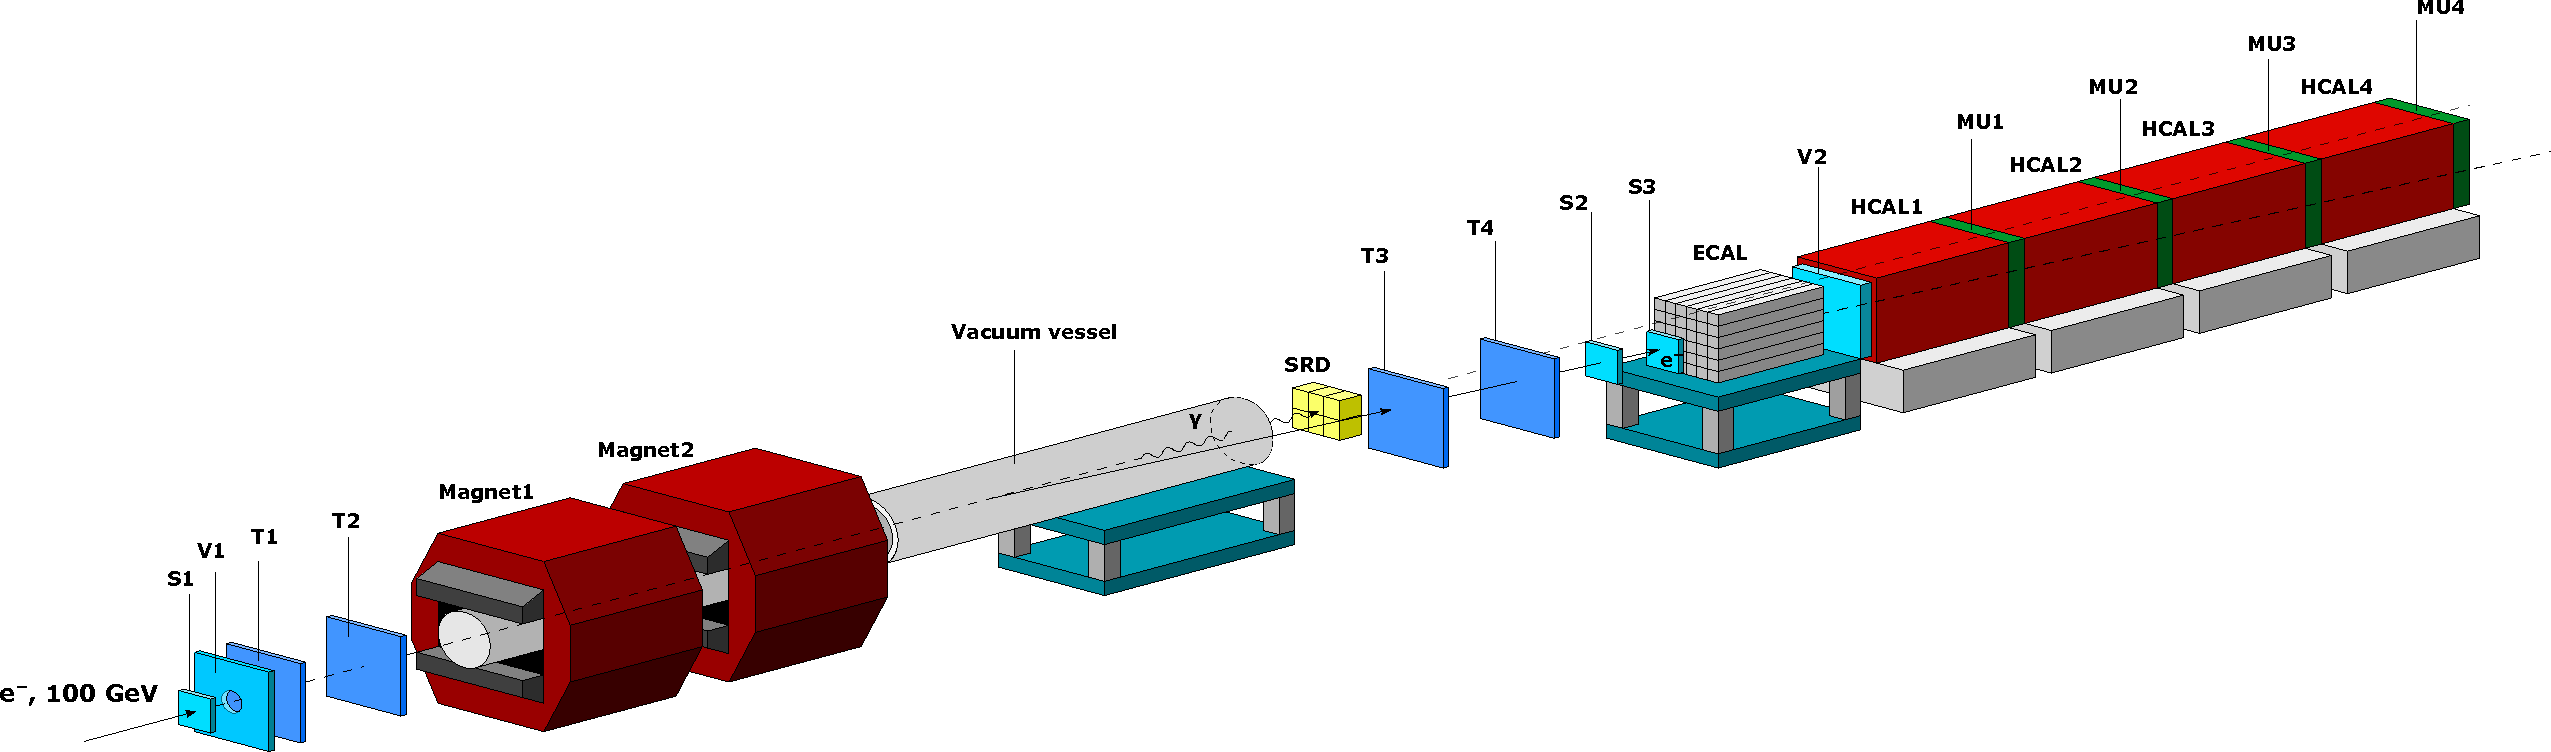
\includegraphics[width=\textwidth]{thesis_figures/Invisible_3d_setup.png}
\caption{Invisible mode setup~\cite{Banerjee:2016tad}}
\label{fig:Invisible_mode_setup}
\end{figure}

NA64 is a beam dump fixed-target experiment located at the H4 beam line of the Super Proton Synchrotron (SPS) at CERN. The objective of the detector is to look for rare dark matter candidates, primarily Dark Photons $A'$. $A'$ is supposed to be emitted via a process similar to bremsstrahlung $e^-Z\rightarrow e^- Z A'$. The experiment is not a permanent fixture and has been in operation since March, 2016. Since it's approval the setup has taken data a total of four times which included a two week test run in 2016 and four weeks of data taking each in 2016, 2017 and 2018. Each year the setup has slightly varied to account for different beam energies and expected background.

The SPS provides a primary proton beam of $400~\mathrm{GeV/c}$ with $\simeq 10^{12}$ protons per spill which is then converted to electrons by incidence on a beryllium target. The $e^-$ beam is in the momentum range $50-150~\mathrm{GeV/c}$ with a maximal intensity $\simeq 10^{7}$ per SPS spill of 4.8s. The provided high-energy $e^-$ beam with the large luminosity was needed since the $A'$ couples very weakly to the SM. The beam is then characterized by passing it through scintillators (S1-S3),veto ($V_1$), two dipole magnets with an integral magnetic field of $\simeq 7~\mathrm{Tm}$ and trackers (MM-section(\ref{sec:MM}), GEM-section(\ref{sec:GEM}) contained in tracking stations (T1-T4) which measure the $e^-$ beam momenta to a 1\% precision~\cite{article_beam_purity}. Additionally the combination of magnets followed by a 15m long vacuum vessel and a PbSc synchrotron radiation detector (SRD) acted as a filter to reject low energy electrons and hadrons that might be present in the beam and would contribute to the overall background. They were separated by putting a cut on the amount of synchrotron radiation energy deposited by the respective particle~\cite{Gninenko:2013rka}. The beam is then allowed to hit the electromagnetic calorimeter (ECAL) which acts as an active target. The ECAL consisted of 6x6 Shashlik-type modules each with 40 radiation lengths ($\mathrm{X_0}$) of which the initial 4$\mathrm{X_0}$ is employed as a separate preshower(PS) detector. The ECAL had a resolution of $\delta E_{ECAL}/E_{ECAL} \simeq 0.1 \sqrt{E_{ECAL}[\text{GeV}]}$~\cite{Banerjee:2016tad}.
The combined information achieved by studying the shower and the SRD signal helped in suppressing the hadron contamination in the beam to a remaining fraction of $ \lesssim 10^{-6}$~\cite{Depero:2017mrr}. A combination of Veto($V_2$) and hadronic calorimeter(HCAL) is situated downstream of the ECAL. They serve as a veto against muons, neutrals like high energy photons or hadrons produced in the target ECAL. The HCAL consisted of four modules ($\text{HCAL}_{1-4}$) separated by muon counters ($MU_{1-4}$) and were slightly shifted along the beam with each module consisting of 3x3 cells adding up to a total of $\simeq$30 nuclear interaction length ($\lambda_{int}$). The HCAL had a resolution of $\delta E_{HCAL}/E_{HCAL} \simeq 0.6 \sqrt{E_{HCAL}[\text{GeV}]}$~\cite{Banerjee:2016tad}.

\begin{figure}[t!]
\centering
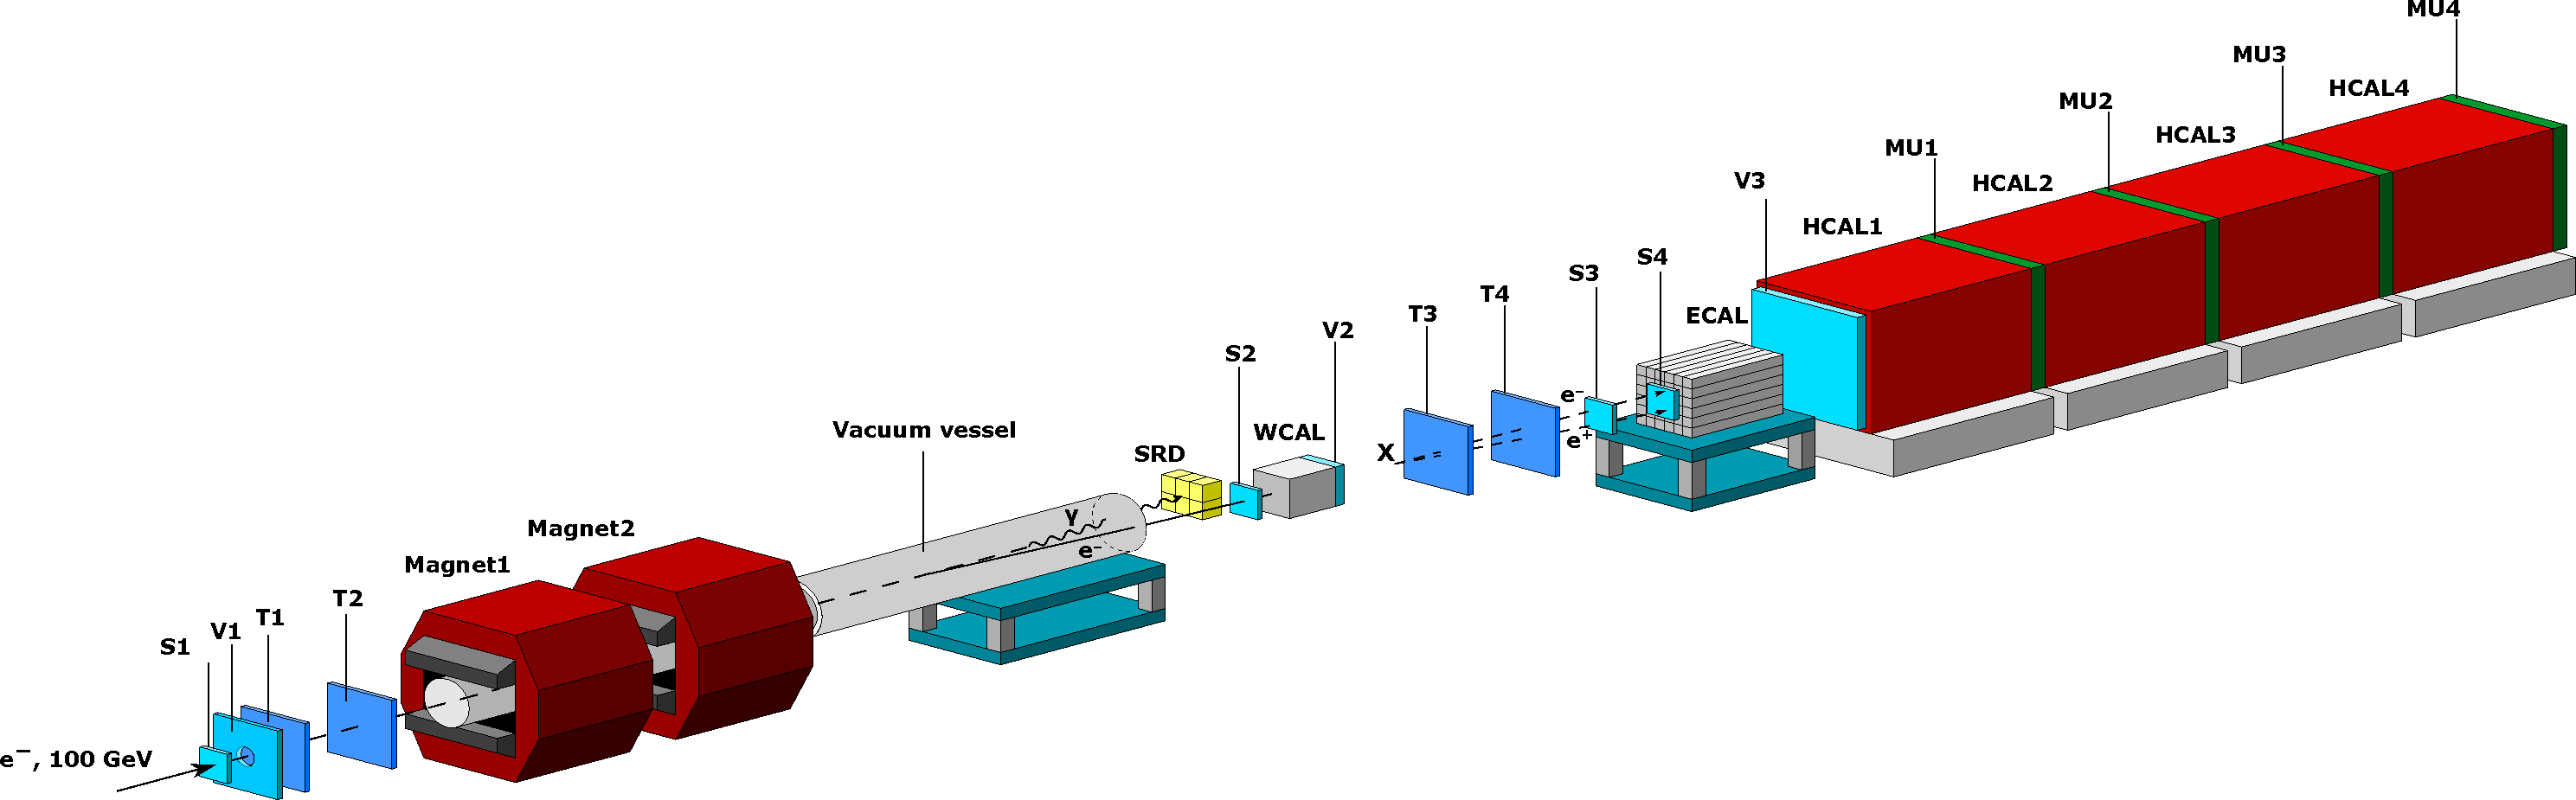
\includegraphics[width=\textwidth]{thesis_figures/Visible_3d_setup.png}
\caption{Visible mode setup 2017~\cite{Banerjee_2018}}
\label{fig:Visible_mode_setup}
\end{figure}

\begin{figure}[t!]
\centering
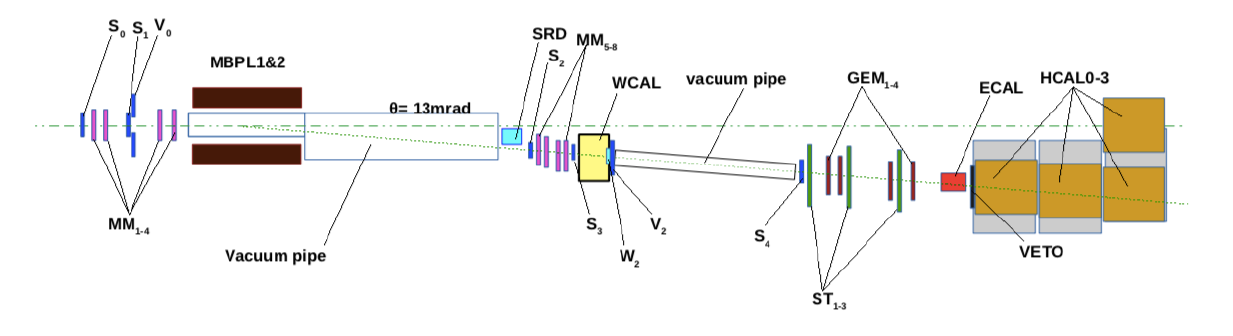
\includegraphics[width=\textwidth]{thesis_figures/visible_mode_newest.png}
\caption{Visible mode setup 2018-top view~\cite{Gninenko:2677228}}
\label{fig:Visible_mode_setup_side}
\end{figure}

The above setup works well for the \textit{invisible mode}($10^{-4} \lesssim \epsilon \lesssim 10^{-3}$, $m_{A'} \lesssim 1 \text{GeV}$) but requires modification for the search of $A'(X)$ in the \textit{visible mode}($10^{-4} \lesssim \epsilon \lesssim 10^{-3}$, $m_{A'} \lesssim 100 \text{MeV}$). To search for the visible decays a short tungsten calorimeter (WCAL) and a veto ($V_2$) were added right after the vacuum pipe and before the second set of tracking detectors (fig.(\ref{fig:Visible_mode_setup})). The size of the WCAL was selected so that the leakage of particles is small and the sensitivity to short lifetimes is maximized. The distance between the WCAL and the ECAL for the visible mode searches was slightly varied(2.5m->5.6m) between 2017 and 2018 which allowed for the installation of a 3.1m long vacuum tube to create better spacing between the ECAL and WCAL for a better angular resolution to increase the sensitivity to X17 bosons~\cite{Banerjee_2018}. A WCAL catcher was also installed in 2018 to prevent any leakage. Additionally the beam momentum was increased from 100GeV to 150 GeV in 2018 and one of the tracking station consisting of two MicroMegas (MM) was also shifted upstream of the WCAL. Counter ($W_2$) and straw detectors ($\text{ST}_{1-3}$) were also tested during the 2018 beam period(fig.(\ref{fig:Visible_mode_setup_side})). Both \textit{invisible} and \textit{visible} mode setups were also used to look for rare SM events that involve a photon decaying to a dimuon pair via bremsstrahlung $e^-Z\rightarrow e^-Z\gamma;\gamma\rightarrow \mu^{+} \mu^{-} $. Comparing these rare events, which were obtained from real data, to our Monte Carlo(MC) simulated sample helped in estimating the validity and efficiency of our MC simulation~\cite{Gninenko:2677228}.

In summary, NA64 tries to estimate and tag the beam $e^-s$ using a combination of trackers, SRD and ECAL/WCAL, uses the said ECAL/WCAL as an active target and then collects the residue of the interaction in the downstream HCAL/ECAL+HCAL. It also utilizes the hard bremsstrahlung photon to dimuon conversion as a measuring stick for the reliability of the MC simulations. The reactions of interest were attempted to be observed with a combination of hardware and software triggers depending on the expected signature of the decay mode for $A'$.

\textbf{Invisible Mode:}
$A'\rightarrow \chi \overline{\chi}$ signature:
\begin{flalign*}
  Beam(p\simeq 100~\text{GeV}),\\
  E_{ECAL+PS}(< 100~\text{GeV}),\\
  V_2(< E^{th}_{V}\simeq 1~\text{MIP}),\\
  E_{HCAL}(< E^{th}_{HCAL}\simeq 1~\text{GeV}).
\end{flalign*}

\textbf{Visible Mode:}
$A'\rightarrow e^+ e^-$ signature:
\begin{flalign*}
  Beam(p\simeq 150~\text{GeV}), \\
  E_{WCAL}(< 150~\text{GeV}), \\
  E_{WCAL+ECAL+PS}(\simeq 150~\text{GeV}), \\
  V_2(> E^{th}_{V}\simeq 1~\text{MIP}), \\
  V_3(< E^{th}_{V}), \\
  E_{HCAL}(< E^{th}_{HCAL}\simeq 1~\text{GeV}).
\end{flalign*}







%%% Local Variables:
%%% mode: latex
%%% TeX-master: "mythesis"
%%% End:

% !TEX root = mythesis.tex

%==============================================================================
\chapter{Neutrino Analysis $60^\circ < \theta < 75^\circ$}
\label{sec:DGL}
%==============================================================================
This chapter gives a brief summary of the neutrino search performed for the zenith range $60^\circ < \theta < 75^\circ$. The neutrino search is separated in different angular range to maximise the performance of the detector array in this case the SD for the search. The chapter aims to cover the expected signature in terms of measurable quantities in the Pierre Auger Observatory for the particular angular range, the neutrino simulation used to develop the analysis, the reconstruction chain used along with the quality cuts used for such an analysis. Further, the quality cuts are analysed in more detail especially in the context of improving the capability of the search by the usage of MoPS and ToTd. In the end the improvements to both the diffused and point source neutrino searches with the new triggers are quantified.


\section{SD Neutrino signature $60^{\circ} < \theta < 75^{\circ}$}
\label{sec:sig_DGL}

The strategy and method to detect neutrino showers in this angular range with the SD remains the same as mentioned before i.e to try detecting showers that develop late and have more electromagnetic or "young" shower front at ground. In terms of signal in the SD array the young shower is expected to be spread over a longer time period typically hundreds of nanoseconds and have a lower maximum peak compared to signal induced by older showers which are spread over tens of nanoseconds and have a higher maximum peak. A comparison of the difference between the induced SD signal from a young and old shower arriving from the same zenith angle is presented in fig. ~\ref{}. However, such differences in signals and the ability of the SD to differentiate between a neutrino induced and a proton/ heavy nuclei induced shower disappears for vertical showers($\Theta < 60^{\circ}$). For vertical showers a cosmic ray induced shower does not have enough time to develop because of the limited thickness of the atmosphere. At these zenith angles a high energy CR induced EAS can mimic the expected young shower signature of a neutrino induced EAS at ground. Thus, currently the neutrino searches at the Pierre Auger Observatory are limited to zenith angles above $60^\circ$ where it is much easier to separate a neutrino induced EAS from a CR induced EAS. Since we are also searching for young showers which have not fully developed till they are detected at ground, reconstructed energy cannot be used as a discrimination criterion.      

To select the longer signals in the SD one of the variables that was used in erstwhile neutrino searches is the fraction of ToT-T2 triggered signals in the recorded event. As mentioned in the previous chapter this trigger is tuned to select broader signals which for an inclined shower is evidence of a young shower. For the search presented in this thesis along with the ToT-T2, the ToTd and MoPS are also used. Both ToTd and MoPS as mentioned in sec.~\ref{} help further increase the selection efficiency for broader signals by reducing the impact of low energy muons. These muons which form the majority of the background at low zenith angles of the selected search range. Thus, these triggers are impactful in increasing the separation power for low energy($\leq$ 1 EeV) neutrino showers. Another important variable which is used to judge the width of the signals is Area Over Peak (AoP). The AoP is defined as the ratio of the integrated signal of the station over the biggest value or peak of the signal. The AoP is calibrated in such a way that narrow/ old shower signals have AoP ~ 1 while broad/old shower signals have AoP $\geqslant $ 1. 



\section{Neutrino Simulations}
\label{sec:sim_DGL}
To characterise the neutrino search ability of the Pierre Auger Observatory Monte Carlo simulations of EASs induced by UHE$\nu$s are required. There are six possible neutrino interaction chanels due to the three possible neutrino flavors with each having two possible channels(CC or NC). However, for simulations these are envisioned to be characterised by just two sets of simulations. For the NC channel since the EAS induced by three neutrino flavors has the exact same signature for our detector only $\nu_e$ NC simulations were performed to estimate the NC contribution of all the three flavors to the final exposure. 

For the CC interactions in the case of $\nu_{\mu}$ the resulting high energy muon has a high probability of evading detection. This is very similar to the NC interaction where the resultant secondary neutrino also carries approximately 80\% of the primary energy. Thus, after taking into account the appropriate crossection, in principle the NC simulations can be used to also estimate the contribution of $\nu_{\mu}$ CC channel.  

In the case of $\nu_{\tau}$ CC interactions where the resulting $\tau$ especially at higher energies($\geq $EeV) can decay and also initiate a secondary shower resulting in a "double bang" like signature in the Observatory. In the context of this thesis such signatures are not accounted for and the $\nu_{\tau}$ CC interaction is treated in the same way as the $\nu_{\mu}$ CC interaction resulting in a possible underestimation of the Observatory to $\nu_{\tau}$ events. A future $\nu_{\tau}$ simulation library is currently being prepared by the Pierre Auger Collaboration Monte Carlo task and could help extend this analysis in the future.

Thus, in summary $\nu_e$ CC and NC simulations can be considered to be good approximations to estimate the contributions of all the other channels to the overall exposure of the Observatory. The simulations were produced in two parts by the Pierre Auger Collaboration Monte Carlo task based on the GAP note ~\ref{}. The first part entails the simulation of the $\nu$ induced EAS in the atmosphere and the second consists of simulating the appropriate detector response for the corresponding shower. 

\subsection{Atmospheric Shower simulations}
\label{subsec:sim_EAS}
The first part included using CORSIKA~\ref{} to generate the EAS initiated by a $\nu$ primary. This involves simulating the primary neutrino-nucleon interaction which is performed in CORSIKA using the HERWIG code. Further options such as CHARM to track charm secondaries are not used. Also since only $\nu_e$ simulations are simulated, the TAULEP option which handles $\nu_{\tau}$ and $\overline{\nu_{\tau}}$ is also not used. The systematic uncertainties related to the primary interaction estimator is discussed later in section~\ref{}. CORSIKA further tracks the primary interaction products as they travel in the atmosphere towards the ground constituting the air shower. CORSIKA offers a wide variety of choice regarding selecting the hadronic interaction model. For the simulations used in this study separate high and low energy hadronic interaction models were used. For energies higher than 200 GeV three high energy hadronic models QGSJETT~\cite{}, SYBILL~\cite{} and EPOS-LHC~\cite{} were compared. The results of the comparison are mentioned in detail in Appendix~\ref{}. Since the differences between the models are not that significant for the neutrino analysis ....dash..... was chosen as the high energy interaction model. For lower energies FLUKA~\cite{} was chosen. The systematic uncertainities arising from different models are discussed in section~\ref{}.  

To account for the curvature of the Earth which is especially important for the zenith angles studied, the EGS4~\ref{} Monte-Carlo method is chosen to simulate the electromagnetic component of the shower. The analytical NKG~\ref{} method which is also available but is not used for these simulations since it vastly underestimates the maximum of the electromagnetic component due to the fact it does not account for a curved atmosphere. GDAS Malargue October atmospheric profile is chosen for the simulations and the magnetic field components are taken to be the default values at the Malargue site ($B_x = 19.52\mu T$ and $B_z = -14.17\mu T$). 

Further, since the computing times taken for shower simulations scale roughly with the primary energy, for primary energies > $10^{16}$eV these times become extremely long. Though parallel computing provides a viable solution, the technique of "thin sampling" or thinning~\cite{} offers an alternate way to reduce the computation times while simultaneously saving wastage of resources. The thinning algorithm is applied to all particles below the adjustable fraction of the primary energy which emerge from an interaction. Only one of these particles is followed ,and a proper weight is assigned to this particle to account for the untracked ones which are dropped based on the thinning level($\epsilon_{th} = E/E_0$). Additional improvements ~\cite{} which reduce the statistical fluctuation of particle densities far from the shower core using a maximum limitation of weights and reduction of number of particles close to the shower core where the detectors anyway have a high chance of saturation are also used as a part of thinning algorithm in CORSIKA. A thinning value of $10{-6}$ is used for the simulations in this study. An example of the CORSIKA input file used by the MC task to produce the simulated showers is shown below:

\todo{Add The CORSIKA steer file}

The simulations were performed using the GRID technology~\cite{}. Both CC and NC showers were simulated for fixed energy steps of log(E/eV) = 0.5 in the range $10^{17}-10^{20.5}$eV. The number of simulated showers was varied depending on the Energy, atmospheric depth of interaction and the injected zenith angle. More showers were simulated at lower energies and the energy dependent numbers are tabulated in table~\ref{}. Further, for both the interaction channels within the zenith angle range $60^{\circ}-70^{\circ}$ the neutrinos were forced to interact at fixed atmospheric depths in steps of 100 g cm$^{-2}$. The injection points both close to the ground where a neutrino shower might have a lower trigger efficiency and close to the top of the atmosphere where a neutrino induced shower might mimic one induced by a proton are rejected for the simulations. The azimuthal angle is left free and can take any value between 0$^{\circ}$ and 360$^{\circ}$. The simulated depths for each zenith angle bin are summarised in table~\ref{}. 

Based on (E,$\theta_{MC}$,X) bin the number of CORSIKA showers simulated vary. Higher values were chosen for lower energies to increase the statistics since at these energies the simulated shower has a higher chance of not being detected be the detector.  

After the simulation is completed CORSIKA produces a normal particle output file which contains information about the surviving particles on the ground level which is set based on the detector elevation. The file contains the relevant information such as energy, momentum, timing all segregated for each particle based on its Particle Data Group Code~\cite{}. It also produces a ".long" file which contains longitudinal distribution of various particle numbers along with the energy deposited which is relevant for fluorescence telescope based analyses. For this work the normal particle output files were used for further processing to simulate a response in the Pierre Auger Observatory SD.

\subsection{Surface Detector Response}
\label{subsec:sim_SD_resp}

The next step required to complete the $\nu$-induced shower simulation is to generate an appropriate detector response in the SD array for each simulated atmospheric shower. This is done using the Offline framework. The framework can read in the CORSIKA output files, undo the applied thinning, simulate the Cherenkov light which will be produced as the particles travel through the WCDs and then also mimic the corresponding WCD electronics outputting the trigger and event information for each simulated shower akin to how real showers are measured at the Observatory. Each step is performed using special modules. The module sequence used to simulate the detector response for $\nu$-induced showers in this thesis is given below: 

\todo{Add The module sequence}


The \textit{EventFileReaderOG} reads in the CORSIKA output file. The following steps are performed assuming an "ideal" SD array with every station operational and fully efficient within the design limts. The steps are also repeated for an individual shower between 5- 30 times depending on the primary energy to further increase the statistics for each (E,$\theta$,X) bin. The first module is the EventGeneratorOG sets the core position, time and event ID for Monte Carlo events. In this analysis similar to ~\cite{} the core position is only allowed to be randomised over a 5 x 5 km$^2$ area around a fixed station at the center of the array. This allows an in depth study of how core position could impact the reconstruction which is discussed later. In the next step the \textit{CachedShowerRegeneratorOG} reads in the list of the shower particles and unthins each particle injecting a set of new particles based on its unique weight~\cite{}. It can then create a list of particles for each SD station which is then passed to the next module \textit{G4TankSimulatorOG}. G4TankSimulatorOG uses Geant4~\cite{} to simulate the particle trajectories in the WCD and the corresponding Cherenkov light produced by these particles. It also handles all the possible absorption and reflection the light can suffer before it is measured by the PMT. Following this the \textit{} simulates the detector calibration constants described in section~\ref{} and the \textit{SdPMTSimulatorOG} takes in the information from the tank simulator and simulates a corresponding PMT signal(trace). \textit{SdFilterFADCSimulatorMTU} and \textit{SdBaselineSimulatorOG} further simulate the processing of the PMT signal by the electronics at each station with the first applying the filter response and the FADC sampling and the second adding baseline and simulated noise to these traces. 

The next two modules decide whether the simulated event fulfills the heirarichal trigger system of the Observatory explained in section~\ref{}. \textit{TankTriggerSimulatorOG} checks if the signal fulfills the local station criteria i.e T1 and T2 condition after which the \textit{CentralTriggerSimulatorXb} further combines all the station which fulfil the T2 criteria to form the T3 simulating the task performed by CDAS for real data. The \textit{CentralTriggerEventBuilderOG} and \textit{EventBuilderOG} then facilitate the transfer of events passing the T3 criteria from the simulation container class to the event class with the last module \textit{EventFileExporterOG} responsible for exporting all the processed showers now with the applied detector response in a file which can be further used for further reconstruction.  


\section{Shower Reconstruction}
\label{sec:reco}

The event reconstruction is a necessary step before any further analysis can be performed. This procedure is developed first for neutrino simulations to enhance their identification efficiency and then applied to real measured data for both estimating the possible background for a neutrino like events and for the final search for neutrinos at the Observatory. Shower reconstruction is also performed within the Offline framework with a module sequence that contains a combination of some standard reconstruction modules and some specific modules developed for neutrino identification in GAP note~\cite{}. The reconstruction is again performed with the help of the MC task on the GRID framework based on the particular reconstruction chain developed for neutrinos. The Module sequence used to reconstruct simulated neutrino showers is given below:

\todo{Reco modulesequence}

The sequence remains similar to the one used in~\cite{} apart from the iterative development performed by the Offline developers over the years. For data reconstruction the \textit{SdMonteCarloEventSelectorOG} is omitted from the sequence. The chain can be subdivided to three main parts which are "event reading and pre-selection," "angular reconstruction" and "posterior selection and export" which are discussed in the next few sections.

\subsection{Event reading and pre-selection}
\label{subsec:reco_presel}

The first module in this part of the reconstruction is again the \textit{EventFileReaderOG} which depending on the input format can parse the file. In the reconstruction sequence it is used to read in either the detector response simulated file for simulations or the measurement files obtained from the SD. The \textit{EventCheckerOG} further checks if the stations in each read event have proper timing information. After this point the FADC traces are processed with various modules to covert them to VEM units. The \textit{SdGainRatioCorrectorKG} corrects for the gain ratio for the electronics followed by \textit{TriggerTimeCorrection} which further corrects for differences in electronics especially related to timing for data over the course of its operation. The \textit{SdStationCheckerOG} further checks the station quality and appropriately sets silent stations if they do not contribute to the final trigger formation. After this point the \textit{SdHistogramFitterKG}, \textit{SdBaselineFinderKG} and \textit{SdTraceCalibratorOG} which get the calibration constants from the calibration traces, fit the baseline and the convert the traces to VEM units respectively. Further modules \textit{SdStationPositionCorrection} corrects the positional differences that might arise due to faulty GPSs which is important for correct timing information, \textit{SdBadStationRejectorKG} sets known bad stations in the array to be inoperational and the \textit{SdSignalRecoveryKLT} which tries to recover signals from the saturated PMTs if any by looking at the undershoot value~\cite{}. An extra module \textit{SdPMTQualityCheckerKG} is also used in the case of data reconstruction to estimate the quality of the detector.

The next three modules are used to fine tune the selection of signals and later events to improve the both the quality of simulated and measured data to increase the efficiency of neutrino detection. The first one is the \textit{SdEventSelectorOG} which applies a basic SD event selection which is also used in other analyses. The module sets conditions based on T4, T5 and other station based parameters if appropriate. The different operations performed by the module are as follows:

\begin{description}
  \item $\bullet$~\textbf{Bottom-up Selection:} This selection helps in deciding the non-participating stations if the stations are not compatible with a planar shower front propagating at the speed of light hypothesis~\cite{}. Such stations can arise due to random noise in the array or due to random coincidences between non-air shower events with air shower events. The selection requires a minimum of three stations which fit the planar front of the shower within lenient time tolerances. It also removes isolated stations by checking the distances to nearest neighbors. Though, the selection is applied, it is not very effective for inclined showers(>$60^{\circ}$) since the showers above these angles are not geometrically compact. Thus, this selection is supplemented with an extra top-down selection implemented in \textit{SdTopDownSignalSelectorUGR} which is discussed later. 
  \item $\bullet$~\textbf{T4 and T5 trigger:} The module also calculates the T4 and T5 criteria discussed in sec.~\ref{}. It also then further discards events if they do not fulfill these criteria. In this study the T4 criteria was not required but a stringent 6T5 criteria was required for the selection. 
  \item $\bullet$~\textbf{Lightning Rejection:} The lightning events can be detected in the SD stations by looking for oscillatory signal in the FADC trace of all three PMTs~\cite{}. For this analysis if any lightning like signal is detected in any one of the stations the whole event is rejected from the analysis. 
  \item $\bullet$~\textbf{ToTd and MoPs trigger:} The module can also silence particular triggers before applying the selection. This feature is used to produce two sets of reconstruction files one with the triggers turned off and one with them turned on. This can impact the number of events fulfilling the 6T5 conditions and thus the overall number of events which can be seen later.    
\end{description}

The \textit{MonteCarloEventSelectorOG} further removes stations with distance in shower plane coordinates smaller than the inner radius used in the CORSIKA simulations. It also removes dense stations i.e virtual stations which are sometimes used for MC studies since these are not representative of the regular SD array. 

The \textit{SdTopDownSignalSelectorUGR} is a module developed specially to carry out a top-down selection and accidental signal rejection for neutrino like events. A summarised overview of what this module aims to accomplish is given next with a detailed description of the module already published in ~\cite{}. The Top-down procedure is applicable for both the simulations and measured data whereas the accidental signal treatment is only applied for measure data. The procedure is based on~\cite{} and ~\cite{}. Top-down selection requires a minimal of three station with the shower front time tolerance compatibility dependent on the zenith angle. If the fit does not converge stations are successively removed and re-tested until a satisfactory fit is achieved. At the end of the procedure stations which do not contribute to the final fit are rejected while the others are marked as candidate stations. Further the Top-Down procedure also takes into account the individual traces and uses the shape for 3-fold topologies. It also rejects isolated signals akin to the Bottom-up selection but with larger tolerances to account for the wider footprint of inclined events. The module also applies an accidental signal rejection procedure before the top-down procedure is applied to account for the atmospheric muon background. The atmospheric muons and also local showers can either trigger isolated stations or even real event stations affecting the start times and in turn the zenith angle reconstruction. This miss-reconstruction can either cause problems with the fitting of the top-down procedure and can also lead non-neutrino like or background events pass the analysis cuts affecting the overall neutrino detection efficiency. The module discards stations with total signals below 3 VEM which rejects the muonic background which typically peaks at 1 VEM. The discarding procedure is implemented only till the minimal number of stations present in the event are below 6. 


\subsection{Angular Reconstruction}
\label{subsec:reco_presel}

The angular reconstruction forms the basis for neutrino detection using the SD especially since for inclined neutrinos the energy reconstruction algorithms typically used for cosmic rays at the Pierre Auger Observatory become unreliable. The angular reconstruction is performed by the \textit{SdPlaneFitOG} and \textit{LDFFinderKG}. The energy reconstruction using the SD is either typically done using the \textit{LDFFinderKG} which fits a lateral distribution function to the SD signal based on the NKG approximation. The NKG approximation is typically inaccurate for inclined showers above a zenith of $60^{\circ}$ thus alternate methods based on muon maps are used for inclined showers. These also fail for neutrino induced showers usually having a large electromagnetic component. Thus, without a reliable energy reconstruction angular reconstruction becomes vital for neutrino induced shower detection at the SD. 

The angular reconstruction procedure uses the timing information from the stations to fit either a plane or a spherical shower front. The axis of shower $a$ is initially assumed to intersect the ground at some time using a signal weighted barycenter $x_b$ and bary-time $t_b$ of selected stations located at $x_i$ with start time $t_i$ given by :




The choice of the weights taken as $\sqrt{S} $ with $S$ being the signal of the stations has been previously evaluated using Monte-Carlo studies~\cite{} to give the best results. The barycenter also serves as the first estimate of impact position of \textit{shower core} at ground but is later estimated more accurately. The shower core is assumed to be moving in the $-a$ direction. Under the plane-front assumption the particles in the shower front move in a plane perpendicular to the shower axis($shower plane$) with the same speed as the core of the shower which is the speed of light c, the time t(x) when the shower plane passes through some chosen point
x (e.g. a station on the ground) can be inferred through a simple projection onto the shower axis as,


Assuming a minimal change in altitude which is true for SD location and precise knowledge of station locations the deviations in estimating the geometrical shower parameters can be due to the uncertainity of the observed start times $\sigma_t$. Thus, the following function needs to be minimised to fit the model for the measured signal start times 


The start time variance needs to be modified for the new triggers and has been taken from~\cite{}. Replacing the axis with $a =(u,v,w)$ and the station coordinates with $x = (x,y)$ (ignoring altitude z). Adding the constraint $u^2 + v^2 + w^2 = 1$ the $chi^2$ can be easily solved. The solution only fails if the stations used while fitting have a linear dependence(three stations in a line) but for higher station multiplicity this is highly improbable especially for the theta range explored for the DGL channel. For more inclined events different solutions to the zenith estimation are used~\cite{}. 
 
Another shower front estimation technique based on a curved shower front approximation is also used to fit the measured stations~\cite{}. The reconstruction assumes the shower development starting at time $t_o$ from a point of origin $x_o$ propagating toward the ground as a concentrically expanding sphere with the speed of light, $c$. The arrival time can thus be estimated as:


As can be seen by the equation, the spherical fit is decoupled from any prior knowledge of the shower core or the shower axis. It is only dependent on the point of origin. Quantities such as shower axis can be determined later when the impact point has been estimated as $x_o -x_c/ x_o-x_c$. The expected solid angle differences between the two fits are of the order of half a degree. The curvature shower front fit is only used for station multiplicities greater than five. This is so because for lower station multiplicities the degrees of freedom are not enough to solve for the shower-front curvature(R-$\infty$). 


\subsection{Posterior selection and Export}
\label{subsec:reco_possel}

The last part of the shower reconstruction chain includes the application of the \textit{SdEventPosteriorSelectorOG} module which computes the 6T5 \textit{posterior} trigger differing from the 6T5 criteria mentioned earlier. The 6T5 posterior requires the 6 stations in the first crown from the nearest station to the reconstructed shower axis to be active or alive during the event. The events which do not pass this criterion are rejected. The last module \textit{RecDataWriterNG} exports all the relevant information to ADST~\cite{} files. In case of reconstructed simulations both the simulated and reconstructed information is stored while for measured data only the reconstructed information is stored.


\section{Reconstructed $\nu$ simulations}
\label{sec:reco_possel}
This section includes some sanity check to check and verify the quality of the $\nu$ simulations. Fig shows the  Efficiency of the reconstructed showers as a function of the zenith angle and the slant depth. The next figure shows the frequency of reconstructed events based on the core position. The non-uniform distribution with the minimal events for core positions close to the stations can be explained due to two reasons. The first being the removal of stations if the PMTs for the particular station is saturated. This saturation can occur for stations very close to the core. The second reason  



\section{$\nu$ selection}
\label{sec:nu_sel}
This section tries to describe the decisions made to select $\nu$ induced air showers. The selection is optimised and evaluated on the above-mentioned neutrino simulations and a part of measured data used as an estimate for the expected background. Since a \textit{blind search} strategy is envisioned for the search. The rest of the measured data forms the \textit{search sample} and will be used to look for neutrino like events during \textit{unblinding}. 
In the first part the selection used to select $\nu$ showers is described in more details. The selection consists of some pre-selection cuts applied to enhance the reconstruction quality of the selected events followed by a Fisher Linear Discriminant~\cite{} based on experimental observables which is the main criteria of differentiation between a $\nu$ induced air shower and background.  
In the second part the performance of the selection is further evaluated based on temporal changes such as aging in the surface detector along and the neutrino detection efficiency is quantified. Comparison to previously used selection are also discussed especially in the context of the performance improvements achieved by using new triggers for neutrino detection.

\subsection{Samples Used}
\label{subsec:nu_sel_samp}



\begin{figure}[t!]
\centering
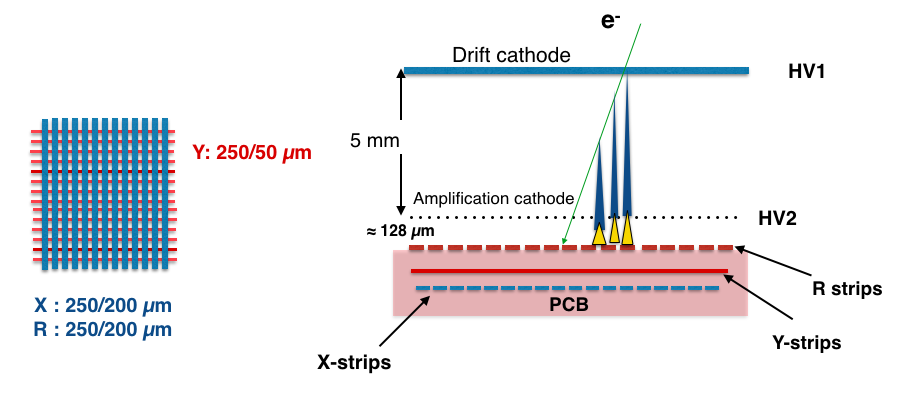
\includegraphics[width=\textwidth]{thesis_figures/NA64_MM.png}
\caption{Left: Strip dimensions of the modules, Right:NA64 Micromega's working principle~\cite{Banerjee:2017mdu}}
\label{fig:Micromegas_na64}
\end{figure}

\subsection{Gas Electron Multiplier}
\label{sec:GEM}

 \begin{figure}[t!]
 \centering
   \begin{minipage}[t]{.45\textwidth}
     \centering
     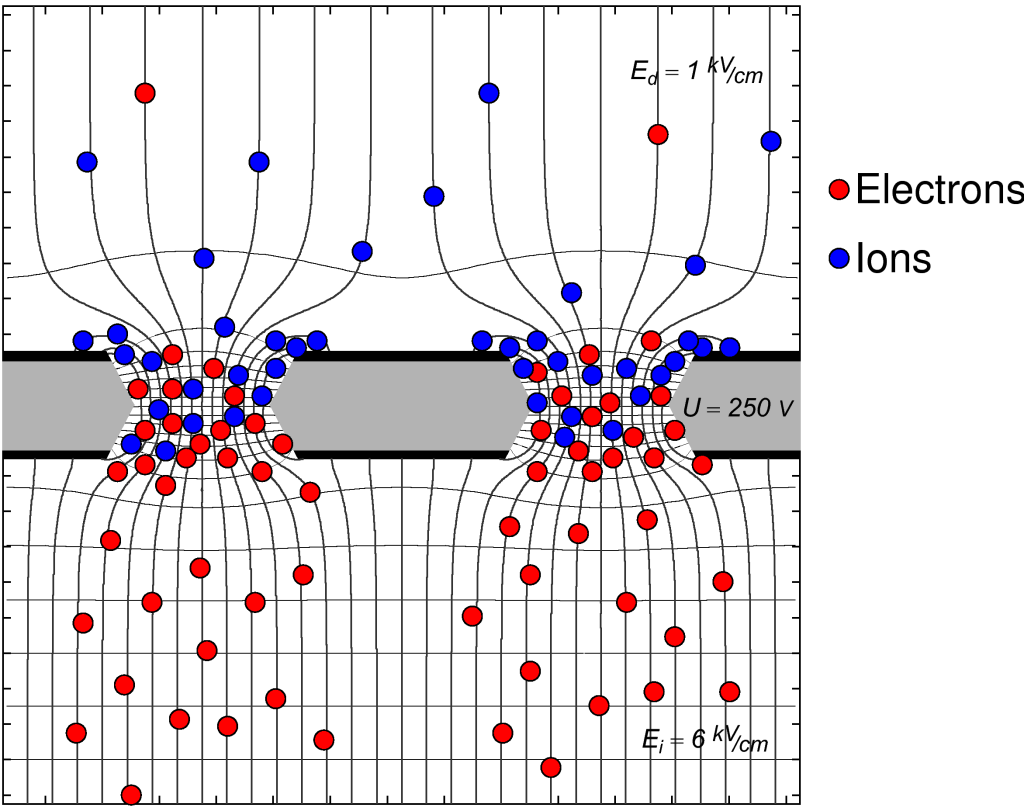
\includegraphics[width=\linewidth]{thesis_figures/GEM_field.png}

     \caption{A sketch of GEM field lines~\cite{GEM_field}.}
     \label{fig:GEM_field}
   \end{minipage}
   \hfill
   \begin{minipage}[t]{.45\textwidth}
     \centering
     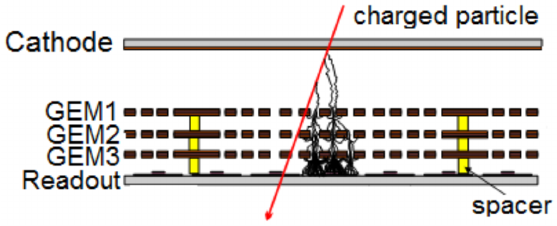
\includegraphics[width=\linewidth]{thesis_figures/GEM_process.png}
     \caption{Schematic of a triple GEM detector along with the working principle~\cite{article_GEM_pic}}
     \label{fig:Triple_GEM}
   \end{minipage}
 \end{figure}

\section{Track-Reconstruction Algorithm}

\subsection{Linear Regression}
\label{sec:Linear_Regression}
Linear regression for track fitting involves fitting a straight line to the data points, hits in our case with the condition that the total error is minimized. The total uncertainty is calculated as a sum of squares of individual measurement errors. Since the final result is dependent on minimizing the sum of the squares this approach to linear regression is known as least-squares approach. A simple mathematical description of the method is given below.

The equation of a straight line is given by $y=mx + c$, where $m$ is the slope of the line and $c$ is the intercept on the $y$ axis in a Cartesian coordinate system. The final goal is to obtain a good estimate for the two parameters $m$ and $c$. To obtain this estimate the square of error needs to be minimized. The error is the difference between the actual measurement $(x_i,y_i)$ and the prediction from our model, the equation of straight line. This error is also known as the residual and is defined as $r_i = y_i - m x_i - c $ for an $i^{th}$ measurement. Suppose that $n$ hits are measured then to obtain an estimate for $m$ and $c$ we need to minimize $\sum_{i=1}^n r_i^2$. The minimized estimates have the following values:
\begin{equation}
      \text{min}(m) = \frac{\sum_{i=1}^n x_i y-i - 1/n \sum_{i=1}^n x_i \sum_{i=1}^n y-i}{\sum_{i=1}^n x_i^2 - 1/n ()\sum_{i=1}^n x_i)^2}  = \frac{\bar{xy} - \bar{x}\bar{y}}{\bar{x^2-\bar{x}^2}}
\end{equation}
\begin{equation}
      \text{min}(c) = \bar{y} - \text{min}(m) \bar{x}
\end{equation}

A more detailed mathematical description can be found in \cite{Linear_regression}. The quality of the fit can be evaluated by calculating the reduced chi-square $\chi^2_{red}=\frac{\chi^2}{ndf.}=\frac{1}{ndf.}\sum_i \frac{(r_i)^2}{\sigma^2}$ where $\sigma$ is the resolution of each detector which might not be equal and ndf. are the number of degrees of freedom available for the fit.

Linear regression can also be used for NA64 to fit for the bending due to the magnets by replacing the model function from the equation of the straight line to some polynomial function. Such a method is called polynomial regression~\cite{STIGLER1974431}.

\begin{figure}[t!]
\centering
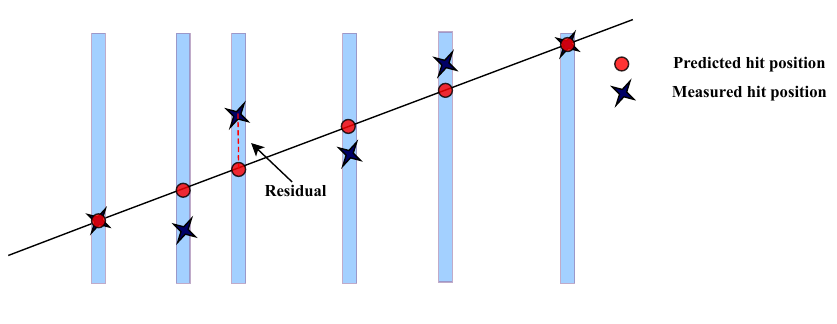
\includegraphics[width=\textwidth]{thesis_figures/linear_reg_new.png}
\caption{Linear regression pictorially. }
\label{fig:linear_regression}
\end{figure}

\begin{description}
  \item $\bullet$~\textbf{Filtering} is estimating the "present" state vector taking into account all the present and "past" measurements. Filtering from $m_1$ to $m_k$ includes filtering $m_1$ to $m_{k-1}$, then propagating from $m_{k-1}$ to $m_k$ and including $m_k$.
  \item $\bullet$~\textbf{Prediction} is estimating the state vector at a "future" time.
  \item $\bullet$~\textbf{Smoothing} is estimating the state vector at any point based on all the measurements.
\end{description}



%%% Local Variables:
%%% mode: latex
%%% TeX-master: "mythesis"
%%% End:

% !TEX root = mythesis.tex

%==============================================================================
\chapter{Detector exposure and Limits to the diffuse flux}
\label{sec:align}
%==============================================================================
 
The chapter aims to detail the procedure used to calculate the detector exposure or sensitivity to neutrinos for the DG$\mathrm{_{low}}$ region. The efficiencies calculated in the last chapter are used and the final expected neutrino rates are calculated. The first part of the chapter describes the exposure calculation along with the exposure contribution from different channels. Systematic uncertainties which can arise during the full analysis along with their contribution to the exposure are also discussed. 
The second part of the chapter details the results of the unblinding where no possible neutrino candidates were found for the angular range. Using this information an upper limit on the incoming flux of UHE $\nu$ is calculated. This limit is further compared to the one obtained by the previous analysis for the same time period but without the contribution of new triggers. The overall improvement forms a crucial result of this work. 


\section{Exposure Calculation}
\label{sec:det_exposure_calc}

One of the most accurate techniques used at Auger to calculate the exposure of the SD array to UHE$\nu$ is through extensive simulations of different detector configurations. In this method MC neutrino showers are thrown over varied detector configuration to calculate the effective or active area at each instant of time. Since the detector configuration of the SD array is constantly changing(\textit{faulty tanks, regular maintenance etc.}), sometimes on a daily basis, this technique requires a large amount of computational time and resources making it less desirable for use in this analysis. 

In this analysis, a different approach based on the 6T5 condition, which is required for each selected event in this analysis, is used for the exposure calculation. For this calculation, the 6T5 hexagon is taken to be the smallest possible detection unit for the $\nu$ event. The effective area i.e. the area seen by the incident cosmic neutrino for this detection unit at full efficiency is given by the Brillouin area~\cite{PierreAuger:2010zof}, $A_{6T5} = 1.95km^2$ as shown by the shaded area in fig~\ref{}. The aperture for this detector unit is dependent on the energy of the primary neutrino ,the slant depth in the atmosphere, X, neutrino flavor, type of the interaction, zenith angle, azimuth angel and the point of impact of the shower on the ground. The effective \textit{acceptance} of the detector unit can be written as follows:

\begin{equation}
  \label{eq:nu_accep}
  A_{hex}(E_{\nu}, X)  = \int^{\phi = 2\pi}_{\phi = 0} \,d\phi \int_{\theta_{min} = 58.5^{\circ}}^{\theta_{max}= 76.5^{\circ}}  \, A_{6T5} \cdot \varepsilon(E_{\nu}, X, \theta) \cdot sin\theta cos\theta \cdot d\theta    \mathrm{[cm^2 sr]}
\end{equation}

,where $\varepsilon(E_{\nu}, X, \theta)$ is the neutrino detection efficiency for each simulated energy, slant depth and zenith discussed in the last chapter. An example for a particular combination is given in fig.~\ref{}. Plots for efficiency for each combination can be found as part of the git code made available for this analysis. 

The next step involves integrating the \textit{acceptance} over the different simulated injected slant depths (as given in table~\ref{tab:Simulation_params}). This accounts for the \textit{effective mass} target for the neutrino identification over the 6T5 hexagon unit. It is calculated as follows. 

\begin{equation}
  \label{eq:nu_eff_mass}
  M_{hex}(E_{\nu}) = \int_X A_{hex}(E_{\nu}, X) \cdot dX
\end{equation}

Fig.~\ref{} shows the effective mass for both CC and NC interaction channels for a single 6T5 hexagon unit. Like the detection efficiency it increases with energy. 

Exposure calculation still needs to account for the detector configuration and its evolution over time. We reduced our array to units of 6T5 hexagons and a full SD array consisting of 1660 stations consists 1420 of these hexagons. Since the establishment of the Pierre Auger Observatory the active number of 6T5 hexagons are monitored every second. This forms a very good indicator for the time evolution of the SD array since any non-working station or large periods of instability are intrinsically recorded in the number of active 6T5 hexagons at that time. The instantaneous number of hexagons, $n_{hex}(t)$ thus can be used as an indicator of detector configurations over time. The $n_{hex}(t)$ were updated and calculated every minute and have an uncertainty of about 1.5\% as mentioned in~\cite{PierreAuger:2010zof}. To calculate the energy dependent exposure, the effective mass of one 6T5 hexagon is multiplied by the instantaneous number of hexagons and integrated in time. Further, the $\nu$ interaction probability for each flavour(i = $\nu_e, \nu_{\mu}, \nu_{\tau}$) and channel(c = CC, NC) is also folded in. The exposure is given as:

\begin{equation}
  \xi^{i,c}(E_{\nu}) = \frac{\sigma^{i,c}(E_{\nu})}{m_N} \int_{t} M_{hex}^{i,c}(E_{\nu}) \cdot n_{hex}(t) \cdot dt =  \frac{\sigma^{i,c}(E_{\nu})}{m_N} \cdot M_{hex}^{i,c}(E_{\nu}) \cdot N_{hex}
\end{equation}

,$\sigma^{i,c}(E_{\nu})$ is the neutrino nucleon cross-section~\cite{Cooper-Sarkar:2011jtt} and $N_{hex}$ is the total number of active 6T5 hexagons integrated in time over the search period. The value for $N_{hex}$ calculated for the period analysed is . The energy dependent exposure for different flavors and interaction channels is shown in fig~\ref{fig:Exp_flavors_comp}. It is necessary to point out again that the double bang showers which can be produced by $\nu_{tau}$ are not taken into account for this analysis which was also mentioned in sec.~\ref{sec:sim_DGL} 

\begin{figure}[t!]
  \centering
  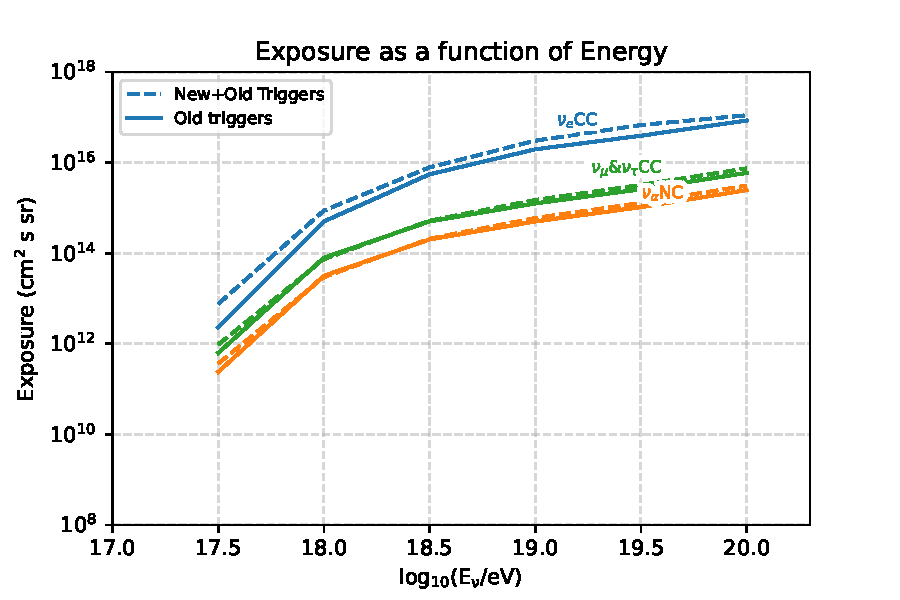
\includegraphics[width=14.5cm]{thesis_figures/ExpLimits/Exposure_comp_all_anotated_new_sim_optim.pdf}
  \caption{Exposure different channels}
  \label{fig:Exp_flavors_comp}
\end{figure}

An effective or total exposure, $\xi_{tot}(E_{\nu}) = \sum_{i}\sum_{c} \xi^{i,c}(E_{\nu})$ is calculated by summing all the interaction channels and assuming a 1:1:1 flavour ration at earth(large propagation distances combined with neutrino oscillations) as shown by the red line in fig~\ref{fig:Exp_total_comp}. 

\begin{figure}[t!]
  \centering
  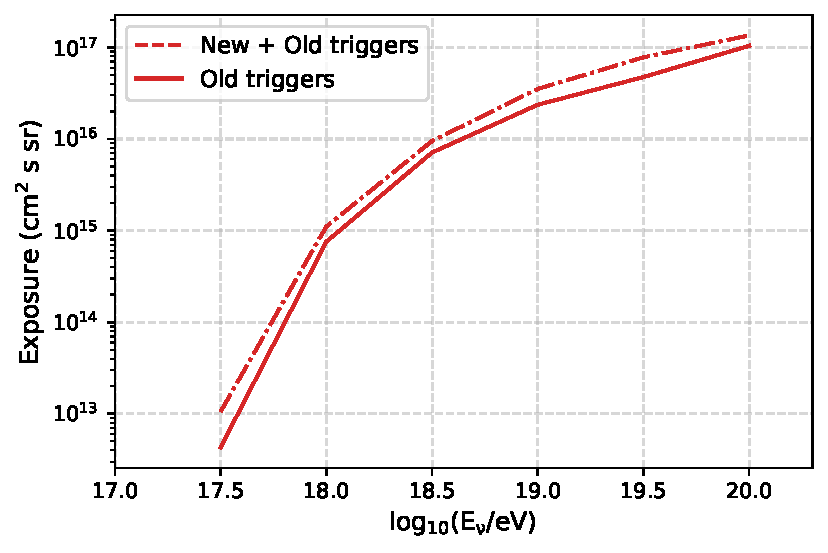
\includegraphics[width=14.5cm]{thesis_figures/ExpLimits/Exposure_comp_total_new_sim_optim.pdf}
  \caption{Total exposure}
  \label{fig:Exp_total_comp}
\end{figure}

As seen in the figure the $\nu_e$ CC channels contributes the most to the total neutrino exposure($\sim$85\%). The exposure rises rapidly at lower energies and then mostly flattens with just a slight increase which is due to the energy dependent neutrino cross-section. The shape is due to the neutrino detection efficiency which is small at lower energies as shown in fig~\ref{} in the last chapter. The next dominant channels are the $\nu_{\tau}$ and $\nu_{\mu}$ which have a similar detection efficiency as the NC channel but have a higher value of cross-section. The NC channel contribution is very small($\sim$5\%) due to the reasons discussed in section ~\ref{subsec:nu_sel_nudeteff}.  

The exposure calculated this analysis is compared to the one calculated using the previous analysis for the same time period in fig~\ref{fig:Exp_flavors_comp}. For the CC channel a 5x improvement is seen at lower energies and a 2x improvement at higher energies. For NC this improvement is not that significant. There is a 2x improvement at lower energies and a 1.5x improvement at higher energies. The improvement at lower energies is due to the inclusion of the new triggers MoPS and ToTd which enhance the detection efficiency at lower energies. The improvement at higher energies is mainly due to the improved Fisher analysis. The total exposure is also improved by a factor of ... 

\section{Systematic uncertainties}
\label{sec:det_uncert}
\todo{Determine what to write}
HERWIG PYTHIA difference take from old analysis.
PDF difference what is this ?
Hadronic interaction calculate yourself for 72 deg and $10^{19}$eV
https://scipost.org/SciPostPhysProc.13.028/pdf for CORSIKA vs others.
GAP2010-027 sytematic uncertainities neutrinos 
Also consider tau energy Loss maybe already mentioned in 2010 neutrino paper. 
Offline fluctuations and different reconstruction algorithms quote your own work.
can also quote An improved limit to the diffuse flux of ultra-high energy neutrinos
from the Pierre Auger Observatory(doi:10.1103/PhysRevD.91.092008) 
\section{Data unblinding}
\label{sec:data_unblinding}
As mentioned before in section~\ref{subsec:nu_sel_samp} the search data comprises of all events recorded at the Observatory between 2014-2021 which have a SD ID number non-divisible by 5 i.e. 80\% of all SD data recorded between 2014-2021. This search data sample was further split into a 20\% test sample similarly where SD ID numbers divisible by 4 were taken to be a part of the test sample while the rest became the part of the 60\% search sample. This split was done to perform the unblinding in two stages. The first where only the test sample in unblinded to detect any flaws with the analysis and if and when those flaws are fixed, the rest of the data is unblinded. This exercise turned out to be useful as a slight flaw was uncovered during the unblinding process of the 20\% test sample which was corrected. Said flaw which is described in more detail later required the whole reconstruction process along with the training of the Fisher polynomial to be performed again. This also led to the unblinded 20\% test sample to be blinded again since the reconstruction was altered. The splitting procedure was repeated and the total unblinding was performed again in parts. It is important to mention in all of unblinding procedure \textbf{0 neutrino events survive} the analysis selection.
This section is thus split into two subsections. The first describing the unblinding of the 20\% test sample along with the changes brought about by this unblinding. The second section details the full unblinding of the redone search samples (test + remaining) and discusses the interesting features of the unblinded search samples. 

\subsection{20\% test sample}
\label{subsec:unblind_20}

\todo{Test sample before the reco changes:}
% \begin{figure}[t!]
%   \centering
%   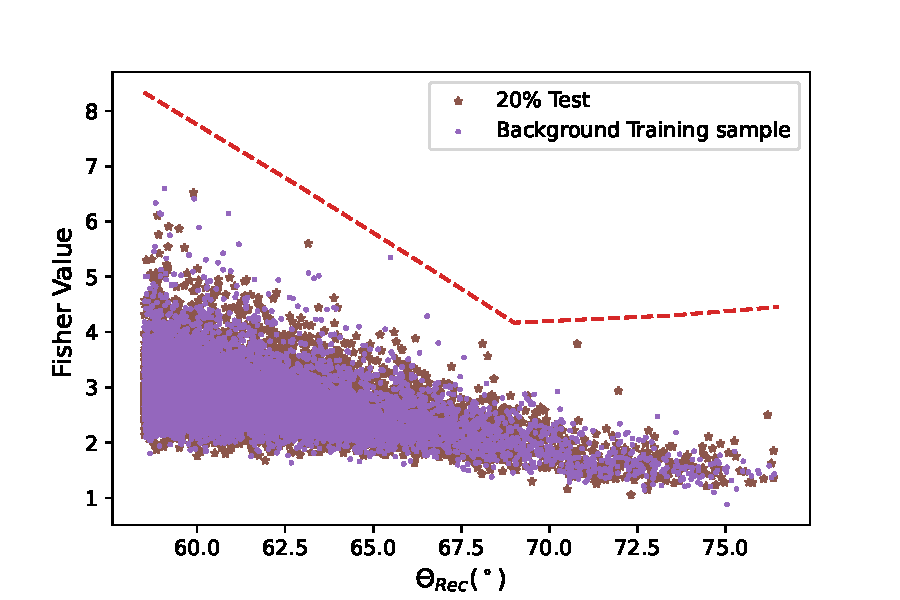
\includegraphics[width=14.5cm]{thesis_figures/Nu_analysis/Fisher_plots/Fisher_comp_bkg_test_wnt.pdf}
%   \caption{Test_reval vs background}
%   \label{fig:Fish_bkg_test}
% \end{figure}

The Fisher value distribution for the test sample is shown in fig~\ref{}. As it is shown no event passes the Fisher cut in any angular region. However, there are a few events which come very close to the cut line. Five events marked with a red circle were analysed in more detail. Each of them has its own unique reason with only the one with zenith~ being the most interesting. This event has the ID of 66106356. After looking at detailed information about the event it was found out that the accidental station cut used is insufficient. Previously, the  accidental cut (rejection of stations with Totalsignal < 3 VEM) is only applied to the event if there are more than 5 stations in the event. Since for this analysis due to the inclusion of MoPS and ToTd an overall increase in events is expected which also increases the overall number of stations with accidental stations this cut needs to be reduced a bit to take this overall increase into account. Thus, this cut was reduced to apply for events with more than 4 stations. This reduction of the cut decreases the total events passing the analysis cut by $\sim$5\% for the background training sample and $1-2$\% for the signal training sample. The Fisher coefficients and cut changes slightly. After this change in the reconstruction the test sample was obtained again and compared to the background dample as shown in fig~\ref{fig:Fish_bkg_test}. The other interesting events which have $\mathcal{F}$ values close to the $\mathcal{F_{cut}}$ with their respective ids are tabulated in table~\ref{}. These events were individually evaluated. Some of these () were found to have a bad time residual fit primarily because of multiple peaks observed in stations triggered by the new triggers. Since, no segmentation algorithm was used for stations with MoPS and ToTd triggers sometimes a wrong peak was selected which affected the reconstruction for these events. A future analysis with a corrected segmentation algorithm which is functional for the new triggers MoPS and ToTd is envisaged in the future analysis upgrades. Such events are expected to be limited to less than $\sim$1\% of total events but still require a careful look for future analysis upgrades. A further detailed analysis was also performed for these events where the primary mass composition was extracted via the muon production distributions as mentioned in~\cite{PierreAuger:2014zay}. Even with large uncertainties these events are most likely due to a light deep primary. For the other three events no particular feature worth mentioning was observed. 

\begin{figure}[t!]
  \centering
  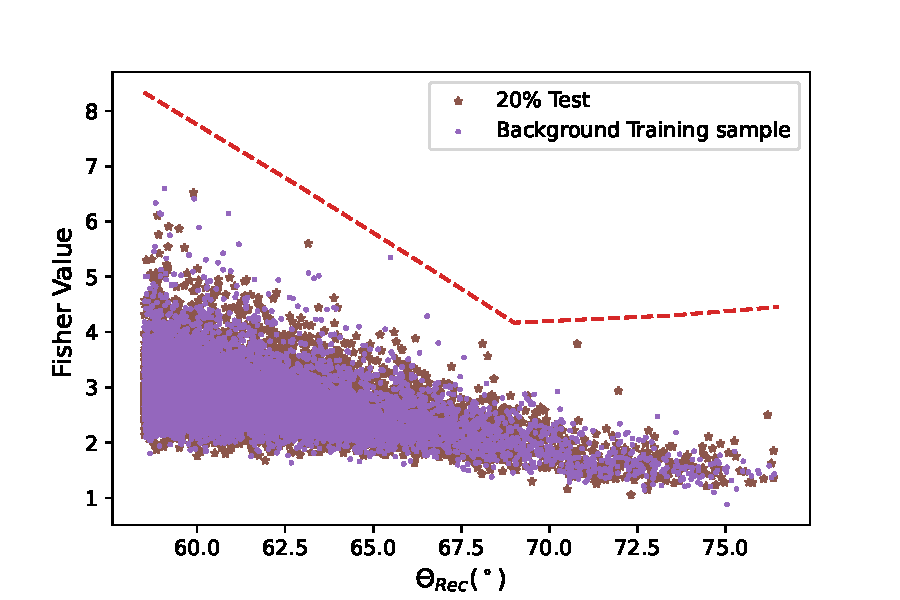
\includegraphics[width=14.5cm]{thesis_figures/Nu_analysis/Fisher_plots/Fisher_comp_bkg_test_wnt.pdf}
  \caption{Test_reval vs background}
  \label{fig:Fish_bkg_test}
\end{figure}

\begin{figure}[t!]
  \centering
  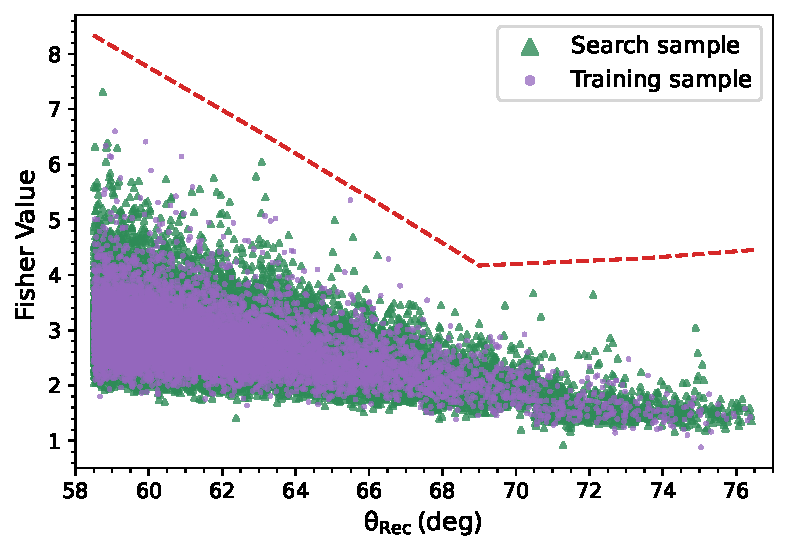
\includegraphics[width=14.5cm]{thesis_figures/Nu_analysis/Fisher_plots/Fisher_comp_bkg_search_wnt.pdf}
  \caption{Search vs background}
  \label{fig:Fish_bkg_test}
\end{figure}

\subsection{Reevaluated 20\% test search sample and 60\% search sample}
\label{subsec:unblind_60}
After the unblinding of the test sample and changing the cut mentioned in the section above, the unblinding was again performed in two stages. Initially a 20\% part was unblinded and then the remaining 60\% blinded sample was analysed. Again \textbf{0 neutrino candidates} were found after candidate selection. The results of the unblinding for each sub-angular bin is presented in fig~\ref{fig:Fisher_cut_2} along with the Fisher value as a function of zenith angle presented in fig~\ref{}. The results (red) are overlaid over the training(orange) and test (blue) samples with the dashed lines indicating the value of the $\mathcal{F_{cut}}$ obtained according to eq.~\ref{eq:fisher_poly_cut}. As it can be seen the distributions are compatible to each other within statistical fluctuations. The overlay also confirms that the exponential tail assumption is a reasonable enough to determine the $mathcal{F_{cut}}$. The goodness of the fit is once against presented in tab.~\ref{tab:Cut_eval_unblind} in the form similar to table~\ref{tab:Cut_eval}. This time for the observed values the numbers are calculated from the much larger search sample. It is found that the tails of the distributions which typically seemed to have fit badly also fit reasonably well. The events in the search sample that have $\mathcal{F}$ values close to the $\mathcal{F_{cut}}$ were again carefully checked and were found to be either due to the issues with the segmentation algorithm or known issues such as partial shower containment or large number of non-working PMTs both issues have also been seen in previous analysis. 

\begin{figure}[h!]
  \centering
   \begin{subfigure}[l]{.48\textwidth}
     \centering
     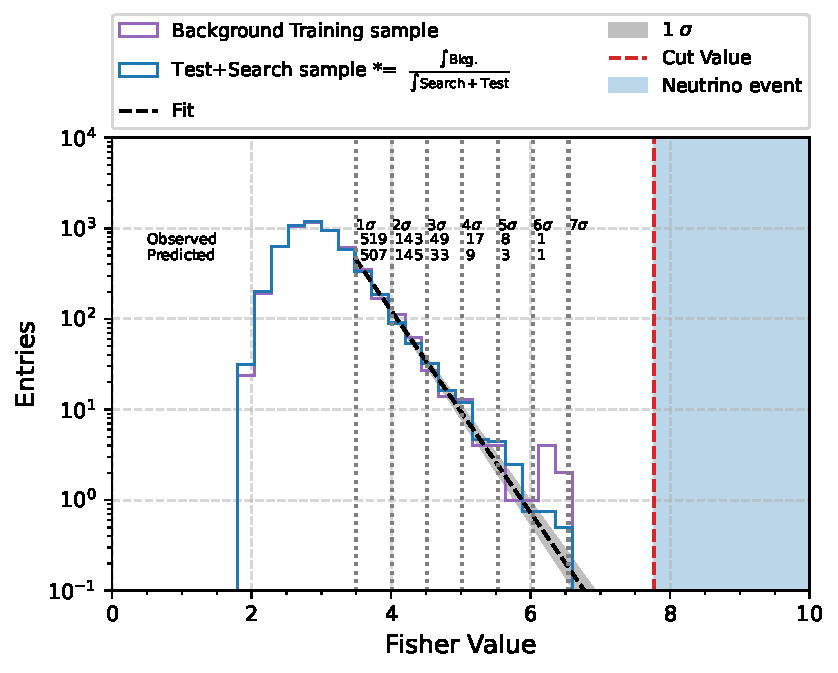
\includegraphics[width=\linewidth]{thesis_figures/Nu_analysis/Fisher_plots/Fisher_fit_search+test_bkg_region_58.5_61.5.pdf}
     \caption{58.5 61.5}
     \label{fig:58.5-61.5}
   \end{subfigure}
   %\hfill
   \begin{subfigure}[r]{.48\textwidth}
     \centering
     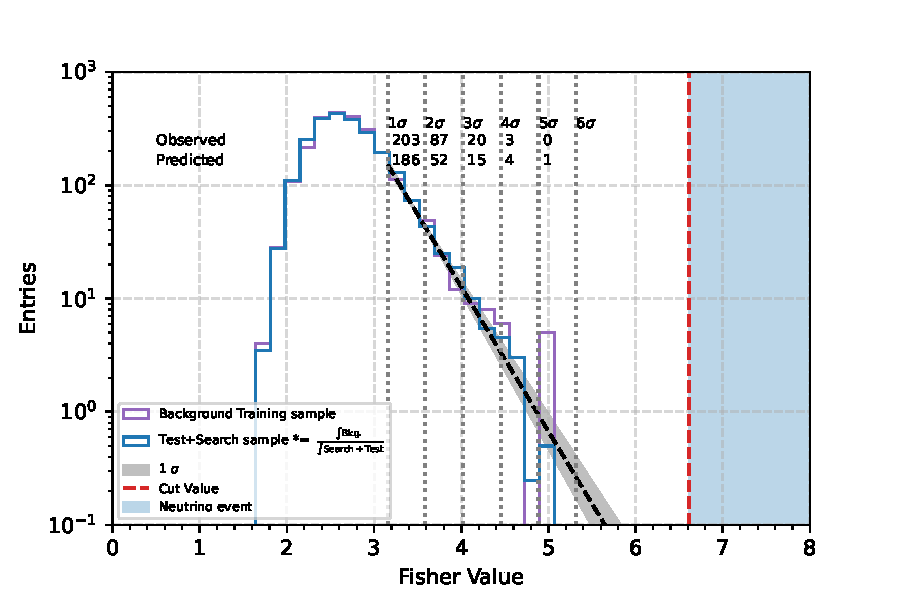
\includegraphics[width=\linewidth]{thesis_figures/Nu_analysis/Fisher_plots/Fisher_fit_search+test_bkg_region_61.5_64.5.pdf}
     \caption{61.5 64.5}
    \end{subfigure}
    \hfill
    \begin{subfigure}[l]{.48\textwidth}
      \centering
      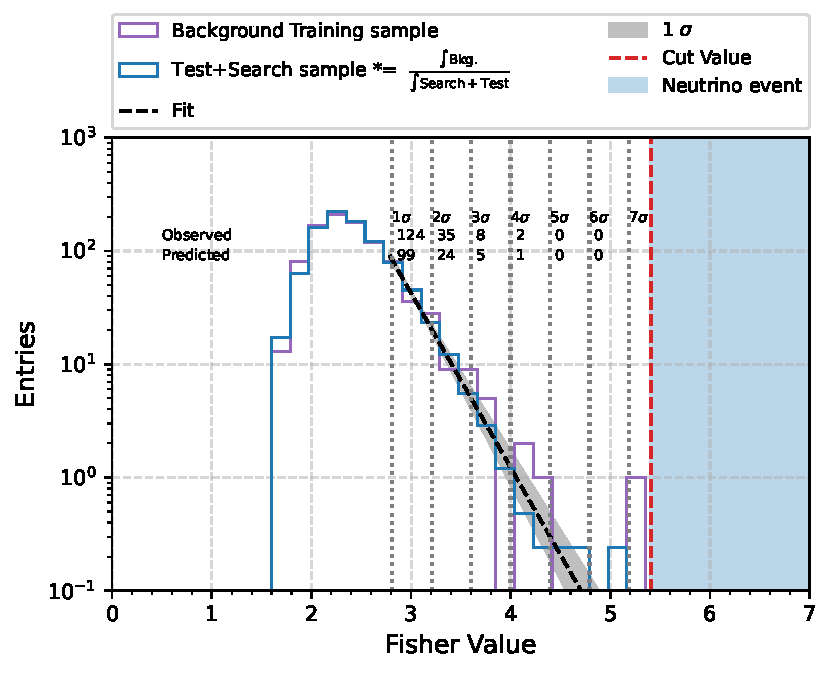
\includegraphics[width=\linewidth]{thesis_figures/Nu_analysis/Fisher_plots/Fisher_fit_search+test_bkg_region_64.5_67.5.pdf}
      \caption{64.5 67.5}
    \end{subfigure}

    \begin{subfigure}[r]{.48\textwidth}
      \centering
      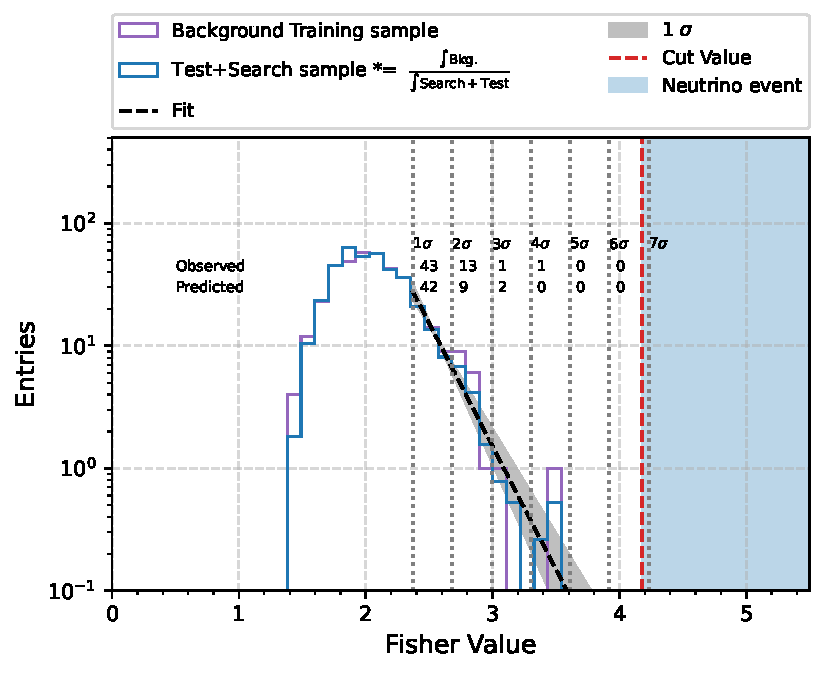
\includegraphics[width=\linewidth]{thesis_figures/Nu_analysis/Fisher_plots/Fisher_fit_search+test_bkg_region_67.5_70.5.pdf}
      \caption{67.5 70.5}
    \end{subfigure}
    \hfill    
    \begin{subfigure}[r]{.48\textwidth}
      \centering
      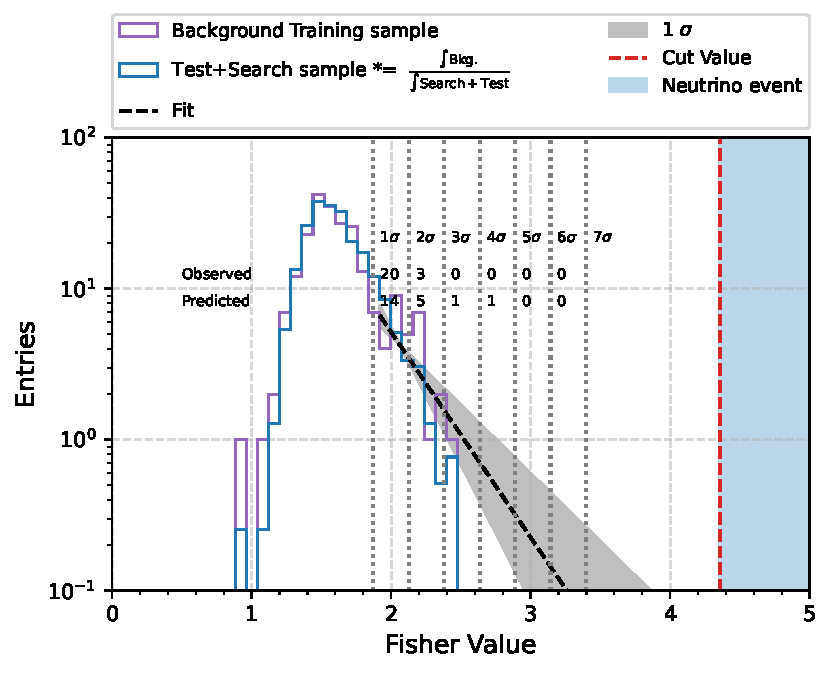
\includegraphics[width=\linewidth]{thesis_figures/Nu_analysis/Fisher_plots/Fisher_fit_search+test_bkg_region_70.5_73.5.pdf}
      \caption{70.5 76.5}
   \end{subfigure}
   \caption{Evaluating the goodness of fit of the Fisher cut for the search sample. The observed values are compared to the predicted values.}
    \label{fig:Fisher_cut_2}

\end{figure}

\begin{table}[h!]
  \centering
  \begin{tabular}{ |P{1.25cm}||P{2.4cm}|P{2.4cm}|P{2.4cm}|P{2.4cm}|P{2.4cm}| }
    \hline
      Fit & \multicolumn{5}{c|}{Number of events in $\mathcal{F}$ tails} \\
      Range & \multicolumn{5}{c|}{Observed - Predicted} \\
    \cline{2-6}
      & Region 1 & Region 2& Region 3& Region 4 & Region 5 \\
      &(58.5$^\circ$-61.5$^\circ$]&(61.5$^\circ$-64.5$^\circ$]&(64.5$^\circ$-67.5$^\circ$]& (67.5$^\circ$-70.5$^\circ$] & (70.5$^\circ$- 76.5$^\circ$] \\
    \hline 
    $\mu$ + 1$\sigma$ & 13 & 14 & 17 & 19 & 23 \\
    $\mu$ + 2$\sigma$ & 1640 & 1820 & 2040 & 2330 & 2720 \\
    $\mu$ + 3$\sigma$ & 140 & 220 & 140 & 230 & 120 \\
    $\mu$ + 4$\sigma$ & 140 & 220 & 140 & 230 & 120 \\
    $\mu$ + 5$\sigma$ & 140 & 220 & 140 & 230 & 120 \\
    $\mu$ + 6$\sigma$ & 140 & 220 & 140 & 230 & 120 \\
    \hline
  \end{tabular}
  \caption{Table to test captions and labels.}
  \label{tab:Cut_eval_unblind}
\end{table}
\section{Diffuse limit for the UHE neutrino flux}
\label{sec:diff_limit}
Since no neutrino candidate was found in this analysis, an upper limit to the flux of the incoming UHE$\nu_s$ can be evaluated. Let flux per unit area, \textit{A}, energy, solid angle $\omega$ and time be denoted by $\mathrm{\phi(E_{\nu}) = \frac{d^6 N_{\nu}}{dE_{\nu}d\omega dA dt}}$. The expected number of detected neutrinos can be calculated by folding in the total exposure $\xi_{tot}(E_{\nu})$ with flux as follows,

\begin{equation}
  \mathrm{N_{expected} = \int_{E_{\nu min}}^{E_{\nu max}} \phi(E_{\nu}) \cdot \xi_{tot}(E_{\nu}) \cdot dE_{\nu}}
\end{equation}

Assuming a differential UHE$\nu$ flux $\phi = k \cdot E_{\nu}^{-2}$, the integrated upper limit on the value of k is given by:

\begin{equation}
  \label{eq:integ_lim}
  \mathrm{k_{up} = \frac{N_{up}}{\int_{E_{\nu min}}^{E_{\nu max}} E_{\nu}^{-2} \cdot \xi_{tot}(E_{\nu}) \cdot dE_{\nu}}}
\end{equation}

, the value of $\mathrm{N_{up}}$ for a given confidence level can be determined based on the number of observed events and the number of expected background events. Different statistical methods can be used to obtain the value for $N_{up}$ based on the confidence interval. In the next sections some of these different statistical approaches are discussed in more detail. The Feldman and Cousins limit with an extension that incorporates the systematic uncertainties discussed above is chosen as a final estimate for $\mathrm{N_{up}}$.

\subsection{Feldman and Cousins limit}
\label{subsec:FandC}
Feldman-Cousins method~\cite{Feldman:1997qc} is a statistical technique used to construct confidence intervals, particularly for Poisson distributed data. This approach addressed the key shortcomings of traditional methods used to construct confidence intervals especially for cases where the number of observed events are low or zero. Traditional methods such as Gaussian approximation, which assumes that data follows a normal distribution which are used to calculate confidence intervals can often lead to incorrect interval particularly in rare event searches where the data is better described by a Poisson distribution. This can also lead to unphysical values e.g. negative value for rate of expected events. The Feldman-Cousins approach solves these problems by giving a unified method for constructing confidence intervals. The method ensures that the intervals are unbiased and do not favour one outcome over the other. It also ensures natural transition from two-sided intervals(where there is significant data) to one-sided upper limits(when there is little to no data). The method also respects physical constraints, such as non-negative value for expected event rates. It also provides intervals with more accurate coverage probabilities, reducing over-coverage issues common in other methods. 

The Feldman \& Cousins approach is implemented as a part of \textit{gammapy} in python~\cite{Gammapy:2023gvb} which was used  to get the interval for this analysis. The information was also verified with look-up tables in~\cite{Feldman:1997qc}. For a 90\% confidence interval, in case of zero signal and background events, the upper and lower limits are given as $N^{90\%}_{up} = 2.44$ and $N^{90\%}_{low} = 0$ respectively. If one signal event is seen with zero background then this interval shifts to [4.36,0.11]. It is important to note that both statistical and systematic uncertainties are not included for the intervals calculated in the Feldman \& Cousins method. 

\subsection{Rolke approach}
\label{subsec:Rolke}
The Feldman \& Cousins treatment is a frequentist method which requires the background source to be known precisely. Such a method can fail if the uncertainties are too high~\cite{Rolke:2000ij}. To solve this problem one can also use the Rolke method~\cite{Rolke:2004mj} which incorporates prior information in this case signal with a Poisson distribution and background with either a Poisson or Gaussian distribution. The method is implemented as a ROOT class under TRolke~\cite{TRolke_ROOT}. For a 90\% confidence interval in the case of zero signal and background events the interval is given as [2.21,0] assuming a Poisson distribution for both signal and background. As it is seen the interval is smaller in comparison to the Feldman \& Cousins approach. This can be explained much more clearly for the case where there is one signal event and no background where the Rolke interval is [3.65,0]. In this case according to the Feldman \& Cousins approach the event has to be a signal since the lower limit is > 0 but in the Rolke approach it is still possible that such an event in the signal region could be a background event i.e. in the Rolke approach the absence of background does not imply zero background, but it only means that the background is not too large. This is because background is treated as a Poisson number. Thus, the overall upper and lower limits in the Rolke approach are always smaller in comparison to the Feldman \& Cousins  method. 

\subsection{Conrad approach}
\label{subsec:Conrad}
The Conrad method for calculating confidence intervals allows the inclusion of systematic uncertainties in the evaluation. Using this approach the uncertainties in the background prediction, background detection and the signal detection efficiencies can be incorporated in the confidence interval calculation by integrating over the PDFs of these parameters~\cite{Conrad:2002kn}. The method computes the upper limit based on a likelihood ratio between the observed data and the null hypothesis(no signal). For this work the interval was calculated using POLE++~\cite{Conrad:2005zm} which is a C++ program that implements the Conrad method. The systematic uncertainty on exposure was estimated to be as [] as mentioned in section~\ref{sec:det_uncert}. Using a uniform PDF to characterise the exposure and a Gaussian assumption for background, for a 90\% confidence interval in the case of zero signal and background events the upper and lower limits are given as: 

\begin{equation}
  \label{eq:Conrad_lim}
  N^{90\%}_{up} = 2.39\\
  \, N^{90\%}_{low} = 0
\end{equation}

The interval is smaller in comparison to the Feldman \& Cousins method due to the uneven interval for the systematic uncertainty. For one signal event and zero background the interval changes to []. 

\subsection{Final calculation}
\label{subsec:final_lim}
After the determination of $N_{up}$ using the Conrad approach the equation~\ref{eq:integ_lim} can be solved to determine the upper limit to the diffused flux of UHE$\nu_s$. The integral goes from $E_min = 10^{17.5} $eV till $E_max = 10^{20.5} $eV which is the total energy range explored in the simulations. It is also important to note that the limit is only valid for a smaller energy window. The single flavour 90\% C.L. integrated limit is given by 
\begin{equation}
  \label{eq:final_lim}
  \mathrm{k_{90} < 6.3 x 10^{-17} GeV cm^{-2} s^{-1} sr^{-1}},
\end{equation}
It applies to an energy range of $E_{\nu} \epsilon [1.9 \times 10^{18} - 2.0 \times 10^{20}]$ which is the energy range for which $\sim$90\% total event rate is expected in the case of $E^{-2}_{nu}$ flux. The value along with the 90\% energy range is plotted as a solid line in fig~\ref{}.

\begin{figure}[t!]
  \centering
  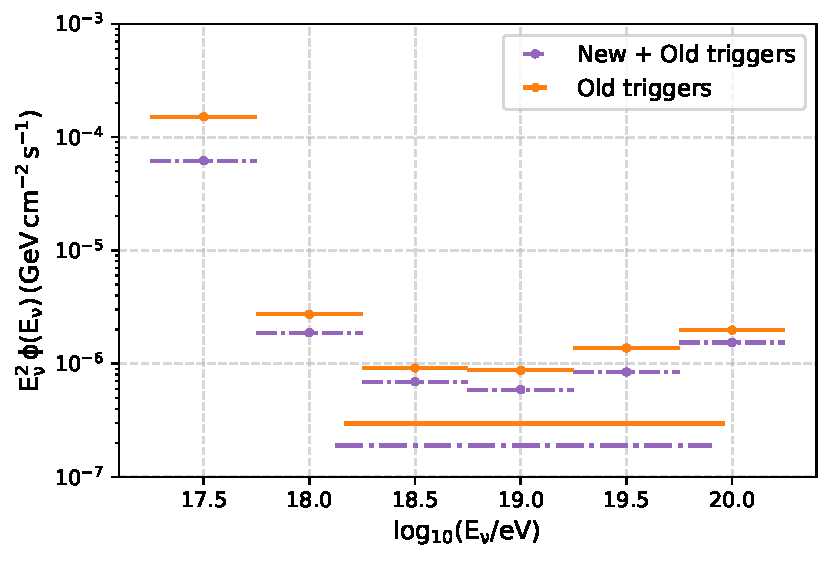
\includegraphics[width=14.5cm]{thesis_figures/ExpLimits/Integ_DiffLimit_comp_new_sim_optim.pdf}
  \caption{Diff limit new old comparison}
  \label{fig:Limit_comp_1}
\end{figure}

The other lines in green are the \textit{differential limits}. These are calculated by integrating the denominator of eq.~\ref{eq:integ_lim} in bins of width $\Delta = 0.5eV$ in $log_{10}(E_{\nu})$. Mathematically for the $i^{th}$ bin this can be represented as follows:

\begin{equation}
  \label{eq:diff_lim}
  \mathrm{Differential \,limit \, (i^{th} \, E_{\nu} \, bin)  = \frac{N_{Up}}{\int_{log_10(E^i - (\Delta log_{10}E)/2)}^{log_10(E^i + (\Delta log_{10}E)/2)} E^{-1}_{\nu} \cdot \xi(E_{\nu}) \cdot ln(10) \cdot d(log_{10}(E_{\nu}))}}
\end{equation}

Assuming constant exposure and flux in each energy bin the differential limit can be estimated as:

\begin{equation}
  \label{eq:diff_lim_approx}
  \mathrm{Approx. \, Differential \,limit \, (i^{th} \, E_{\nu} \, bin)  = \frac{N_{Up}}{E^{-1}_{\nu} \cdot \xi(E_{\nu}) \cdot ln(10) \cdot \Delta (log_{10}(E_{\nu}))}}
\end{equation}

These limits provide a way to denote the sensitivity of the detector for different energies. As it can be seen from the fig.~\ref{fig:Limit_comp_1} for the Down-going Low analysis the Pierre Auger Observatory is the most sensitive for energies $\sim$1 EeV. 

Both limits are also compared to the results from the previous analysis in fig~\ref{fig:Limit_comp_1}. As it was seen in the exposure comparison it is clear that the new triggers help improve the sensitivity at lower energies. For higher energies the improvements to the upper-limit for the diffuse flux of $UHE_{\nu_s}$ though not as signifivcant is still substantial. This improvement can be attributed to the changes in the Fisher analysis The integral flux limit sees an improvement $\sim$.. order of magnitude. The aim of this study was to evaluate the improvement, but it was always know that for this angular range significant improvements to the diffuse flux improvements were not expected. The diffuse flux limit and sensitivity for Auger is dominated by the Earth-skimming channel as shown in ~\cite{Aab_2019_diffuse}. This limit is significantly lower than the DG$\mathrm{_{low}}$ channel and is the main driver to constrain astrophysical and cosmogenic models. However, the improvements shown in this analysis are more important in the context of point source searches. This is discussed more in the next chapter. 

\begin{figure}[t!]
  \centering
  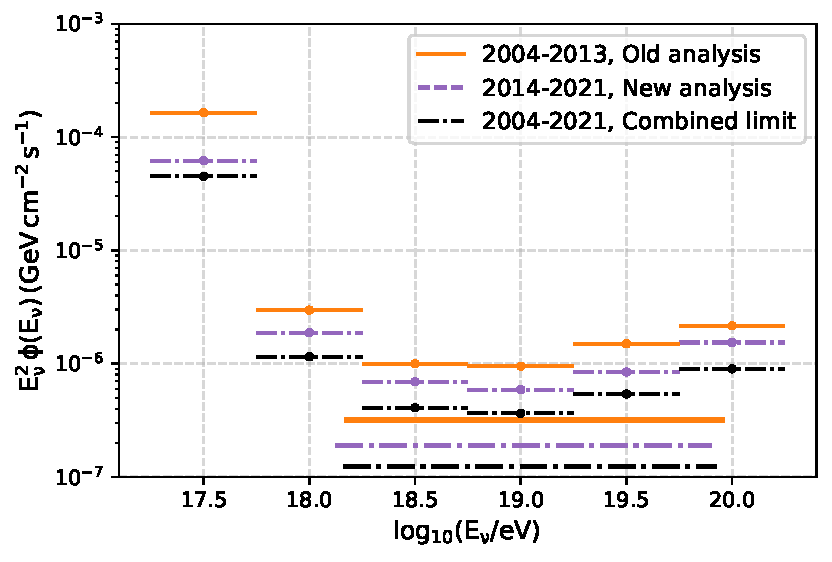
\includegraphics[width=14.5cm]{thesis_figures/ExpLimits/Integ_DiffLimit_comp_combined_new_sim_optim.pdf}
  \caption{Diff limit combination}
  \label{fig:Limit_comp_2}
\end{figure}

\begin{figure}[t!]
  \centering
  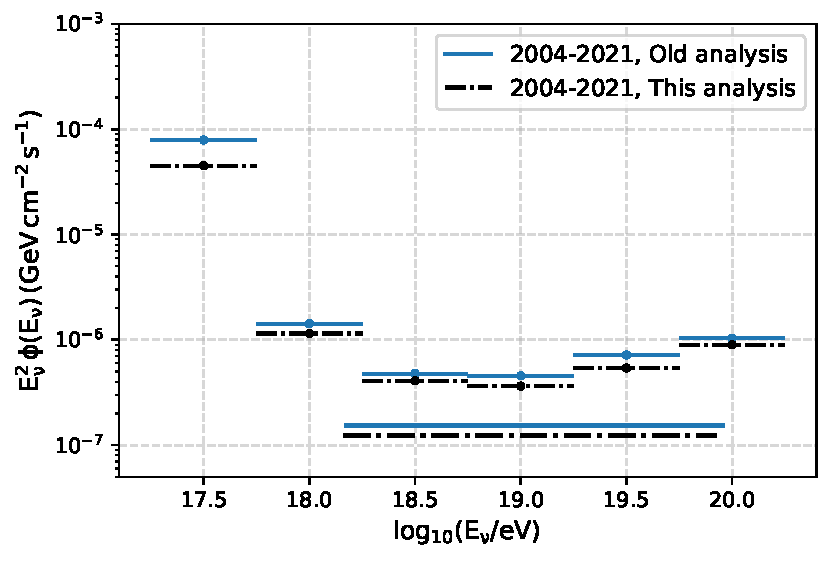
\includegraphics[width=14.5cm]{thesis_figures/ExpLimits/Integ_DiffLimit_comp_combined_new_sim_optim_3.pdf}
  \caption{Diff limit combination}
  \label{fig:Limit_comp_3}
\end{figure}


%%% Local Variables:
%%% mode: latex
%%% TeX-master: "mythesis"
%%% End:

% !TEX root = mythesis.tex

%==============================================================================
\chapter{Source follow-up analysis}
\label{chap:follow-up}
%==============================================================================

One of the most exciting fields of modern day neutrino astrophysics involves scanning the observable sky to look for neutrino sources. As mentioned in section~\ref{} the observation of TXS~\cite{} and NGC 1068~\cite{} which are examples of a transient source and a steady state of neutrinos has brought unprecedented excitement to the field. Any observation of a neutrino source offers a chance to significantly increase our overall knowledge about astroparticle physics. Since, Auger is one of the few experiments in the world sensitive to UHE$\nu_s$ any improvement in its point source sensitivity increases its capability for neutrino detection. 

In this chapter the point source sensitivity to $\nu$ events of the SD array is discussed for the zenith angular range explored in this thesis, DG$_{low}$. Based on the zero neutrino candidates found in the search performed in this work a source declination, $\delta$ dependent neutrino flux is calculated. This process includes calculating the declination dependent exposure and then converting it to a limit on the flux. The improvements to this exposure and sensitivity by the inclusion of new triggers is also discussed. Finally, the new limit is used to scan a few interesting sources which lie in the most sensitive range for the DG$_{low}$ region.

\section{Procedure for point source analysis}
\label{sec:procedure_point_source}

\subsection{Source visibility}
\label{subsec:psource_coverage}
The field of view of the Observatory and the corresponding neutrino efficiency is related to the zenith angle which in turn is related to declination. For a given point like source at declination $\delta$ and right ascension $\alpha$(in equatorial coordinates), the time zenith angle, $\theta$ dependence at a certain time, $t$ is given by:
\begin{equation}
  cos \theta(t) = sin \lambda \,sin \delta+ cos \lambda \, cos \delta \,sin (2\pi \frac{t}{T} - \alpha)
\end{equation} 
where $T$ is the duration of one sidereal day and $\lambda$ is the latitude of the observer($\lambda = -35.2^{\circ}$ for Auger). 
Fig.~\ref{} shows the FOV bands for different neutrino search channels(DGL, DGH, ES). These bands are plotted in equitorial coordinates as a function of $\alpha - t _{GS}$ where $t_{GS}$ is the Greenwich Sidereal Time(GST) converted to for a mean longitude of the Observatory, $l$ calculated as $t_{GS}= 2\pi t/T + l$. The sensitive declination ranges for different $t_{GS}$ can be read from the plot which is very useful for real-time transient follow-up. For DGL showers the SD of the Pierre AUger Observatory is sensitive to declinations between $\delta ~ -85^{\circ} - 40^{\circ}$. Another way to denote sky coverage for different neutrino searches at Auger is by calculating the time a source is visible to the Observatory for a particular declination. This is plotted in fig.~\ref{} for all three search channels. As it can be seen from the plot all three channels are the most sensitive at two ends of their sensitive declination ranges(DGL $\delta ~ -70^{\circ}, 35^{\circ}$) which is a consequence of smaller variation in zenith angle in time for certain directions. The sensitivity sharply decreases beyond these declination values. In the middle of these \textit{two horns} is a plateau like region. It is also seen that generally the fraction of time a source is visible is comparable in the DG$_{low}$ and DG$_{high}$ range with both being higher in the ES range due to the size of the zenith angle windows. The fraction of visible time for vertical showers is also plotted. Even though this fraction of time is significantly high no neutrino search can be performed for this region as it is very difficult to differentiate between a cosmic ray and neutrino shower for this zenith angle range. 

\subsection{Effective area and Exposure}
\label{subsec:psource_area}
Following this to calculate point source sensitivity, the declination dependent SD exposure is evaluated. This is done by first calculating an effective area to neutrinos of flavours i and energy $E_{\nu}$ is defined in the following way. For a point source spectral flux of flavour $i$ given by $\phi_i(E_{\nu}) = \frac{d^4 N_{\nu}}{dE_{\nu} dA dt}$ the expected number of detected events is given by 

\begin{equation}
  \frac{dN_{i}}{dt} = \int_{E_{\nu min}}^{E_{\nu max}} \, dE_{\nu} \, \phi(E_{\nu}) \, \mathcal{A}_i(E_{\nu})
\end{equation}
The effective area is flavour dependent since for each flavour the shower development and the primary interaction(c = NC, CC) is substantially different. The effective area is for the DGL region is given as follows:
\begin{equation}
  \mathcal{A_{i,c}}(E_{\nu},\theta(t),t) = \frac{\sigma^{i,c}(E_{\nu})}{m_N} \int_{X} \, \varepsilon_{i,c}(E_{\nu},\theta(t),t) A_{6T5} n_{hex}(t) dX
\end{equation}

where $\varepsilon_{i,c}$ is the neutrino identification efficiency for a 6T5 unit. The declination dependence is taken into account by the $\theta(t)$ dependence of the efficiency. The effective area for electron neutrinos with CC interactions in km$^2$ for 2016 array and different theta is plotted in fig.~\ref{}. The effective area increases with increasing primary energy. It also increases with zenith angles till ~70$^\circ$ after which there is a slight decrease in the effective area which is due to the decrease in neutrino sensitivity at higher zenith angles discussed earlier in section~\ref{}. 

The exposure to point-like sources of UHE neutrinos can then be calculated by integrating the effective area for a given time interval and summing over the different flavours and channels as follows:
\begin{equation}
  \xi(E_{nu}, \delta) = \sum_{i,c} \int_{t} \mathcal{A_{i,c}}(E_{\nu},\theta(t),t) dt
\end{equation}

The exposure is $\delta$ dependent due to the dependence of effective area on $\theta(t)$. The effective area can also change with time due to the changes in the number of hexagons $n_{hex}(t)$. This change has been visualized for the DG$_{low}$ channel for the time period of this search in fig.~\ref{}. As it can be seen in the plot the number is relatively stable especially in the period of one sidereal day apart from few outages which are removed from the searches. The directional exposure for the DGL channels for different fixed energies between 2014-2021 is shown in fig.~\ref{}. The solid line shows the exposure calculated in this study by including the new triggers while the dashed line shows the exposure calculated with the previous analysis for the same time period. Similar to the exposure calculated for the diffuse flux the exposure is significantly improved for lower energies with the improvement decreasing or vanishing for higher energies. The shape of the exposure is similar to the observation time plot in fig.~\ref{} with the maximum exposure peaks seen at the same declinations. ES exposure published in ~\cite{} is also plotted for comparison. It can be seen that generally the DG$_{low}$ point source exposure in lower than that of ES expect at higher energies where it is comparable. At these energies the different sensitive zenith angle ranges between the channels are the only differentiating factors for the exposure distribution. 

\section{Point-source neutrino flux limit}
\label{sec:pfux_limit}
Since no neutrino candidate was discovered in the search window a point-source neutrino flux limit can be calculated. Similar to the calculation for diffuse flux the number of expected neutrino events from a point like source at a given declination can be written as 
\begin{equation}
  N_{expected}(\delta) = \int_{E_{min}}^{E_{max}}  \phi(E_{\nu})  \xi(E_{\nu}, \delta) dE_{\nu}
\end{equation}
The point source flux is assumed to be independent of time and is assumed to be characterized as a power law, $\phi = k_{PS} E_{\nu}^{-2}$ for all declinations. The integrated upperlimit from each source can then be further calculated as follows:

\begin{equation}
  k_{PS}^{90\%CL} = \frac{N_{Up}}{\int_{E_{min}}^{E_{max}} E_{\nu}^{-2} \xi(E_{\nu}, \delta) dE_{\nu}}
\end{equation}

For this study initially a time period from 1 Jan 2014 till 31 December 2021 is selected. The N$_{Up}$ = 2.39 is calculated according to the Conrad approach as mentioned in section~\ref{}. The exposure is assumed to be uniform within $\pm 0.6\%$ for the time period of search as shown in ~\cite{}. 

The 90\% C.L. declination dependent upper-limit for the DG$_{low}$ channel is shown in fig.~\ref{}. The limit is the stringent for the times the source is seen the longest. The limit is calculated for the energy range ~ 2.0 $\times 10^{18}$eV - $\times 10^{20}$eV. The dependence of energy intervals is minimal. This limit is also compared to the limit obtained from the previous analysis for the same time period in fig.~\ref{}. As it can be seen the limit is significantly improved with new triggers fulfilling one of the primary objectives of this thesis.     
A cross-check of the diffuse limit is obtained from the point source analysis by performing double integration of the exposure, $\xi(E_{\nu}, \delta)$ in a similar way as done in~\cite{}.

The diffuse limit can be written as:
\begin{equation}
  k_{PS}^{90\%CL} < \frac{N_{Up}}{\int_{log_{10}E_{min}}^{log_{10}E_{max}} \int_{-\pi/2}^{\pi/2}2\pi \cdot cos(\delta) \cdot E_{\nu}^{-1} \cdot \xi(E_{\nu}, \delta) \cdot ln(10) \cdot d(log_{10}(E_{\nu})) \cdot d\delta} 
\end{equation}

The diffuse limit from point source analysis is given as: 
\begin{equation}
  k_{PS}^{90\%CL} < 2.0000 \times 10^{-8} GeV cm^{-2} s^{-1} sr^{-1}
\end{equation}

Which agrees with the value mentioned in eq.~\ref{}. It is also important to mention that even though the overall sensitive declination range for the DG$_{low}$ analysis is small in comparison to other channels~\cite{}, the improvement presented in this thesis is still important as the sensitive declination ranges are not fully overlapping. Thus, if there is a point source at between declinations $-80^{\circ}- -68^{\circ}$ then DG$_{low}$ channel offers the only window at Auger to see UHE$\nu_s$ from such a source.  




%%% Local Variables:
%%% mode: latex
%%% TeX-master: "mythesis"
%%% End:

% !TEX root = mythesis.tex

%==============================================================================
\chapter{Conclusion and Outlook}
\label{chap:conc}
%==============================================================================
% \begin{figure}[h!]
% \centering
% 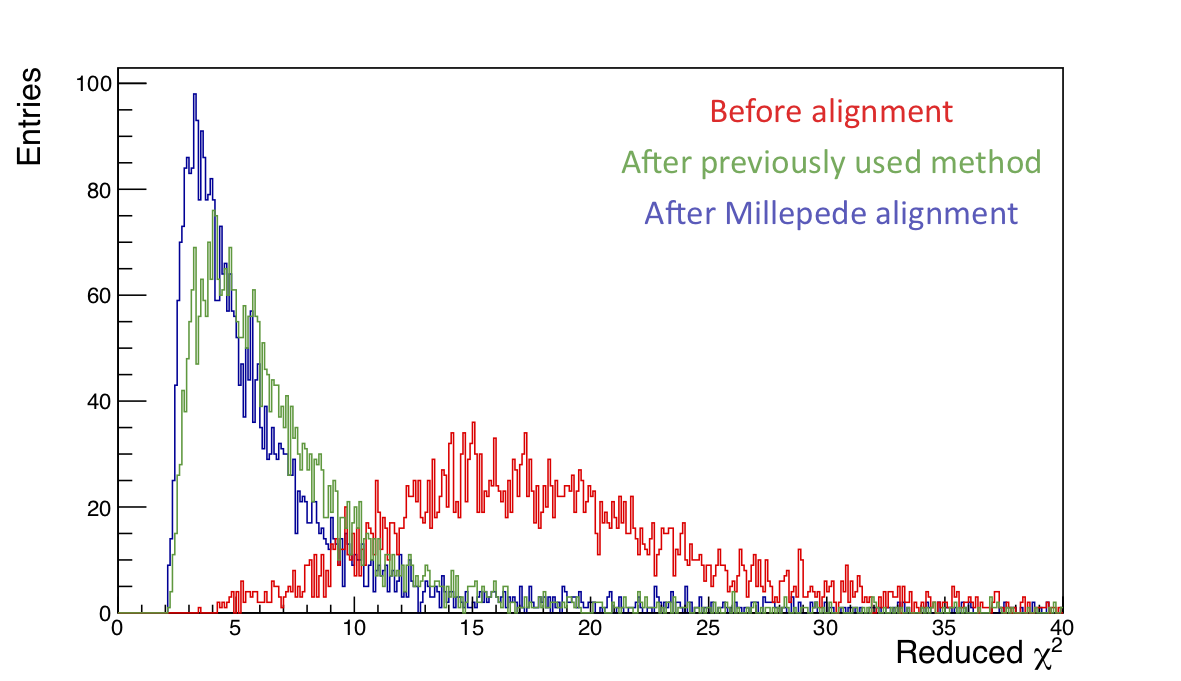
\includegraphics[width=0.85\textwidth]{thesis_figures/chi2_comp_conclusion_2.png}
% \caption{$\chi^2_{red}$ distribution for selected tracks showing the impact of Millepede alignment.}
% \label{fig:red_chi2_4}
% \end{figure}

Besides detecting ultra-high-energy (UHE) cosmic rays, the Pierre Auger Observatory with its large Surface Detector (SD) array offers a remarkable exposure to neutrinos above $10^{17}$eV. Any potential observation of such UHE$\nu_s$ will further our knowledge about the known universe. Since neutrinos are not deflected as they travel towards us at Earth, they offer a direct line of sight to the sources where they were produced. They are also some of the earliest particles produced in a transient source which makes their detection an important beacon for other astronomical instruments to perform a multi-messenger observation. The Pierre Auger Observatory is constantly monitoring the sky for the presence of such UHE$\nu_s$. The idea behind the detection remains the same as previous analysis at Auger where the neutrinos are assumed to induce Extensive Air Showers (EASs) close to the ground with a large electro-magnetic component at ground ("young" showers). This strategy is only employed for horizontal showers ($\theta > 60^{\circ}$). Two new SD triggers, time-over-threshold-deconvolved (ToTd) and multiplicity of positive steps (MoPS) were installed in 2014 to further increase the detection efficiency for low energy neutrino induced EASs. This thesis presents the first analysis of this improved efficiency for low energy neutrino showers in the zenith range $\theta \in [60^{\circ},75^\circ]$ also known as Down-going low or DG$_{Low}$ range. In this thesis the effect of the new triggers was evaluated for two types of searches, the searches for the diffused flux of UHE$\nu_s$ and search for point-like sources of UHE$\nu_s$. For both searches an overall improvement of efficiency is observed when information from the new triggers is incorporated in the analysis. A short summary of the three main contributions of this thesis along with an outlook detailing potential improvements are detailed in the next sections. 
\section*{Incorporating new triggers in the DG$\mathrm{_{low}}$ UHE$\nu_s$ searches}
During this thesis each facet of the DG$_{low}$ analysis was analysed. An effort was made to maximize the potential of the analysis. A blind search strategy similar to~\cite{gap_note_2013,Aab_2019_diffuse} was followed to avoid any bias in the analysis. The first step in this process was to include the information from the new triggers in the neutrino searches. About $\sim$7 years of recorded data was available for this task. The effect of the new triggers was first evaluated on neutrino simulations by including them in the analysis chain as described in section~\ref{subsubsec:nu_sel_fisher_training}. By the inclusion of new triggers an overall increase in reconstructed events was observed as shown in fig~\ref{fig:Events_vs_angle_summary}. This increase was most significant for lower energy neutrinos and decreased with increase in primary energy. This was an expected consequence due to the design of the new triggers. The overall increase also allowed for further modifications to the analysis which included lowering some stringent cuts as described in section~\ref{subsec:nu_sel_nudeteff}. For the final step of the analysis a Fisher discriminate polynomial was built and trained using the simulations (signal training sample) and a small fraction of recorded data, $\sim$20\% from the Observatory (background training sample). The polynomial is built with Area over Peaks (AoPs) of the stations and a differentiation between the background and signal is performed based on a cut on the Fisher value as given in eq.~\ref{eq:fisher_poly_cut}.
After the fixing the selection, a test sample was unblinded to catch any remaining flaws in the analysis. This proved worthwhile as a small error in the reconstruction was discovered during this process. The error was promptly corrected, and the whole selection procedure was re-evaluated, and the Fisher was retrained. Since the correction involved a change to the reconstruction procedure the blind search was redone from the start. After this correction the unblinding was again performed in two stages. The new test sample and the full blinded sample, 20\% + 60\% of recorded data between the period of 1 Jan 2014 to 31 December 2012 was analysed to search for neutrinos. \textbf{No neutrino candidates} were found in the search performed using the analysis described in this thesis. 

\subsection*{Outlook}
Even though a concerted effort was made to maximize the potential of the analysis presented in this thesis certain improvements could not be implemented and are thus summarized here for future studies. The segmentation algorithm used for reconstruction of events for neutrino searches was found to be not properly tuned for the new triggers, ToTd and MoPS. Thus, for this analysis the new triggers were completely removed from the segmentation algorithm. The primary purpose of the segmentation algorithm is to evaluate the correct start times for the WCD signals to decrease the effect of accidental muons which in turn affects the zenith angle estimation. A better tuned segmentation algorithm could thus further improve the neutrino search with new triggers. A more detailed summary of this topic along with examples of events where the segmentation algorithm fails and where it could help are presented in Appendix~\ref{sec:app_3}. This tuning could not be explored in this thesis but could be implemented in the future. Further, as seen in this analysis the angular reconstruction used for neutrinos is not particularly calibrated for EASs which originate deep in the atmosphere. This could also be rectified for the future to improve this analysis. Other techniques which involved computing the zenith angle via measuring the footprint of the shower cannot not be applied here due to the compact nature of EASs expected for the angular range explored. In this thesis a cut on the saturated and active PMTs was also explored but not implemented in the final analysis. A detailed study on such a cut could also be useful to increase the efficiency of the analysis. 

Further, work was done in this thesis to adapt the DG$_{high}$ analysis to the current $\mathrm{\overline{Off} \underline{line}}$ version which is detailed in Appendix~\ref{sec:app_4}. This work is still in progress and could be used in the future to evaluate and test potential improvements to the analysis. The impact of inclusion of new triggers for such an analysis is expected to be minimal due to their decreasing efficiency with increasing zenith angle. However, new triggers could still potentially improve the efficiency for neutrinos (E $\sim 10^{17}-10^{17.5}$eV) even in this angular range. 

\section*{Improvements to the diffuse flux limit for UHE$\nu_s$ with new triggers}
With no neutrino candidate detected a 90\% C.L. upper limit on the diffuse flux of UHE$\nu_s$ for the DG$\mathrm{_{low}}$ channel was evaluated. The limit was evaluated under the assumption of a diffuse flux given by $\mathrm{\phi \propto E_{\nu}^-2}$ with a 1:1:1 neutrino flavour ratio at earth. The integrated limit is given as:
\begin{equation}
    k_{90} < 1.9 x 10^{-17} \mathrm{GeV cm^{-2} s^{-1} sr^{-1}},
\end{equation}
in the energy range $E_{\nu} \in [1.3 \times 10^{18} - 2.5 \times 10^{19.5}]$eV. The integrated limit represents the value of the normalisation of the differential flux needed to predict $\sim$2.39 expected events. The number 2.39 was evaluated using a semi Bayesian extension of the Feldman \& Cousins treatment accounting for systematic uncertainties on exposure~\cite{Conrad:2002kn}. This limit is $\sim 40\%$ stricter than the one obtained without the new triggers for the same time period. Even though this improvement is significant 
\section*{Improvements to the point source searches for UHE$\nu_s$ with new triggers}
Further a point sensitivity comparison was also performed to evaluate the performance of the new triggers. The methodology was adopted from ~\cite{Aab_2019_point} and an energy and declination dependent exposure was evaluated for the DG$\mathrm{_{_low}}$ range. Using the no neutrino candidate detection ansatz, a 90\% C.L. upper limit on the neutrino flux from point-like sources as a function of source declination, $\delta$ was evaluated and presented in fig.~\ref{fig:Dec_limit_new old}. This limit was also shown to improve with the inclusion of new triggers. The improvement though small has an impact in the overall sensitivity since the different searches (DG$_low$, DG$_high$, ES) have different FOVs. It must also be stressed that Auger is one of the constantly running experiments sensitive to Energy ranges > $10^{18}$eV thus any improvement to its sensitivity is an important step for the potential future detection of UHE$\nu_s$.



%%% Local Variables:
%%% mode: latex
%%% TeX-master: "mythesis"
%%% End:

% Uncomment the following command to get references per chapter.
% Put it inside the file or change \include to \input if you do not want the references
% on a separate page
% \printbibliography[heading=subbibliography]

%------------------------------------------------------------------------------
% Use biblatex for the bibliography
% Add bibliography to Table of Contents
% Comment out this command if your references are printed for each chapter.
% \printbibliography[heading=bibintoc]

%------------------------------------------------------------------------------
% Include the following lines and comment out \printbibliography if
% you use BiBTeX for the bibliography.
% If you use biblatex package the files should be specified in the preamble.
\KOMAoptions{toc=bibliography}
{\raggedright
  \bibliographystyle{../refs/atlasBibStyleWithTitle.bst}
  % \bibliographystyle{unsrt}
  \bibliography{./thesis_refs,../refs/standard_refs-bibtex}
}

%------------------------------------------------------------------------------
\appendix
\part*{Appendix}
% Add your appendices here - don't forget to also add them to \includeonly above
%------------------------------------------------------------------------------
\chapter{Alignment Figures}
\label{sec:app_1}
%------------------------------------------------------------------------------
This appendix includes the comparison of residuals obtained from alignment using the previously used method and Millepede. The reduced chi-square comparison plots for the two methods were shown earlier.
It also includes the residual versus position plots for the Micromega detectors.
\begin{figure}[h!]
\centering
 \begin{subfigure}[l]{.45\textwidth}
   \centering
   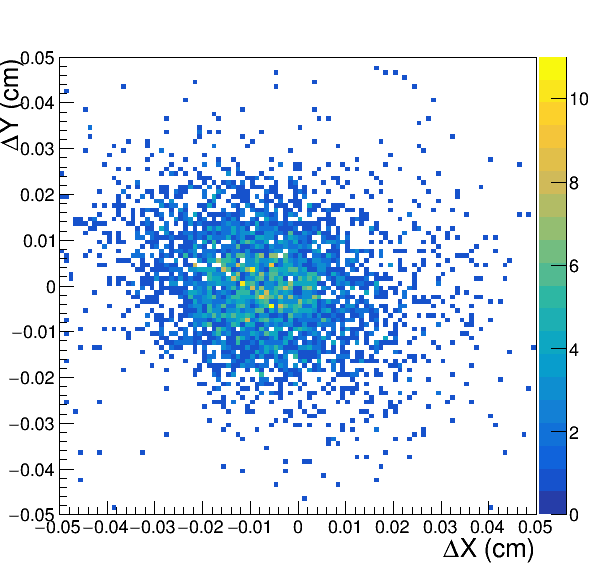
\includegraphics[width=\linewidth]{thesis_figures/alignment/Run_3211_after_prev/square/GEM1.png}

   \caption{GEM1 after previously used method}
   \label{fig:GEM1_after_prev}
 \end{subfigure}
 %\hfill
 \begin{subfigure}[r]{.45\textwidth}
   \centering
   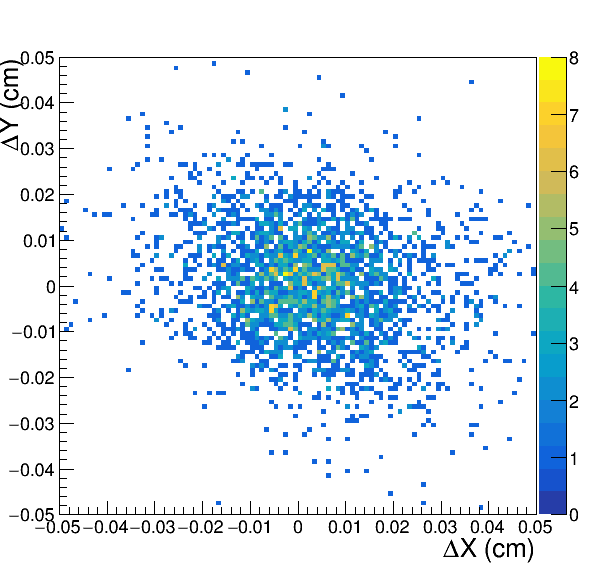
\includegraphics[width=\linewidth]{thesis_figures/alignment/Run_3211_after_millepede/square/GEM1.png}
   \caption{GEM1 after Millepede}
   %\label{fig:GEM1_before}
 \end{subfigure}
 \hfill
 \begin{subfigure}[l]{.45\textwidth}
   \centering
   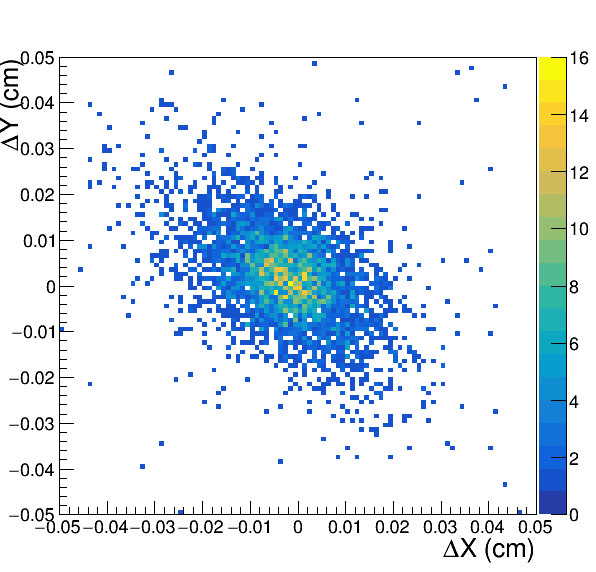
\includegraphics[width=\linewidth]{thesis_figures/alignment/Run_3211_after_prev/square/GEM2.png}
   \caption{GEM2 after previously used method}
   \label{fig:GEM2_after_prev}
 \end{subfigure}
 %\hfill
 \begin{subfigure}[r]{.45\textwidth}
   \centering
   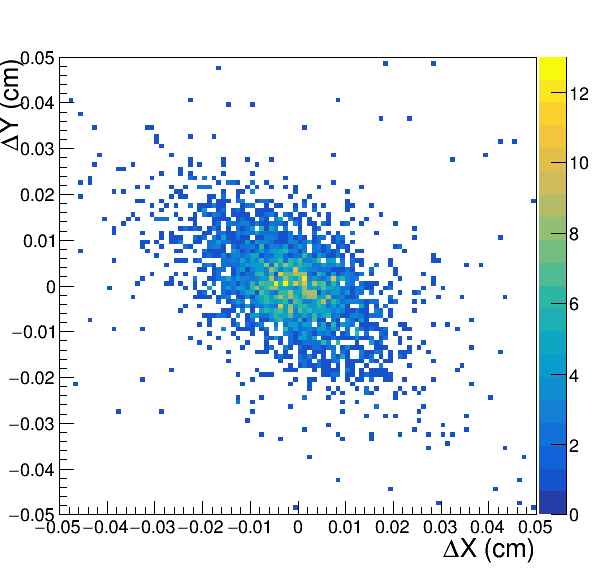
\includegraphics[width=\linewidth]{thesis_figures/alignment/Run_3211_after_millepede/square/GEM2.png}
   \caption{GEM2 after Millepede}
   %\label{fig:GEM2_before}
 \end{subfigure}
 \begin{subfigure}[l]{.45\textwidth}
   \centering
   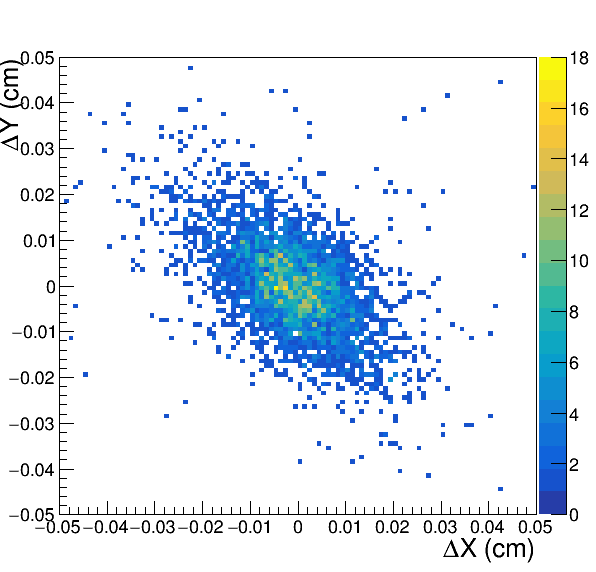
\includegraphics[width=\linewidth]{thesis_figures/alignment/Run_3211_after_prev/square/GEM4.png}

   \caption{GEM4 after previously used method}
   \label{fig:GEM4_after_prev}
 \end{subfigure}
 %\hfill
 \begin{subfigure}[r]{.45\textwidth}
   \centering
   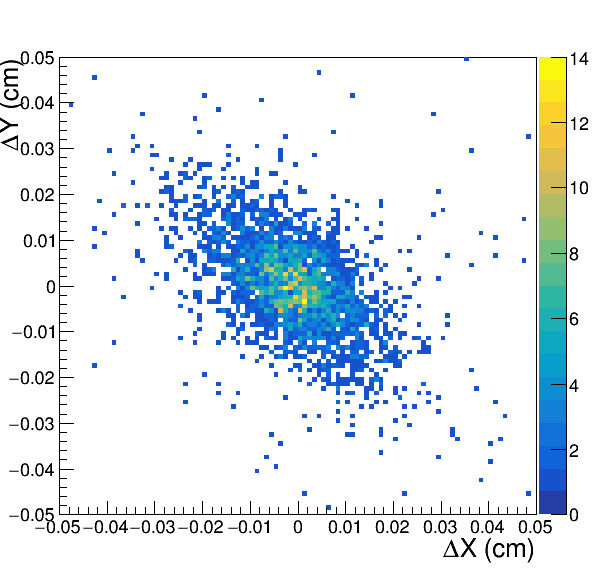
\includegraphics[width=\linewidth]{thesis_figures/alignment/Run_3211_after_millepede/square/GEM4.png}
   \caption{GEM4 after Millepede}
   %\label{fig:GEM4_before}
 \end{subfigure}
 \caption{Residual of GEM detectors.}
\end{figure}

%%%%MICROMEGAS start here

\begin{figure}[h!]
\centering
 \begin{subfigure}[l]{.45\textwidth}
   \centering
   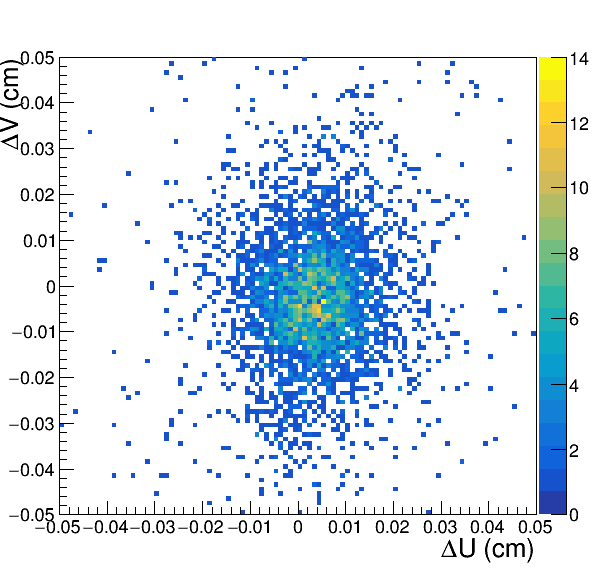
\includegraphics[width=\linewidth]{thesis_figures/alignment/Run_3211_after_prev/square/MX1.png}

   \caption{MM1 after previously used method}
   \label{fig:MX1_after_prev}
 \end{subfigure}
 %\hfill
 \begin{subfigure}[r]{.45\textwidth}
   \centering
   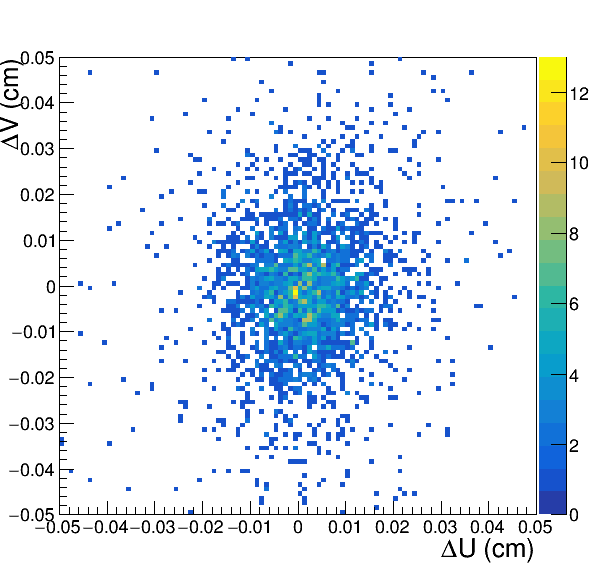
\includegraphics[width=\linewidth]{thesis_figures/alignment/Run_3211_after_millepede/square/MX1.png}
   \caption{MM1 after Millepede}
   %\label{fig:MX1_after}
 \end{subfigure}
 \hfill
 \begin{subfigure}[l]{.45\textwidth}
   \centering
   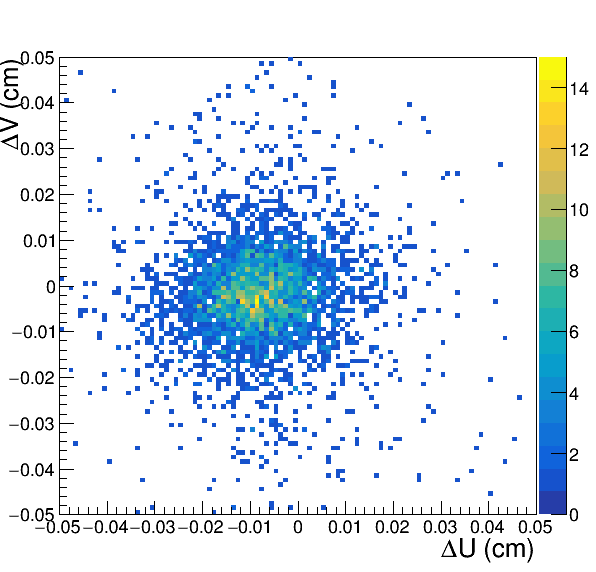
\includegraphics[width=\linewidth]{thesis_figures/alignment/Run_3211_after_prev/square/MX2.png}
   \caption{MM2 after previously used method}
   \label{fig:MX2_after_prev}
 \end{subfigure}
 %\hfill
 \begin{subfigure}[r]{.45\textwidth}
   \centering
   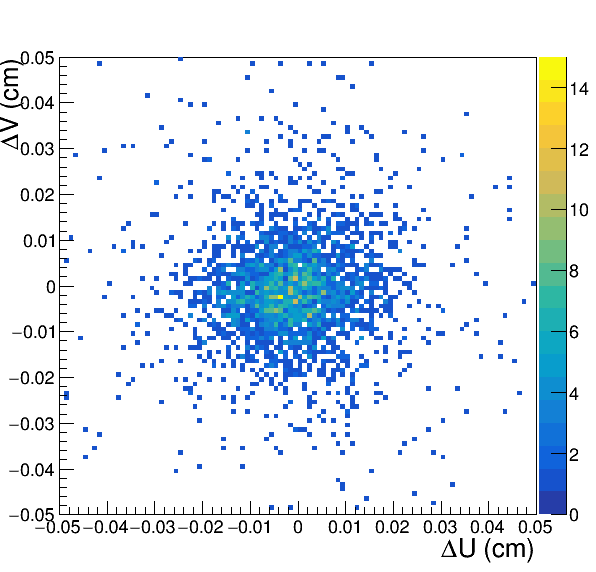
\includegraphics[width=\linewidth]{thesis_figures/alignment/Run_3211_after_millepede/square/MX2.png}
   \caption{MM2 after Millepede}
   %\label{fig:MX2_after}
 \end{subfigure}
 \begin{subfigure}[l]{.45\textwidth}
   \centering
   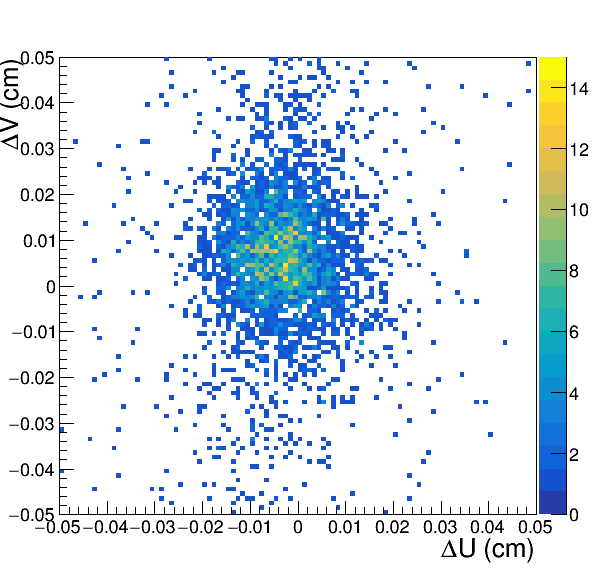
\includegraphics[width=\linewidth]{thesis_figures/alignment/Run_3211_after_prev/square/MX3.png}

   \caption{MM3 after previously used method}
   \label{fig:MX3_after_prev}
 \end{subfigure}
 %\hfill
 \begin{subfigure}[r]{.45\textwidth}
   \centering
   \includegraphics[width=\linewidth]{thesis_figures/alignment/Run_3211_after_millepede/square/MX3.png}
   \caption{MM3 after Millepede}
   %\label{fig:MX3_after}
 \end{subfigure}
 \caption{Residual of Micromega detectors.}
\end{figure}


\begin{figure}[h!]
\centering
 \begin{subfigure}[l]{.45\textwidth}
   \centering
   \includegraphics[width=\linewidth]{thesis_figures/alignment/Run_3211_after_prev/square/MX4.png}

   \caption{MM4 after previously used method}
   \label{fig:MX4_after_prev}
 \end{subfigure}
 %\hfill
 \begin{subfigure}[r]{.45\textwidth}
   \centering
   \includegraphics[width=\linewidth]{thesis_figures/alignment/Run_3211_after_millepede/square/MX4.png}
   \caption{MM4 after Millepede}
   %\label{fig:MX4_after}
 \end{subfigure}
 \hfill
 \begin{subfigure}[l]{.45\textwidth}
   \centering
   \includegraphics[width=\linewidth]{thesis_figures/alignment/Run_3211_after_prev/square/MX5.png}
   \caption{MM5 after previously used method}
   \label{fig:MX5_after_prev}
 \end{subfigure}
 %\hfill
 \begin{subfigure}[r]{.45\textwidth}
   \centering
   \includegraphics[width=\linewidth]{thesis_figures/alignment/Run_3211_after_millepede/square/MX5.png}
   \caption{MM5 after Millepede}
   %\label{fig:MX5_after}
 \end{subfigure}
 \begin{subfigure}[l]{.45\textwidth}
   \centering
   \includegraphics[width=\linewidth]{thesis_figures/alignment/Run_3211_after_prev/square/MX7.png}

   \caption{MM6 after previously used method}
   \label{fig:MX6_after_prev}
 \end{subfigure}
 %\hfill
 \begin{subfigure}[r]{.45\textwidth}
   \centering
   \includegraphics[width=\linewidth]{thesis_figures/alignment/Run_3211_after_millepede/square/MX7.png}
   \caption{MM6 after Millepede}
   %\label{fig:MX6_after}
 \end{subfigure}
 \caption{Residual of Micromega detectors.}
\end{figure}

%%micromegas%

\begin{figure}[h!]
\centering
 \begin{subfigure}[l]{.45\textwidth}
   \centering
   \includegraphics[width=\linewidth]{thesis_figures/alignment/Run_3211_T/rotMX1U_after_millepede_T.png}
   \caption{MM1 U plane}
   %\label{fig:MX1X_before}
 \end{subfigure}
 %\hfill
 \begin{subfigure}[r]{.45\textwidth}
   \centering
   \includegraphics[width=\linewidth]{thesis_figures/alignment/Run_3211_T/rotMX1V_after_millepede_T.png}
   \caption{MM1 V plane}
   %\label{fig:MX1Y_before}
 \end{subfigure}
 \hfill
 \begin{subfigure}[l]{.45\textwidth}
   \centering
   \includegraphics[width=\linewidth]{thesis_figures/alignment/Run_3211_T/rotMX2U_after_millepede_T.png}
   \caption{MM2 U plane}
   %\label{fig:GEM2X_before}
 \end{subfigure}
 \begin{subfigure}[r]{.45\textwidth}
   \centering
   \includegraphics[width=\linewidth]{thesis_figures/alignment/Run_3211_T/rotMX2V_after_millepede_T.png}
   \caption{MM2 V plane}
   %\label{fig:GEM2Y_before}
 \end{subfigure}
 \hfill
 \begin{subfigure}[l]{.45\textwidth}
   \centering
   \includegraphics[width=\linewidth]{thesis_figures/alignment/Run_3211_T/rotMX3U_after_millepede_T.png}
   \caption{MM3 U plane}
   %\label{fig:MX1 X plane}
 \end{subfigure}
 %\hfill
 \begin{subfigure}[r]{.45\textwidth}
   \centering
   \includegraphics[width=\linewidth]{thesis_figures/alignment/Run_3211_T/rotMX3V_after_millepede_T.png}
   \caption{MM3 V plane}
   %\label{fig:GEM4Y_before}
 \end{subfigure}
 \caption{Residual vs position for Micromega detectors}
 \label{fig:res_vs_pos_MX}
\end{figure}

\begin{figure}[t!]
\begin{subfigure}[l]{.45\textwidth}
  \centering
  \includegraphics[width=\linewidth]{thesis_figures/alignment/Run_3211_T/rotMX4U_after_millepede_T.png}
  \caption{MM4 U plane}
  %\label{fig:GEM4X_before}
\end{subfigure}
%\hfill
\begin{subfigure}[r]{.45\textwidth}
  \centering
  \includegraphics[width=\linewidth]{thesis_figures/alignment/Run_3211_T/rotMX4V_after_millepede_T.png}
  \caption{MM4 V plane}
  %\label{fig:GEM4Y_before}
\end{subfigure}
\caption{ Residual vs position for MM4}
\end{figure}
%%% Local Variables:
%%% mode: latex
%%% TeX-master: "../mythesis"
%%% End:

%------------------------------------------------------------------------------
\chapter{Testing the impact of high and low energy hadronic interaction models for neutrino simulations}
\label{sec:app_2}
%------------------------------------------------------------------------------
This appendix contains the efforts done to check the dependence of the low and high hadronic interaction models used to simulate neutrino showers. The check was performed before the full library was simulated by the MC task. For the choice of the low energy hadronic interaction model UrQMD and FLUKA were compared and for the high energy model QGSJET-II-04,EPOS-LHC and SIBYLL 2.3d  were compared. The comparison was done by simulating 20 neutrino showers for each model for five different injected slant depths. The comparison was only done for $\nu_e$ CC showers with a primary energy of $10^{19}$eV for a zenith angle of $72^\circ$ was considered for the comparison. These three choices were made since such neutrinos are expected to give a good idea of the performance of the models and their effect to the overall analysis. The showers were simulated with CORSIKA 7.7.2 and the output was fed to the Offline analysis framework for the detector response simulation and reconstruction in the same way as described in chapter.~\ref{chap:DGL}. 

The comparison was done by calculating the ratio of the surviving events for both the models at each simulated slant depth. This comparison is shown in fig.~\ref{fig:Efficiency_vs_slant_comp_FLUKAnURQMD}. As seen in the figure the ration $\sim 1$ within the error bars which are high due to lack of statistics. After this comparison FLUKA was chosen as the main low energy hadronic model used in the simulations mainly because of ease of use. 

\begin{figure}[ht!]
  \centering
  \includegraphics[width=\textwidth]{thesis_figures/App2/Efficiency_vs_slant_comp_FLUKAnURQMD.pdf}
  \caption{Ratio FLUKA vs URqmd}
  \label{fig:Efficiency_vs_slant_comp_FLUKAnURQMD}
\end{figure}


For the choice of high energy interaction model The T3 and $\nu$ identification efficiency was calculated. The T3 efficiency was calculated as a ratio of the number of reconstructed events to the number of simulated events. The $\nu$ identification efficiency was not calculated according to the method presented in this thesis but rather with a less stringent cut where the AoP of the three earliest stations were required to be above 1.5. The efficiency was calculated relative to the total simulated events and was plotted against the different injected slant depths which were simulated. This was also done to attempt to calculate the systematic uncertainties which can arise due to the choice of the hadronic interaction model. The systematic uncertainties were calculated as the difference between the integral of efficiencies of the different models. Taking SIBYLL 2.3d as the reference model A, to test any other model the uncertainty is given by $\frac{\int A - \int B}{\int B}$. The results of the comparison are shown in fig.~\ref{fig:Eff_vs_slant_comp_all_HModels}. The calculated systematic uncertainties are below 5\% for the T3 efficiency and below 10\% for the $\nu$ identification efficiency. The relative uncertainty for the T3 efficiency for SIBYLL 2.3d in comparison to the EPOS-LHC was found to be $\sim +3\%$ and for QGSJETTII04 was found to be $\sim + 7\%$ and the uncertainty on $\nu$ identification was found to be $\sim +10\%$ for both the models. However, due to the limited statistics no relevant conclusions can be drawn from this comparison. Thus, in the end the systematic uncertainties that were used in this analysis related to the choice of the hadronic interaction model were taken from other sources.  

\begin{figure}[h!]
  \centering
  \includegraphics[width=\textwidth]{thesis_figures/App2/Efficiency_vs_slant_comp_FLUKAnURQMD.pdf}
  \caption{All model eff comp}
  \label{fig:Eff_vs_slant_comp_all_HModels}
\end{figure}


%------------------------------------------------------------------------------
\chapter{Problems with segment selection algorithm for new triggers} 
\label{sec:app_3}
%------------------------------------------------------------------------------
\begin{figure}[t!]
\centering
\includegraphics[width=0.75\textwidth]{thesis_figures/App3/Segment_selection.png}
\caption{Examples of the segment selection process applied on FADC traces. The main segment is enclosed within black lines. The red lines enclose the secondary segments found by the algorithm. Only the black segment is used for top-down selection. The x-scale is in VEM units and the y-axis denotes time in ns. Taken from~\cite{gap_segment_selection}.}
\label{fig:segment_selection}
\end{figure}

This appendix aims to present some interesting reconstructed events that were observed in the background training sample when new triggers were used for the neutrino analysis. As mentioned before in sec.~\ref{subsec:reco_presel} and described in more detail in~\cite{gap_top_down_module} a segment selection process is applied to improve the quality of angular reconstruction. A small example of the working of the process is shown in fig.~\ref{fig:segment_selection}. It was observed while performing the neutrino analysis with new triggers some events were mis-reconstructed due to an untuned segment selection algorithm. These events were further checked and reconstructed using the standard reconstruction used for inclined UHECRs at the Pierre Auger Observatory which classified most of these as noise. It was also noticed that the problems with the segment selection algorithm for the new triggers could primarily arise from the presence of multiple peaks with similar amplitudes in the waveform. There is also an argument that the primary purpose of the segment selection algorithm i.e. the reduction of accidental muons which change the start time of the signal might already be addressed with the design of the new triggers thus decreasing the overall need for such an algorithm. However, these are only hypothesis and need to be confirmed with further studies. Thus, due to the inability to confirm the validity of the segment selection process for the new triggers, the algorithm was not applied to stations with these triggers in a way that the reconstruction for stations with old triggers remained unaffected. Fig~\ref{fig:bad_segment_selection} shows an event where the segmentation algorithm failed to find the correct segment for the station with the MoPS trigger. 

As mentioned before in Outlook a properly tuned segmentation algorithm could also help the neutrino search with new triggers. Fig~\ref{fig:good_segment_selection} shows an event where the MoPS signal is selected with a start time of 200ns but is out of time with other stations with start times close to 240ns. A segment selection algorithm could help in this case to select the correct segment for the station with MoPS trigger.

Fig~\ref{fig:bad_ang_fit} shows an example of an event with a bad angular fit. The indication of the bad quality can only be gauged via the $\chi^2_{red}$ and does not show up in the error on zenith angle. Such events though small in number are essential to be excluded from the analysis to avoid any bias in the final result. This is done with the Angular fit quality cut described before. 

The event shown in fig~\ref{fig:bad_fisher} shows an example of an event which had an evaluated Fisher value close to the cut value. The event had no peculiar feature which could classify it as a neutrino or otherwise.

\begin{figure}[h!]
  \centering
  \includegraphics[width=\textwidth]{thesis_figures/App3/Bad_segment.pdf}
  \caption{An example of an event where segment selection did on a station with the MOPS trigger. The picture shows a GUI display available to look at events for the collaboration. Due to the two similar peaks seen in MoPS trace for the station 204, the segment selection algorithm could not find the correct segment and led to a mis-reconstruction of zenith angle.}
  \label{fig:bad_segment_selection}
  \includegraphics[width=\textwidth]{thesis_figures/App3/MoPS_peak_selection.pdf}
  \caption{An example of an event where segment selection could help in the reconstruction. The MoPS signal is selected with a start time of 200ns but is out of time with other stations (240ns). A segment selection algorithm could help in this case to select the correct segment for the station with MoPS trigger.}
  \label{fig:good_segment_selection}

\end{figure}

\begin{figure}[h!]
  \centering
  \includegraphics[width=\textwidth]{thesis_figures/App3/bad_ang_fit.png}
  \caption{Example of an event with a bad angular fit. The indication of the bad quality can only be gauged via the $\chi^2_{red}$.}
  \label{fig:bad_ang_fit}
  \includegraphics[width=\textwidth]{thesis_figures/App3/Bkg_close_noproblem.png}
  \caption{An example of an event which had an evaluated Fisher value close to the cut value. No particular feature was found for this event which classified it as a neutrino like event or otherwise.} 
  \label{fig:bad_fisher}

\end{figure}

%------------------------------------------------------------------------------
\chapter{Supplementary results from Fisher Linear Discriminant Analysis}
\label{sec:app_4}
%------------------------------------------------------------------------------

As mentioned before the Fisher Linear Discriminant analysis with a standalone python program (available on Gitlab) and checked against the inbuilt scikit-learn library. The Fisher polynomial of the form described in eq.~\ref{eq:fisher_poly_new} which was trained separately for five angular sub-regions. The results of the Fisher Coefficients, $C_i$ for each angular region is given below in~\ref{subtab:Fish_Coeff}. 
Further, as mentioned before the cut to establish the separation between the background and training sample is evaluated by fitting the tail of the background distribution to an exponential function in each angular region such that 0.2 events are expected to pass the cut in 20 years as mentioned in sec.~\ref{subsubsec:nu_sel_fisher_cut}. The fit parameters obtained after fitting $\mathrm{e^{a-bx}}$ to the tail of the Fisher distribution are given in~\ref{subtab:Fish_fit_params}. The cut values were already mentioned before in table~\ref{tab:Selection_summ}.


\begin{table}[h!]
    \begin{subtable}[h]{\textwidth}
    \centering
    \begin{tabular}{ |P{1.0cm}||P{2.4cm}|P{2.4cm}|P{2.4cm}|P{2.4cm}|P{2.4cm}| }
      \hline
         \multicolumn{6}{|c|}{Evaluated Fisher Coefficients} \\
         \hline
          & Region 1 & Region 2& Region 3& Region 4 & Region 5 \\
           &(58.5$^\circ$-61.5$^\circ$]&(61.5$^\circ$-64.5$^\circ$]&(64.5$^\circ$-67.5$^\circ$]& (67.5$^\circ$-70.5$^\circ$] & (70.5$^\circ$- 76.5$^\circ$] \\
      \hline
      $C_1$ & $3.06 \cdot 10^{-1}$ & $5.48 \cdot 10^{-1}$ & $7.36 \cdot 10^{-1}$                & $8.40 \cdot 10^{-1}$ & $9.61 \cdot 10^{-1}$ \\
      $C_2$ & $5.05 \cdot 10^{-1}$ & $3.75 \cdot 10^{-1}$ & $2.57 \cdot 10^{-1}$                & $1.40 \cdot 10^{-1}$ & $1.99 \cdot 10^{-2}$ \\
      $C_3$ & $8.03 \cdot 10^{-1}$ & $7.47 \cdot 10^{-1}$ & $6.22 \cdot 10^{-1}$                & $5.00 \cdot 10^{-1}$ & $2.74 \cdot 10^{-1}$ \\
      $C_4$ & $7.92 \cdot 10^{-2}$ & $-3.90 \cdot 10^{-2}$ & $-6.90 \cdot 10^{-2}$                & $-7.90 \cdot 10^{-2}$ & $-2.27 \cdot 10^{-2}$ \\
      \hline
    \end{tabular}
    \caption{Normalised Fisher coefficients obtained for each angular region}
    \label{subtab:Fish_Coeff}
   \end{subtable}
   \newline
   \vspace*{0.5 cm}
   \newline
    \begin{subtable}[h]{\textwidth}
      \centering
    \begin{tabular}{ |P{1.0cm}||P{2.4cm}|P{2.4cm}|P{2.4cm}|P{2.4cm}|P{2.4cm}| }
      \hline
          & Region 1 & Region 2& Region 3& Region 4 & Region 5 \\
      \hline 
      $a$ & $15.1 \pm 0.5$ & $14.3 \pm 0.8$ & $14.2 \pm 1.4$ & $14.3 \pm 1.7$                                       & $7.8 \pm 2.0$ \\
      $b$ & $2.57 \pm 0.12$ & $2.94 \pm 0.22$ & $3.50 \pm 0.44$ & $4.63 \pm 0.65$                                       & $3.11 \pm 0.96$ \\
      \hline
    \end{tabular}
    \caption{Fit parameters obtained after fitting $\mathrm{e^{a-bx}}$ to the tail of the Fisher distribution.}
    \label{subtab:Fish_fit_params}
    \end{subtable}
    \caption{Summary of Fisher Linear Discriminant analysis.}
    \label{tab:Fish_analysis}
  \end{table}
%------------------------------------------------------------------------------
\chapter{Adapting DGH analysis to current Offline}
\label{sec:app_5}
%------------------------------------------------------------------------------
This section aims to present the work done during this thesis to adapt the Down Going High neutrino analysis as a Standard Application to work with the current Offline version. The Down going high neutrino analysis was first created in 2011 and has not been updated since then. This has led to the ModuleSequence used in the erstwhile analysis to be incompatible with the new Offline versions. The work involved creating a Modulesequence that mimics the old analysis but is compatible with the new structure of Offline. This work has required a lot of input from J. Muñiz  who was one of the authors of the original analysis. In the next few paragraphs the changes made to the original ModuleSequence are discussed along with the reasons for the choices made. The new ModuleSequence is then tested on a few events to check if the output is consistent with the old analysis. The work is still in progress and requires further testing and validation before it can be used for the analysis. 

The previous version of the Module sequence is presented below:
\begingroup
  \fontfamily{qcr}\selectfont \\ 
  \noindent <sequenceFile>\\
  \null\quad <enableTiming/>\\
  \null\quad <moduleControl>\\
  \null\qquad <loop numTimes="unbounded" pushEventToStack="yes"> \\
    \null\qquad \quad  <!-- Event Reading and Pre-selection -->\\
    \null\qquad \quad  <module> EventFileReaderOG </module>\\
    \null \qquad \quad  <module> EventCheckerOG </module>\\
    \null\qquad \quad  <!-- SD Calibration previously SdCalibratorOG-->\\
    \null\qquad \quad   <module> SdGainRatioCorrectorKG </module>\\
    \null\qquad \quad   <module> SdStationCheckerOG </module>\\
    \null\qquad \quad   <module> SdHistogramFitterKG </module>\\
    \null\qquad \quad   <module> SdBaselineFinderKG </module>\\
    \null\qquad \quad   <module> SdTraceCalibratorOG </module>\\
    \null\qquad \quad   <module> SdSignalRecoveryKLT </module>\\
    \null\qquad \quad  <!--Special Module to handle station with double peaks-->\\
    \null\qquad \quad   <module> doublePeaketector </module>\\
    \null\qquad \quad  <!-- Rerunning SD Calibration -->\\
    \null\qquad \quad   <module> SdCalibratorUSC </module>\\
    \null\qquad \quad  <!-- Event-selection -->\\
    \null\qquad \quad   <module> SdMonteCarloEventSelectorOG </module>\\
    \null\qquad \quad   <module> SdEventSelectorUBA </module>\\
    \null\qquad \quad   <module> SdTopDownSelectorUBA </module>\\
    \null\qquad \quad  <!-- Angular Reconstruction -->\\
    \null\qquad \quad   <module> simpleRec </module>\\
  \null \qquad  </loop>\\
  \null \quad  </moduleControl>\\
   </sequenceFile>\\
\endgroup

The new version of the Module sequence is presented below:
\begingroup
  \fontfamily{cmtt}\selectfont \\ 
  \noindent <sequenceFile>\\
  \null\quad <enableTiming/>\\
  \null\quad <moduleControl>\\
  \null\qquad <loop numTimes="unbounded" pushEventToStack="yes"> \\
    \null\qquad \quad  <!-- Event Reading and Pre-selection -->\\
    \null\qquad \quad  <module> EventFileReaderOG </module>\\
    \null \qquad \quad  <module> EventCheckerOG </module>\\
    \null\qquad \quad  <!-- SD Calibration -->\\
    \null\qquad \quad   <module> SdGainRatioCorrectorKG </module>\\
    \null\qquad \quad   <module> SdStationCheckerOG </module>\\
    \null\qquad \quad   <module> SdHistogramFitterKG </module>\\
    \null\qquad \quad   <module> SdBaselineFinderKG </module>\\
    \null\qquad \quad   <module> SdTraceCalibratorOG </module>\\
    \null\qquad \quad   <module> SdSignalRecoveryKLT </module>\\
    \null\qquad \quad  <!-- Special Module to handle station with double peaks -->\\
    \null\qquad \quad   <module> doublePeaketector </module>\\
    \null\qquad \quad  <!-- Rerunning SD Calibration -->\\
    \null\qquad \quad   <module> SdGainRatioCorrectorKG </module>\\
    \null\qquad \quad   <module> SdStationCheckerOG </module>\\
    \null\qquad \quad   <module> SdHistogramFitterKG </module>\\
    \null\qquad \quad   <module> SdBaselineFinderKG </module>\\
    \null\qquad \quad   <module> SdTraceCalibratorOG </module>\\
    \null\qquad \quad   <module> SdSignalRecoveryKLT </module>\\
    \null\qquad \quad  <!-- Event-selection -->\\
    \null\qquad \quad   <module> SdMonteCarloEventSelectorOG </module>\\
    \null\qquad \quad   <module> SdEventSelectorOG </module>\\
    \null\qquad \quad   <module> SdTopDownSelector </module>\\
    \null\qquad \quad  <!-- Angular Reconstruction -->\\
    \null\qquad \quad   <module> SdPlaneFitOG </module>\\
    \null\qquad \quad   <module> LDFFinderKG </module>\\
    \null\qquad \quad  <!-- Post selection and export -->\\
    \null\qquad \quad   <module> DLECorrectionWG </module>\\
    \null\qquad \quad   <module> SdEventPosteriorSelectorOG </module>\\
    \null\qquad \quad   <module> RecDataWriterNG </module>\\
  \null \qquad  </loop>\\
  \null \quad  </moduleControl>\\
   </sequenceFile>\\
\endgroup

Since 2011 the modules in Offline have gone through a considerable amount of changes. The old \textit{SdCalibratorOG} module was split into six separate modules for better future adaptability. This change also came with some improvements in the calibration process which can be found in more detail in~\cite{Baseline_update}. The \textit{doublePeaketector} was also slightly updated by the author to fit the coding style of the $\mathrm{\overline{Off}\underline{line}}$ framework. The earlier used \textit{SdCalibratorUSC} is no longer a part of the current framework but was thoroughly checked against the currently use calibration modules. The only difference that was observed was a snippet of code setting stations with multiple peaks to a specific error code and rejected the station with the error code. This functionality is envisioned to be transferred to other modules to simplify the analysis. For the result presented in this section this change has not been implemented yet and the standard calibration modules are used. \textit{SdEventSelectorUBA} was found to be very similar to the currently used \textit{SdEventSelectorOG} while \textit{SdTopDownSelectorUBA} has been replaced by \textit{SdTopDownSelector}. The last replacement is not perfect and is currently being improved to mimic the old module. The last change involved breaking down the \textit{simpleRec} module which was responsible for some of the quality cuts implemented in the DG$\mathrm{_{high}}$ and also implemented a plane and curved angular reconstruction. The angular reconstruction part was replaced by the \textit{SdPlaneFitOG} and \textit{LDFFinderKG} modules to do the plane and curved shower front-fit respectively. The other analysis cuts from the module were implemented in a standalone program which analyses the ADSTs produced after detector reconstruction. 

After all the changes were implemented to the \textit{Modulesequence} and the DG$\mathrm{_{high}}$ analysis was rewritten in the exact same way as~\cite{PierreAuger:2011cpc}. The neutrino identification efficiency was evaluated using a simulation sample having a primary energy of $10^{19}$eV with zenith angle of $75^\circ$ which is the last bin of the DG$\mathrm{_{low}}$ analysis range. The identification efficiency was found to be \textbf{0.52}. This is very close to the identification efficiency of \textbf{\textit{0.58}} which was evaluated with the previous implementation of the analysis for the same energy and the same zenith angle. This shows that the new implementation of the analysis is consistent with the old implementation and can be used for the analysis. The next steps involve testing the analysis on a larger sample of events and comparing the results with the old analysis. The analysis will also be tested on the data to check if the results are consistent with the old analysis. The work is still in progress and requires further testing and validation before it can be used for the analysis. 

% \printbibliography[heading=subbibliography]

%------------------------------------------------------------------------------
% Declare lists of figures and tables and acknowledgements as backmatter
% Chapter/section numbers are turned off
\backmatter

\listoffigures
%\listoftables

%------------------------------------------------------------------------------
% Print the glossary and list of acronyms
% \printglossaries 
\setglossarystyle{list}
% \setglossarystyle{listhypergroup} % For pdfs maybe
\printnoidxglossaries

%------------------------------------------------------------------------------
% You could instead add your acknowledgements here - don't forget to
% also add them to \includeonly above
% %------------------------------------------------------------------------------
\chapter*{Acknowledgements}
\label{sec:ack}
%------------------------------------------------------------------------------
Even though this thesis has my name on the front a number of people were involved in shaping its final form both in person and in spirit.

First and foremost I would like to thank my late grandfather Shanti Sarup Sehgal and grandmother Kusum Sehgal. Their constant motivation and belief in my abilities has and will always inspire me to achieve more.

I am very grateful to Professor Bernhard Ketzer for giving me an opportunity to write my thesis in his group. In spite of my many shortcomings and failures he has always been patient and supportive during the entire time and has been a role model I look up to. I would also like to thank Professor Jochen Dingfelder. I have always admired your lectures and am thankful that you agreed to be my second supervisor.

A special thanks to PhD students Michael Hösgen and Martin Hoffmann for helping with the editing of this thesis. Thank you to Michael for always answering my various questions and solving my problems without which this thesis would have never been completed. A big thanks to the whole AG Ketzer group for both the academic and moral support.

I am grateful to my father Ravi Sehgal, my mother Rajni Sehgal and my brother Sambhav for all the sacrifices they have made. Without their constant support studying at Bonn would have just remained a pipe dream. Lastly, I am thankful to the wonderful set of friends I am lucky to have. Thank you Svenja ,Georgios and Amitayus for the countless Mensa lunches which helped me remain sane throughout the thesis.

%%% Local Variables:
%%% mode: latex
%%% TeX-master: "../mythesis"
%%% End:


%------------------------------------------------------------------------------
% CV needed when you submit your PhD thesis
% \definecolor{lightgray}{gray}{0.8}
\newcolumntype{L}{>{\raggedleft}p{0.15\textwidth}}
\newcolumntype{R}{p{0.8\textwidth}}
\newcommand\VRule{\color{lightgray}\vrule width 0.5pt}

\thispagestyle{empty}
\section*{Curriculum Vitae}

\subsection*{Personal Details}

\begin{tabular}{L!{\VRule}R}
Name & Johann Schmidt \\
Date of Birth &  \\
Email & abc@physik.uni-def.de \\
Family status & Single
\end{tabular}

\subsection*{Education}

\begin{tabular}{L!{\VRule}R}
1997--2003 & Abitur, ABC Secondary School, Hamburg, Germany\\
2004--2007 & BSc in Physics, Rheinische Friedrich-Wilhelms-Universität, Bonn, Germany.\\
2006 & CERN Summer Student, Geneva, Switzerland. \\
2007--2009 &  MSc in Physics Rheinische Friedrich-Wilhelms-Universität, Bonn, Germany. \\
2009--2012 &  PhD in Physics, Rheinische Friedrich-Wilhelms-Universität, Bonn, Germany. \\
2012 & Advanced Data Analysis School, Frankfurt, Germany.
\end{tabular}

\subsection*{Professional Experience}

\begin{tabular}{L!{\VRule}R}
2004 & Summer Student at CERN, Geneva, Switzerland. \\
2007--2012 & Doctoral work at the University of Bonn, Germany. \\
2008--2009 & Fieldwork at CERN, Geneva, Switzerland.\\
2011 & Talk at the Advanced Physics Conference, Timbucto
\end{tabular}

\subsection*{Languages}
\begin{tabular}{L!{\VRule}R}
German & Mother tongue \\
English & Fluent \\
Russian & Basic
\end{tabular}


\end{document}

%%% Local Variables:
%%% mode: latex
%%% TeX-master: t
%%% End:
